\documentclass[12pt]{article}

%%%%%%%%%%%%
%%%% PACKAGE
%%%%%%%%%%%%
\usepackage[T1]{fontenc} 
\usepackage[utf8]{inputenc}
%\usepackage[frenchb]{babel}
\usepackage{times}
\usepackage{mltex}
\usepackage{xcolor}
\usepackage{url}
\usepackage{array}
\usepackage{epsfig}
\usepackage{subfigure}
\usepackage{lastpage}
\usepackage{fancyhdr,etoolbox}
\usepackage{ifthen}
\usepackage{fancyhdr,etoolbox}
\usepackage{titlesec}
\usepackage[usenames,dvipsnames]{pstricks}
\usepackage{thmbox}
\usepackage[
breaklinks,
colorlinks=true,
linkcolor=black,
urlcolor=black,
citecolor=black
]{hyperref}
\usepackage{enumitem}
\usepackage{amsfonts}
\usepackage{amsmath}
\usepackage{mathrsfs}
\usepackage{amsfonts}
\usepackage{graphicx}


%%%%%%%%%%%%
%%%% MARGING
%%%%%%%%%%%%
%\usepackage{geometry}
%\oddsidemargin = 21pt %31pt
%\topmargin = 0pt %20pt
%\headheight = 12pt
%\headsep = 25pt
%\textheight = 592pt
%\textwidth = 430pt %390pt
%\marginparsep = 10pt
%\marginparwidth = 35pt
%\footskip = 30pt
\usepackage[%
papersize={200mm,250mm},%
margin=2mm,%
includeheadfoot%
]{geometry}
\pagestyle{fancy}

%%%%%%%%%%%
%%%% HEADER
%%%%%%%%%%%
\renewcommand{\headrulewidth}{0.5pt}
\renewcommand{\footrulewidth}{0.0pt}
\makeatletter
\patchcmd{\@fancyhead}{\rlap}{\color{gray}\rlap}{}{}
\patchcmd{\headrule}{\hrule}{\color{gray}\hrule}{}{}
\patchcmd{\@fancyfoot}{\rlap}{\color{gray}\rlap}{}{}
\patchcmd{\footrule}{\hrule}{\color{gray}\hrule}{}{}
\makeatother

%\renewcommand{\footrulewidth}{0.5pt}
\fancyhead{}
\rhead{\textit{Emmanuel ROUBIN}}
\chead{}
\lhead{\today}
%\rfoot{page \thepage\ sur \pageref{LastPage}}
\rfoot{\thepage/\pageref*{LastPage}}
%\lfoot{\today}
\lfoot{}
\cfoot{}


%%%%%%%%%%
%%%% TITLE
%%%%%%%%%%
\newcommand{\maintitle}[2][YYY]{%
  \ifthenelse { \equal {#1} {YYY} }
              { \chead{#2} }
              { \chead{#1} }
  \begin{center}
    \textsc{\Large #2}
    \par\vspace{0.5cm}
  \end{center}
}

%%%%%%%%%%%%
%%%% SECTION
%%%%%%%%%%%%
%\renewcommand{\thesection}{\Roman{section}}
%\renewcommand{\thesubsection}{\Roman{subsection}}
%\renewcommand{\thesubsubsection}{\arabic{subsubsection}}
%\titleformat{⟨command⟩}[⟨shape⟩]{⟨format⟩}{⟨label⟩}{⟨sep⟩}{⟨before-code⟩}[⟨after-code⟩]
\titleformat{\section}[block]{\scshape}{\thesection}{1em}{}[\titlerule]
\titleformat{\subsection}[block]{\scshape}{\thesubsection}{1em}{}
\titleformat{\subsubsection}[block]{}{\thesubsubsection}{1em}{\vspace{-0.2cm}}

%%%%%%%%%%%
%%%% DIVERS
%%%%%%%%%%%
\newcommand{\boxnote}[2]{%
	\vspace{0.5cm}
%	\noindent\begin{thmbox}[L, cut=false]{\empty\hspace{2cm}\empty}
	%L -> 3/4 box
	%M -> 1/2 box
	%S -> vertical line
 	\begin{thmbox}[S, cut=true]{#1}
		#2
	\end{thmbox}
}

\newenvironment{descriptionInline}{ 
	\begin{description}[itemsep=1pt,leftmargin=0.5em]
}{
	\end{description}
}

%% SPACES (\mathbf)
\def\RR{ \mathbb{R} }
%\def\R2{ \RR^2 }
%\def\R3{ \RR^3 }
\def\RN{ \RR^N }
\def\Rk{ \RR^k }
\def\NN{\mathbb{N}}
\def\NZ{ \NN^* }

%% SETS (\mathcal)
%\def\MRN{ \mathbf{ M } } % set of the Euclidean space space R^N
%\def\UBS{ \mathcal{ B } } % unit ball set
\def\HS{ \mathcal{H} }
%\def\HST{ \mathcal{H_{\overline{\text{\tiny1D}}}} }
%\def\HSC{ \mathcal{H_{\text{\tiny1D}}} }

\def\HST{ \bar{\HS}^{\text{\tiny1D}} }
\def\HSTk{ \bar{\HS}^{\text{\tiny kD}} }
\def\HSTchik{ \bar{\HS}^{\text{\tiny kD}}_{\chi} }
\def\HSC{ \HS^{\text{\tiny1D}} }
\def\lnHST{ \bar{\HS}^{\text{\tiny1D}}_{\ln} }
\def\lnHSC{ \HS^{\text{\tiny1D}}_{\ln} }

\def\uinf{ [\lset\ \infty) }
\def\zu{ [0\ \lset] }
\def\minfu{ (-\infty\ \lset] }
\def\minflnu{ (-\infty\ \ln(\lset)] }
\def\lnuinf{ [\ln(\lset)\ \infty) }


\def\MRF{ \mathcal{M} }
\def\PRF{ \mathcal{P} }
\def\ES{ \mathcal{E} }

%% functions
%\def\dist{ d } % distance function
\def\Proba{ P }
\def\GamFunc{ \Gamma }
\def\GaussMeas{ \gamma }
%\def\DPF{ f }
\def\CDP{ F }
\def\TP{ \bar{\CDP} }

\def\erf{ \text{erf} }
\def\LKC{ \mathscr{L} }
\def\Hermite{ \mathscr{H} }
\def\MF{ \mathscr{M} }
\def\GMFk{ \MF^{\gamma^k} }
\def\GMFa{ \MF^{\gamma^1} }
\def\GMFb{ \MF^{\gamma^2} }

\def\tube{ \text{tube} }

\def\cov{ \mathcal{C} }

\def\EC{\chi}

%% UNIT BALL
\def\UB{ \omega }

%% Distribution parameter
\def\std{ \sigma }
\def\mean{ \mu }
\def\stdln{ \std_{\ln} }
\def\meanln{ \mu_{\ln} }


%random field qnd variable
\def\GRV{ X }
\def\vGRV{ \boldsymbol{\GRV} }
%\def\GRRV{ \GRV_{r} }
%\def\vGRRV{ \boldsymbol{\GRRV} }
%\def\w{ \omega }
\def\GRF{ g }
\def\vGRF{ \boldsymbol{\GRF} }
\def\GRRF{ \GRF_r }
%\def\vGRRF{ \boldsymbol{\GRRF} }
\def\Univ{ \Omega }
\def\rfunc{ S }
\def\irfunc{ \rfunc^{-1} }

%% vector
\def\x{ \boldsymbol{x} }

%% divers
\def\lset{ \kappa }
\def\clset{ \tilde{\lset} }
\def\lnclset{ \tilde{\lset}_{\ln} }
\def\ray{ \rho }
\def\Expec{ \mathbb{E} }
\def\Varia{ \mathbb{V} }
\def\SpecMom{ \lambda_2 }
\def\Lc{ L_c }

%% cube
\def\Msize { a }

%% size effect
\def\slim { \sigma_u }
\def\sfail { \sigma_f }
\def\rl { \alpha }
\def\rlinv { \beta }
\def\w { \omega }
\def\s{\sigma}


%% latin
\def\ie{\textit{i.e.}}


\begin{document}
\maintitle{Handbook on excursion sets}

\tableofcontents
\newpage
\section{Priliminary calculations}
\subsection{Differentiation under the integral sign}
\begin{equation}
  \frac{\text{d}}{\text{d}x}\left(\ \int_{a(x)}^{b(x)} f(x,t) dt \ \right) = f(x,b(x))b'(x)-f(x,a(x))a'(x)+\int_{a(x)}^{b(x)}\frac{\partial}{\partial x}f(x,t)dt
\end{equation}
\subsection{Functions}
\subsubsection{Gamma function: $\GamFunc$}
\begin{equation}\GamFunc: z \rightarrow \int_0^\infty t^{z-1}e^{-t} dt\end{equation}
\subsubsection{Error function: $\erf$}
\begin{equation}\erf(x)=\frac{2}{\sqrt\pi}\int_0^xe^{-t^2}dt\end{equation}
\subsection{Lipschitz-Killing curvatures (LKC)}
\subsubsection{For a regular shapes in 1,2 and 3 dimensions}
\begin{equation}
  \text{For a cube} \ \ \MRF_N=\prod_{i=1}^{N}[0\ \Msize], \ \ \LKC_j(\MRF_N)= \left( \begin{array}{c} N \\ j \end{array} \right) \Msize^j
\end{equation}
\begin{equation}
  \text{For a parallelepiped} \ \ \PRF_N=\prod_{i=1}^{N}[0\ \Msize_i], \ \ \LKC_j(\MRF_N)= \dots
\end{equation}
\begin{center}
  \begin{tabular}{c|c|c|l}
    $N$ & LKC & Value & Meaning \\
    \hline
    $1$ & $\LKC_0(\MRF)$ & $1$ & Euler Characteristic \\
    $1$ & $\LKC_1(\MRF)$ & $\Msize$ & Length of the segment \\
    \hline
    $2$ & $\LKC_0(\MRF)$ & $1$ & Euler Characteristic \\
    $2$ & $\LKC_1(\MRF)$ & $2\Msize$ & Half the boundary length \\
    $2$ & $\LKC_2(\MRF)$ & $\Msize^2$ & Surface area \\
    \hline
    $3$ & $\LKC_0(\MRF)$ & $1$ & Euler Characteristic \\
    $3$ & $\LKC_1(\MRF)$ & $3\Msize$ & Twice the caliper diameter \\
    $3$ & $\LKC_2(\MRF)$ & $3\Msize^2$ & Half the surface area \\
    $3$ & $\LKC_3(\MRF)$ & $\Msize^3$ & Volume \\
    \hline
    $3$ & $\LKC_0(\PRF)$ & $1$ & Euler Characteristic \\
    $3$ & $\LKC_1(\PRF)$ & $\Msize_1+\Msize_2+\Msize_3$ & Twice the caliper diameter \\
    $3$ & $\LKC_2(\PRF)$ & $\Msize_1\Msize_2+\Msize_1\Msize_3+\Msize_2\Msize_3$ & Half the surface area \\
    $3$ & $\LKC_3(\PRF)$ & $\Msize_1\Msize_2\Msize_3$ & Volume \\
  \end{tabular}
\end{center}

\subsection{Volume of the unit ball}
\begin{minipage}{0.5\linewidth}
\begin{equation}\UB_N=\frac{\pi^{N/2}}{\GamFunc(1+N/2)}\end{equation}
\end{minipage}
\begin{minipage}{0.5\linewidth}
\begin{equation}
  \left|
  \begin{array}{l}
    \UB_0=1 \\
    \UB_1=2 \\
    \UB_2=\pi \\
    \UB_3=4\pi/3 \\
    \dots
  \end{array}
  \right.
\end{equation}
\end{minipage}

\subsection{Probabilistic Hermite polynomials}
\begin{minipage}{0.5\linewidth}
\begin{equation}\Hermite_n=(-1)^n e^{x^2/2} \frac{\text{d}^n}{\text{d}x^n}e{-x^2/2}\end{equation}
\end{minipage}
\begin{minipage}{0.5\linewidth}
\begin{equation}
  \left|
  \begin{array}{l}
    \Hermite_0(x)=1 \\
    \Hermite_1(x)=x \\
    \Hermite_2(x)=x^2-1 \\
    \Hermite_3(x)=x^3-3 \\
    \dots
  \end{array}
  \right.
\end{equation}
\end{minipage}

\subsection{Flag coefficients}
\begin{minipage}{0.5\linewidth}
\begin{equation}
  \left[ \begin{array}{c} n \\ j \end{array} \right] = 
  \left( \begin{array}{c} n \\ j \end{array} \right)\frac{\UB_n}{\UB_{n-j}\UB_j}
\end{equation}
\end{minipage}
\begin{minipage}{0.5\linewidth}
\begin{equation}
  \begin{array}{c|c|c}
    n & j & \text{flag} \\
    \hline
    0 & 0 & 1\\
    1 & 0 & 1\\
    1 & 1 & 1\\
    2 & 0 & 1\\
    2 & 1 & \pi/2\\
    2 & 2 & 1\\
    3 & 0 & 1\\
    3 & 1 & 2\\
    3 & 2 & 2\\
    3 & 3 & 1
  \end{array}
\end{equation}
\end{minipage}

\subsection{Second spectral moment}
\begin{equation}
  \SpecMom=\Varia\left\{\frac{\partial\, \GRF(\x)}{\partial\, x_i}\right\}= \frac{\text{d}^2\cov(h)}{\text{d}h^2}
\end{equation}
\begin{equation}
  \begin{array}{c|c|c}
    \text{Covariance} & \text{Parameter} & \SpecMom \\
    \hline
    \text{Gaussian} & - & 2\std^2/\Lc^2\\
  \end{array}
\end{equation}

\section{Gaussian Minkowsky functionals}
\subsection{Preliminary}
\subsubsection{Gaussian measure: $\GaussMeas^k(\HS)$}
\begin{equation}
  \GaussMeas^k(\HS) = \Proba\{\vGRV\in\HS\}=\frac{1}{\std^k(2\pi)^{k/2}} \int_\HS e^{-\|\x-\mean\|^2/2\std^2} d\x
\end{equation}
\subsubsection{Tube Taylor expansion}
\begin{equation}
  \GaussMeas^k(\tube(\HS,\ray))=\sum_{j=0}^{\infty} \frac{\ray^j}{j!}\GMFk_j(\HS)
\end{equation}

\subsection{GMFs for Gaussian distribution}
\subsubsection{Application to one-dimensional tail hitting set: $k=1$ and $\HS=\uinf$}
Tail probability $\TP$:
\begin{equation}
  \GaussMeas^1(\uinf) = \Proba\{\GRV\ge\lset\}=\frac{1}{\std\sqrt{2\pi}} \int_\lset^\infty e^{-(x-\mean)^2/2\std^2} dx=\TP(\lset)
\end{equation}
Error function $\erf$:
\begin{subequations}
  \begin{align*}
    \GaussMeas^1(\uinf) = \TP(\lset) & = \frac{1}{\std\sqrt{2\pi}} \int_{\frac{\lset-\mean}{\std\sqrt{2}}}^\infty e^{-t^2} \sqrt{2}\std dt = \frac{1}{\sqrt{\pi}} \int_{\frac{\lset-\mean}{\std\sqrt{2}}}^\infty e^{-t^2} dt \\
                          & = \frac{1}{\sqrt{\pi}} \left[ \int_0^\infty e^{-t^2} dt - \int_0^{\frac{\lset-\mean}{\std\sqrt{2}}} e^{-t^2} dt \right]\\
                          & = \frac{1}{\sqrt{\pi}} \left[ \frac{\sqrt{\pi}}{2} - \frac{\sqrt{\pi}}{2}\erf\left(\frac{\lset-\mean}{\std \sqrt{2}}\right) \right]\\
                          & = \frac{1}{2}\left(1-\erf\left(\frac{\lset-\mean}{\std\sqrt{2}}\right)\right)
  \end{align*}
\end{subequations}
Tube expansion:
\begin{equation}
  \GaussMeas^1(\tube(\uinf,\ray))=\GaussMeas^1([\lset-\ray\ \infty))=\TP(\lset-\ray)=\sum_{j=0}^{\infty} \frac{(-\ray)^j}{j!} \frac{\text{d}^j \TP(\lset)}{\text{d} \lset^j}
\end{equation}
Identification:
\begin{itemize}
\item Notations:
  \begin{subequations}
    \begin{flalign}
      & \text{Tail hitting set:} \ \ \HST=\uinf & \\
      & \text{Variable substitution:} \ \ \clset \leftarrow \frac{\lset-\mean}{\std} &
    \end{flalign}
  \end{subequations}
\item For $j=0$:
\begin{equation}
  \GMFa_0(\HST)=\TP(\lset)
\end{equation}
\item For $j>0$:
\begin{equation}
  \GMFa_j(\HST)=(-1)^j\frac{\text{d}^j\TP(\lset)}{\text{d}\lset^j}=\frac{e^{-(\lset-\mean)^2/2\std^2}}{\std^j\sqrt{2\pi}}\Hermite_{j-1}((\lset-\mean)/\std)
\end{equation}
\item First values:
\begin{equation}
  \left|
  \begin{array}{l}
    \GMFa_0(\HST) = \frac{1}{2}\left(1-\erf\left(\frac{\clset}{\sqrt{2}}\right)\right) \\ \\
    \GMFa_1(\HST) = \frac{1}{\std  \sqrt{2\pi}}\ e^{-\clset^2/2} \\ \\
    \GMFa_2(\HST) = \frac{1}{\std^2\sqrt{2\pi}}\ \clset \ e^{-\clset^2/2} \\ \\
    \GMFa_3(\HST) = \frac{1}{\std^3\sqrt{2\pi}}\ \left(\clset^2-1\right) \ e^{-\clset^2/2} \\ \\
    \GMFa_4(\HST) = \frac{1}{\std^4\sqrt{2\pi}}\ \left(\clset^3-3\clset\right) \ e^{-\clset^2/2} \\ \\
    \dots
  \end{array}
  \right.
\end{equation}
%\begin{figure}[!h]
%  \scalebox{0.9}{% GNUPLOT: LaTeX picture with Postscript
\begingroup
  \makeatletter
  \providecommand\color[2][]{%
    \GenericError{(gnuplot) \space\space\space\@spaces}{%
      Package color not loaded in conjunction with
      terminal option `colourtext'%
    }{See the gnuplot documentation for explanation.%
    }{Either use 'blacktext' in gnuplot or load the package
      color.sty in LaTeX.}%
    \renewcommand\color[2][]{}%
  }%
  \providecommand\includegraphics[2][]{%
    \GenericError{(gnuplot) \space\space\space\@spaces}{%
      Package graphicx or graphics not loaded%
    }{See the gnuplot documentation for explanation.%
    }{The gnuplot epslatex terminal needs graphicx.sty or graphics.sty.}%
    \renewcommand\includegraphics[2][]{}%
  }%
  \providecommand\rotatebox[2]{#2}%
  \@ifundefined{ifGPcolor}{%
    \newif\ifGPcolor
    \GPcolorfalse
  }{}%
  \@ifundefined{ifGPblacktext}{%
    \newif\ifGPblacktext
    \GPblacktexttrue
  }{}%
  % define a \g@addto@macro without @ in the name:
  \let\gplgaddtomacro\g@addto@macro
  % define empty templates for all commands taking text:
  \gdef\gplbacktext{}%
  \gdef\gplfronttext{}%
  \makeatother
  \ifGPblacktext
    % no textcolor at all
    \def\colorrgb#1{}%
    \def\colorgray#1{}%
  \else
    % gray or color?
    \ifGPcolor
      \def\colorrgb#1{\color[rgb]{#1}}%
      \def\colorgray#1{\color[gray]{#1}}%
      \expandafter\def\csname LTw\endcsname{\color{white}}%
      \expandafter\def\csname LTb\endcsname{\color{black}}%
      \expandafter\def\csname LTa\endcsname{\color{black}}%
      \expandafter\def\csname LT0\endcsname{\color[rgb]{1,0,0}}%
      \expandafter\def\csname LT1\endcsname{\color[rgb]{0,1,0}}%
      \expandafter\def\csname LT2\endcsname{\color[rgb]{0,0,1}}%
      \expandafter\def\csname LT3\endcsname{\color[rgb]{1,0,1}}%
      \expandafter\def\csname LT4\endcsname{\color[rgb]{0,1,1}}%
      \expandafter\def\csname LT5\endcsname{\color[rgb]{1,1,0}}%
      \expandafter\def\csname LT6\endcsname{\color[rgb]{0,0,0}}%
      \expandafter\def\csname LT7\endcsname{\color[rgb]{1,0.3,0}}%
      \expandafter\def\csname LT8\endcsname{\color[rgb]{0.5,0.5,0.5}}%
    \else
      % gray
      \def\colorrgb#1{\color{black}}%
      \def\colorgray#1{\color[gray]{#1}}%
      \expandafter\def\csname LTw\endcsname{\color{white}}%
      \expandafter\def\csname LTb\endcsname{\color{black}}%
      \expandafter\def\csname LTa\endcsname{\color{black}}%
      \expandafter\def\csname LT0\endcsname{\color{black}}%
      \expandafter\def\csname LT1\endcsname{\color{black}}%
      \expandafter\def\csname LT2\endcsname{\color{black}}%
      \expandafter\def\csname LT3\endcsname{\color{black}}%
      \expandafter\def\csname LT4\endcsname{\color{black}}%
      \expandafter\def\csname LT5\endcsname{\color{black}}%
      \expandafter\def\csname LT6\endcsname{\color{black}}%
      \expandafter\def\csname LT7\endcsname{\color{black}}%
      \expandafter\def\csname LT8\endcsname{\color{black}}%
    \fi
  \fi
  \setlength{\unitlength}{0.0500bp}%
  \begin{picture}(7200.00,5040.00)%
    \gplgaddtomacro\gplbacktext{%
      \csname LTb\endcsname%
      \put(1078,704){\makebox(0,0)[r]{\strut{}-0.2}}%
      \put(1078,1111){\makebox(0,0)[r]{\strut{}-0.15}}%
      \put(1078,1518){\makebox(0,0)[r]{\strut{}-0.1}}%
      \put(1078,1925){\makebox(0,0)[r]{\strut{}-0.05}}%
      \put(1078,2332){\makebox(0,0)[r]{\strut{} 0}}%
      \put(1078,2740){\makebox(0,0)[r]{\strut{} 0.05}}%
      \put(1078,3147){\makebox(0,0)[r]{\strut{} 0.1}}%
      \put(1078,3554){\makebox(0,0)[r]{\strut{} 0.15}}%
      \put(1078,3961){\makebox(0,0)[r]{\strut{} 0.2}}%
      \put(1078,4368){\makebox(0,0)[r]{\strut{} 0.25}}%
      \put(1078,4775){\makebox(0,0)[r]{\strut{} 0.3}}%
      \put(1769,484){\makebox(0,0){\strut{}-4}}%
      \put(2888,484){\makebox(0,0){\strut{}-2}}%
      \put(4007,484){\makebox(0,0){\strut{} 0}}%
      \put(5125,484){\makebox(0,0){\strut{} 2}}%
      \put(6244,484){\makebox(0,0){\strut{} 4}}%
      \csname LTb\endcsname%
      \put(176,2739){\rotatebox{90}{\makebox(0,0){\strut{}$\GMFa_j(\HST)$}}}%
      \put(4006,154){\makebox(0,0){\strut{}$\lset$}}%
    }%
    \gplgaddtomacro\gplfronttext{%
      \csname LTb\endcsname%
      \put(5816,4602){\makebox(0,0)[r]{\strut{}$j=0$ ($\bullet/4$)}}%
      \csname LTb\endcsname%
      \put(5816,4382){\makebox(0,0)[r]{\strut{}$j=1$}}%
      \csname LTb\endcsname%
      \put(5816,4162){\makebox(0,0)[r]{\strut{}$j=2$}}%
      \csname LTb\endcsname%
      \put(5816,3942){\makebox(0,0)[r]{\strut{}$j=3$}}%
      \csname LTb\endcsname%
      \put(5816,3722){\makebox(0,0)[r]{\strut{}$j=4$}}%
    }%
    \gplbacktext
    \put(0,0){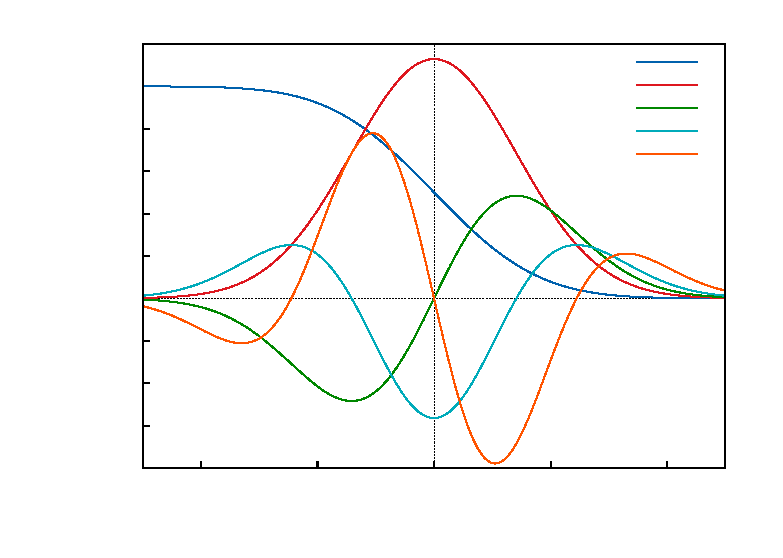
\includegraphics{./figures/gmf_tail}}%
    \gplfronttext
  \end{picture}%
\endgroup
}
%  \caption{First 4 GMF for $\std^2=2$ and $\HS=\HST=\uinf$}
%\end{figure}
\item Derivatives:
\begin{equation}
  \forall j, \ \ \frac{\text{d}\GMFa_j}{\text{d}\lset}(\HST)=(-1)^j\frac{\text{d}^{j+1}\TP(\lset)}{\text{d}\lset^{j+1}}=-\GMFa_{j+1}(\HST)
\end{equation}
\end{itemize}

\subsubsection{Application to one-dimensional cumulative hitting set: $k=1$ and $\HS=\minfu$}
Cumulative probability $\CDP$:
\begin{equation}
  \GaussMeas^1(\minfu) = \Proba\{\GRV\le\lset\}=\frac{1}{\std\sqrt{2\pi}} \int_{-\infty}^\lset e^{-(x-\mean)^2/2\std^2} dx=\CDP(\lset)
\end{equation}
Error function $\erf$:
\begin{equation}
  \GaussMeas^1(\minfu)=\CDP(\lset)=\frac{1}{2}\left(1+\erf\left(\frac{\lset-\mean}{\std\sqrt{2}}\right)\right)
\end{equation}
Tube expension:
\begin{equation}
  \GaussMeas^1(\tube(\minfu,\ray))=\GaussMeas^1((-\infty\ \lset+\ray])=\CDP(\lset+\ray)=\sum_{j=0}^{\infty} \frac{\ray^j}{j!} \frac{\text{d}^j \CDP(\lset)}{\text{d} \lset^j}
\end{equation}
Identification:
\begin{itemize}
\item Notations:
  \begin{subequations}
    \begin{flalign}
      & \text{Tail hitting set:} \ \ \HSC=\minfu & \\
      & \text{Variable substitution:} \ \ \clset \leftarrow \frac{\lset-\mean}{\std} &
    \end{flalign}
  \end{subequations}
\item For $j=0$:
\begin{equation}
  \GMFa_0(\HSC)=\CDP(\lset)
\end{equation}
\item For $j>0$:
\begin{equation}
  \GMFa_j(\HSC)=\frac{\text{d}^j\CDP(\lset)}{\text{d}\lset^j}=(-1)^{j+1}\frac{e^{-(\lset-\mean)^2/2\std^2}}{\std^j\sqrt{2\pi}}\Hermite_{j-1}((\lset-\mean)/\std)
\end{equation}
\item First values:
\begin{equation}
  \left|
  \begin{array}{l}
    \GMFa_0(\HSC) = \frac{1}{2}\left(1-\erf\left(\frac{\clset}{\sqrt{2}}\right)\right) \\ \\
    \GMFa_1(\HSC) = \frac{1}{\std  \sqrt{2\pi}}\ e^{-\clset^2/2} \\ \\
    \GMFa_2(\HSC) = \frac{-1}{\std^2\sqrt{2\pi}}\ \clset \ e^{-\clset^2/2} \\ \\
    \GMFa_3(\HSC) = \frac{1}{\std^3\sqrt{2\pi}}\ \left(\clset^2-1\right) \ e^{-\clset^2/2} \\ \\
    \GMFa_4(\HSC) = \frac{-1}{\std^4\sqrt{2\pi}}\ \left(\clset^3-3\clset\right) \ e^{-\clset^2/2} \\ \\
    \dots
  \end{array}
  \right.
\end{equation}
\begin{figure}[!h]
  \centering
  \hspace*{\fill}
  \subfigure[$\HS=\HSC=\uinf$]{\scalebox{0.5}{% GNUPLOT: LaTeX picture with Postscript
\begingroup
  \makeatletter
  \providecommand\color[2][]{%
    \GenericError{(gnuplot) \space\space\space\@spaces}{%
      Package color not loaded in conjunction with
      terminal option `colourtext'%
    }{See the gnuplot documentation for explanation.%
    }{Either use 'blacktext' in gnuplot or load the package
      color.sty in LaTeX.}%
    \renewcommand\color[2][]{}%
  }%
  \providecommand\includegraphics[2][]{%
    \GenericError{(gnuplot) \space\space\space\@spaces}{%
      Package graphicx or graphics not loaded%
    }{See the gnuplot documentation for explanation.%
    }{The gnuplot epslatex terminal needs graphicx.sty or graphics.sty.}%
    \renewcommand\includegraphics[2][]{}%
  }%
  \providecommand\rotatebox[2]{#2}%
  \@ifundefined{ifGPcolor}{%
    \newif\ifGPcolor
    \GPcolorfalse
  }{}%
  \@ifundefined{ifGPblacktext}{%
    \newif\ifGPblacktext
    \GPblacktexttrue
  }{}%
  % define a \g@addto@macro without @ in the name:
  \let\gplgaddtomacro\g@addto@macro
  % define empty templates for all commands taking text:
  \gdef\gplbacktext{}%
  \gdef\gplfronttext{}%
  \makeatother
  \ifGPblacktext
    % no textcolor at all
    \def\colorrgb#1{}%
    \def\colorgray#1{}%
  \else
    % gray or color?
    \ifGPcolor
      \def\colorrgb#1{\color[rgb]{#1}}%
      \def\colorgray#1{\color[gray]{#1}}%
      \expandafter\def\csname LTw\endcsname{\color{white}}%
      \expandafter\def\csname LTb\endcsname{\color{black}}%
      \expandafter\def\csname LTa\endcsname{\color{black}}%
      \expandafter\def\csname LT0\endcsname{\color[rgb]{1,0,0}}%
      \expandafter\def\csname LT1\endcsname{\color[rgb]{0,1,0}}%
      \expandafter\def\csname LT2\endcsname{\color[rgb]{0,0,1}}%
      \expandafter\def\csname LT3\endcsname{\color[rgb]{1,0,1}}%
      \expandafter\def\csname LT4\endcsname{\color[rgb]{0,1,1}}%
      \expandafter\def\csname LT5\endcsname{\color[rgb]{1,1,0}}%
      \expandafter\def\csname LT6\endcsname{\color[rgb]{0,0,0}}%
      \expandafter\def\csname LT7\endcsname{\color[rgb]{1,0.3,0}}%
      \expandafter\def\csname LT8\endcsname{\color[rgb]{0.5,0.5,0.5}}%
    \else
      % gray
      \def\colorrgb#1{\color{black}}%
      \def\colorgray#1{\color[gray]{#1}}%
      \expandafter\def\csname LTw\endcsname{\color{white}}%
      \expandafter\def\csname LTb\endcsname{\color{black}}%
      \expandafter\def\csname LTa\endcsname{\color{black}}%
      \expandafter\def\csname LT0\endcsname{\color{black}}%
      \expandafter\def\csname LT1\endcsname{\color{black}}%
      \expandafter\def\csname LT2\endcsname{\color{black}}%
      \expandafter\def\csname LT3\endcsname{\color{black}}%
      \expandafter\def\csname LT4\endcsname{\color{black}}%
      \expandafter\def\csname LT5\endcsname{\color{black}}%
      \expandafter\def\csname LT6\endcsname{\color{black}}%
      \expandafter\def\csname LT7\endcsname{\color{black}}%
      \expandafter\def\csname LT8\endcsname{\color{black}}%
    \fi
  \fi
  \setlength{\unitlength}{0.0500bp}%
  \begin{picture}(7200.00,5040.00)%
    \gplgaddtomacro\gplbacktext{%
      \csname LTb\endcsname%
      \put(1078,704){\makebox(0,0)[r]{\strut{}-0.2}}%
      \put(1078,1111){\makebox(0,0)[r]{\strut{}-0.15}}%
      \put(1078,1518){\makebox(0,0)[r]{\strut{}-0.1}}%
      \put(1078,1925){\makebox(0,0)[r]{\strut{}-0.05}}%
      \put(1078,2332){\makebox(0,0)[r]{\strut{} 0}}%
      \put(1078,2740){\makebox(0,0)[r]{\strut{} 0.05}}%
      \put(1078,3147){\makebox(0,0)[r]{\strut{} 0.1}}%
      \put(1078,3554){\makebox(0,0)[r]{\strut{} 0.15}}%
      \put(1078,3961){\makebox(0,0)[r]{\strut{} 0.2}}%
      \put(1078,4368){\makebox(0,0)[r]{\strut{} 0.25}}%
      \put(1078,4775){\makebox(0,0)[r]{\strut{} 0.3}}%
      \put(1769,484){\makebox(0,0){\strut{}-4}}%
      \put(2888,484){\makebox(0,0){\strut{}-2}}%
      \put(4007,484){\makebox(0,0){\strut{} 0}}%
      \put(5125,484){\makebox(0,0){\strut{} 2}}%
      \put(6244,484){\makebox(0,0){\strut{} 4}}%
      \csname LTb\endcsname%
      \put(176,2739){\rotatebox{90}{\makebox(0,0){\strut{}$\GMFa_j(\HST)$}}}%
      \put(4006,154){\makebox(0,0){\strut{}$\lset$}}%
    }%
    \gplgaddtomacro\gplfronttext{%
      \csname LTb\endcsname%
      \put(5816,4602){\makebox(0,0)[r]{\strut{}$j=0$ ($\bullet/4$)}}%
      \csname LTb\endcsname%
      \put(5816,4382){\makebox(0,0)[r]{\strut{}$j=1$}}%
      \csname LTb\endcsname%
      \put(5816,4162){\makebox(0,0)[r]{\strut{}$j=2$}}%
      \csname LTb\endcsname%
      \put(5816,3942){\makebox(0,0)[r]{\strut{}$j=3$}}%
      \csname LTb\endcsname%
      \put(5816,3722){\makebox(0,0)[r]{\strut{}$j=4$}}%
    }%
    \gplbacktext
    \put(0,0){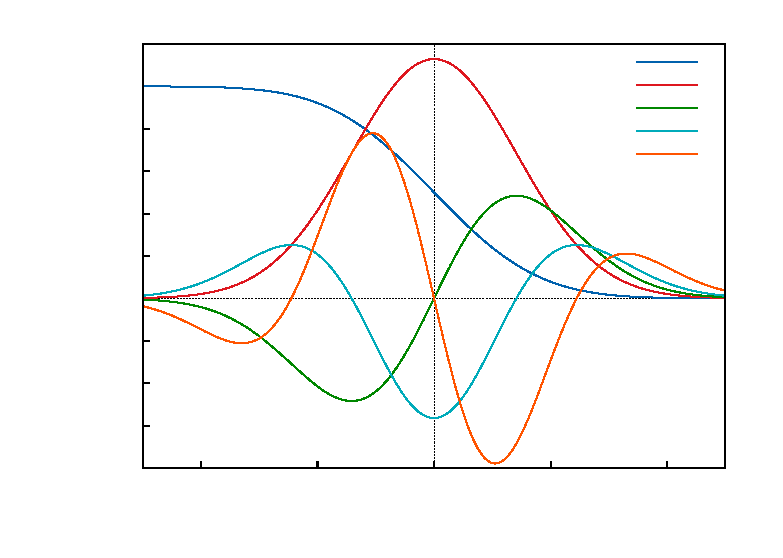
\includegraphics{./figures/gmf_tail}}%
    \gplfronttext
  \end{picture}%
\endgroup
}}\hfill
  \subfigure[$\HS=\HSC=\minfu$]{\scalebox{0.5}{% GNUPLOT: LaTeX picture with Postscript
\begingroup
  \makeatletter
  \providecommand\color[2][]{%
    \GenericError{(gnuplot) \space\space\space\@spaces}{%
      Package color not loaded in conjunction with
      terminal option `colourtext'%
    }{See the gnuplot documentation for explanation.%
    }{Either use 'blacktext' in gnuplot or load the package
      color.sty in LaTeX.}%
    \renewcommand\color[2][]{}%
  }%
  \providecommand\includegraphics[2][]{%
    \GenericError{(gnuplot) \space\space\space\@spaces}{%
      Package graphicx or graphics not loaded%
    }{See the gnuplot documentation for explanation.%
    }{The gnuplot epslatex terminal needs graphicx.sty or graphics.sty.}%
    \renewcommand\includegraphics[2][]{}%
  }%
  \providecommand\rotatebox[2]{#2}%
  \@ifundefined{ifGPcolor}{%
    \newif\ifGPcolor
    \GPcolorfalse
  }{}%
  \@ifundefined{ifGPblacktext}{%
    \newif\ifGPblacktext
    \GPblacktexttrue
  }{}%
  % define a \g@addto@macro without @ in the name:
  \let\gplgaddtomacro\g@addto@macro
  % define empty templates for all commands taking text:
  \gdef\gplbacktext{}%
  \gdef\gplfronttext{}%
  \makeatother
  \ifGPblacktext
    % no textcolor at all
    \def\colorrgb#1{}%
    \def\colorgray#1{}%
  \else
    % gray or color?
    \ifGPcolor
      \def\colorrgb#1{\color[rgb]{#1}}%
      \def\colorgray#1{\color[gray]{#1}}%
      \expandafter\def\csname LTw\endcsname{\color{white}}%
      \expandafter\def\csname LTb\endcsname{\color{black}}%
      \expandafter\def\csname LTa\endcsname{\color{black}}%
      \expandafter\def\csname LT0\endcsname{\color[rgb]{1,0,0}}%
      \expandafter\def\csname LT1\endcsname{\color[rgb]{0,1,0}}%
      \expandafter\def\csname LT2\endcsname{\color[rgb]{0,0,1}}%
      \expandafter\def\csname LT3\endcsname{\color[rgb]{1,0,1}}%
      \expandafter\def\csname LT4\endcsname{\color[rgb]{0,1,1}}%
      \expandafter\def\csname LT5\endcsname{\color[rgb]{1,1,0}}%
      \expandafter\def\csname LT6\endcsname{\color[rgb]{0,0,0}}%
      \expandafter\def\csname LT7\endcsname{\color[rgb]{1,0.3,0}}%
      \expandafter\def\csname LT8\endcsname{\color[rgb]{0.5,0.5,0.5}}%
    \else
      % gray
      \def\colorrgb#1{\color{black}}%
      \def\colorgray#1{\color[gray]{#1}}%
      \expandafter\def\csname LTw\endcsname{\color{white}}%
      \expandafter\def\csname LTb\endcsname{\color{black}}%
      \expandafter\def\csname LTa\endcsname{\color{black}}%
      \expandafter\def\csname LT0\endcsname{\color{black}}%
      \expandafter\def\csname LT1\endcsname{\color{black}}%
      \expandafter\def\csname LT2\endcsname{\color{black}}%
      \expandafter\def\csname LT3\endcsname{\color{black}}%
      \expandafter\def\csname LT4\endcsname{\color{black}}%
      \expandafter\def\csname LT5\endcsname{\color{black}}%
      \expandafter\def\csname LT6\endcsname{\color{black}}%
      \expandafter\def\csname LT7\endcsname{\color{black}}%
      \expandafter\def\csname LT8\endcsname{\color{black}}%
    \fi
  \fi
  \setlength{\unitlength}{0.0500bp}%
  \begin{picture}(7200.00,5040.00)%
    \gplgaddtomacro\gplbacktext{%
      \csname LTb\endcsname%
      \put(1078,704){\makebox(0,0)[r]{\strut{}-0.2}}%
      \put(1078,1111){\makebox(0,0)[r]{\strut{}-0.15}}%
      \put(1078,1518){\makebox(0,0)[r]{\strut{}-0.1}}%
      \put(1078,1925){\makebox(0,0)[r]{\strut{}-0.05}}%
      \put(1078,2332){\makebox(0,0)[r]{\strut{} 0}}%
      \put(1078,2740){\makebox(0,0)[r]{\strut{} 0.05}}%
      \put(1078,3147){\makebox(0,0)[r]{\strut{} 0.1}}%
      \put(1078,3554){\makebox(0,0)[r]{\strut{} 0.15}}%
      \put(1078,3961){\makebox(0,0)[r]{\strut{} 0.2}}%
      \put(1078,4368){\makebox(0,0)[r]{\strut{} 0.25}}%
      \put(1078,4775){\makebox(0,0)[r]{\strut{} 0.3}}%
      \put(1769,484){\makebox(0,0){\strut{}-4}}%
      \put(2888,484){\makebox(0,0){\strut{}-2}}%
      \put(4007,484){\makebox(0,0){\strut{} 0}}%
      \put(5125,484){\makebox(0,0){\strut{} 2}}%
      \put(6244,484){\makebox(0,0){\strut{} 4}}%
      \csname LTb\endcsname%
      \put(176,2739){\rotatebox{90}{\makebox(0,0){\strut{}$\GMFa_j(\HSC)$}}}%
      \put(4006,154){\makebox(0,0){\strut{}$\lset$}}%
    }%
    \gplgaddtomacro\gplfronttext{%
      \csname LTb\endcsname%
      \put(2530,4602){\makebox(0,0)[r]{\strut{}$j=0$ ($\bullet/4$)}}%
      \csname LTb\endcsname%
      \put(2530,4382){\makebox(0,0)[r]{\strut{}$j=1$}}%
      \csname LTb\endcsname%
      \put(2530,4162){\makebox(0,0)[r]{\strut{}$j=2$}}%
      \csname LTb\endcsname%
      \put(2530,3942){\makebox(0,0)[r]{\strut{}$j=3$}}%
      \csname LTb\endcsname%
      \put(2530,3722){\makebox(0,0)[r]{\strut{}$j=4$}}%
    }%
    \gplbacktext
    \put(0,0){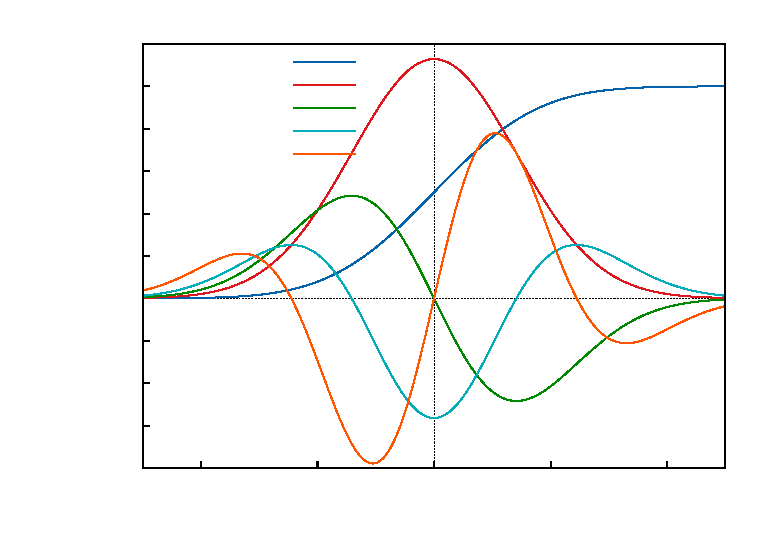
\includegraphics{./figures/gmf_cumulative}}%
    \gplfronttext
  \end{picture}%
\endgroup
}}\hspace*{\fill}
  \caption{First 4 GMF for $\std^2=2$}
\end{figure}
\item Derivatives:
\begin{equation}
  \forall j, \ \ \frac{\text{d}\GMFa_j}{\text{d}\lset}(\HSC)=\frac{\text{d}^{j+1}\CDP(\lset)}{\text{d}\lset^{j+1}}=\GMFa_{j+1}(\HSC)
\end{equation}
\end{itemize}

\subsection{GMFs for Gaussian related Random Fields}
\begin{equation}
  \GRRF : \Univ\times\RN \overset{\vGRF}{\rightarrow} \Rk \overset{\rfunc}{\rightarrow} \RR
\end{equation}
\begin{equation}
    \Proba\left\{\GRRF\in\HS\right\} = \Proba\left\{\rfunc(\GRF)\in\HS\right\} = \Proba\left\{\GRF\in\irfunc(\HS)\right\} = \GaussMeas^k(\irfunc(\HS))
\end{equation}

\subsubsection{Log-normal distribution}
\begin{equation}
  k=1 \ \ \text{,} \ \ \rfunc=\exp \ \ \text{and} \ \ \irfunc=\ln
\end{equation}
\begin{equation}
  \left|
  \begin{array}{lcl}
    \mean & = &\ln(\meanln) - \frac{1}{2}\ln(1+\stdln^2/\meanln^2) \\
    \std^2 & = & \ln(1+\stdln^2/\meanln^2)
  \end{array}
  \right.
\end{equation}

\begin{itemize}
\item Notations:
  \begin{subequations}
    \begin{flalign}
      & \text{Log tail hitting set:} \ \ \lnHST=\lnuinf & \\
      & \text{Log cumulative hitting set:} \ \ \lnHSC = \minflnu & \\
      & \text{Variable substitution:} \ \ \lnclset \leftarrow \frac{\ln(\lset)-\mean}{\std} &
    \end{flalign}
  \end{subequations}
\item For $\HS=\HST=\uinf \ \ \rightarrow \ \ \irfunc(\HS) = \lnHST = \lnuinf$
\begin{equation}
  \left|
  \begin{array}{l}
    \GMFa_0(\lnHST) = \frac{1}{2}\left(1-\erf\left(\frac{\lnclset}{\sqrt{2}}\right)\right) \\ \\
    \GMFa_1(\lnHST) = \frac{1}{\std  \sqrt{2\pi}}\ e^{-\lnclset^2/2} \\ \\
    \GMFa_2(\lnHST) = \frac{1}{\std^2\sqrt{2\pi}}\ \lnclset \ e^{-\lnclset^2/2} \\ \\
    \GMFa_3(\lnHST) = \frac{1}{\std^3\sqrt{2\pi}}\ \left(\lnclset^2-1\right) \ e^{-\lnclset^2/2} \\ \\
    \GMFa_4(\lnHST) = \frac{1}{\std^4\sqrt{2\pi}}\ \left(\lnclset^3-3\lnclset\right) \ e^{-\lnclset^2/2} \\ \\
    \dots
  \end{array}
  \right.
\end{equation}
Derivatives:
\begin{equation}
  \left|
  \begin{array}{l}
    \text{Help:} \ \ \left(e^{-(\ln(x)-\mean)^2/2\std^2}\right)' = -\frac{1}{\std^2} \frac{\ln(x)-\mean}{x}\ e^{-(\ln(x)-\mean)^2/2\std^2} \\ \\
    \frac{\text{d} \GMFa_0(\lnHST)}{\text{d}\lset} = \frac{-1}{\std\sqrt{2\pi}} \frac{1}{\lset}\ e^{-(\ln(\lset)-\mean)^2/2\std^2} \\ \\
    \frac{\text{d} \GMFa_1(\lnHST)}{\text{d}\lset} = \frac{-1}{\std^2\sqrt{2\pi}} \frac{1}{\lset}\frac{\ln(\lset)-\mean}{\std}\ e^{-(\ln(\lset)-\mean)^2/2\std^2} \\ \\
    \frac{\text{d} \GMFa_2(\lnHST)}{\text{d}\lset} = \frac{-1}{\std^3\sqrt{2\pi}} \frac{1}{\lset}\left[ \frac{(\ln(\lset)-\mean)^2}{\std^2} - 1 \right]\ e^{-(\ln(\lset)-\mean)^2/2\std^2} \\ \\
    \frac{\text{d} \GMFa_3(\lnHST)}{\text{d}\lset} = \frac{-1}{\std^4\sqrt{2\pi}} \frac{1}{\lset}\left[ \frac{(\ln(\lset)-\mean)^3}{\std^3} - 3\frac{(\ln(\lset)-\mean)}{\std} \right]\ e^{-(\ln(\lset)-\mean)^2/2\std^2} \\ \\
    \dots \\ \\
    \text{Guess would be:} \ \ \forall j\ge0, \\
    \frac{\text{d} \GMFa_j(\lnHST)}{\text{d}\lset} = \frac{-1}{\std^{j+1}\sqrt{2\pi}}\frac{1}{\lset}\Hermite_{j}(\lnclset)\ e^{-\lnclset^2/2}
  \end{array}
  \right.
\end{equation}

\item For $\HS=\zu \ \ \rightarrow \ \ \irfunc(\HS) = \lnHSC = \minflnu$
\begin{equation}
  \left|
  \begin{array}{l}
    \GMFa_0(\lnHSC) = \frac{1}{2}\left(1+\erf\left(\frac{\lnclset}{\sqrt{2}}\right)\right) \\ \\
    \GMFa_1(\lnHSC) = \frac{1}{\std  \sqrt{2\pi}}\ e^{-\lnclset^2/2} \\ \\
    \GMFa_2(\lnHSC) = \frac{-1}{\std^2\sqrt{2\pi}}\ \lnclset \ e^{-\lnclset^2/2} \\ \\
    \GMFa_3(\lnHSC) = \frac{1}{\std^3\sqrt{2\pi}}\ \left(\lnclset^2-1\right) \ e^{-\lnclset^2/2} \\ \\
    \GMFa_4(\lnHSC) = \frac{-1}{\std^4\sqrt{2\pi}}\ \left(\lnclset^3-3\lnclset\right) \ e^{-\lnclset^2/2} \\ \\
    \dots
  \end{array}
  \right.
\end{equation}
Derivatives:
\begin{equation}
  \left|
  \begin{array}{l}
    \text{Guess would be:} \ \ \forall j\ge0, \\
    \frac{\text{d} \GMFa_j(\lnHSC)}{\text{d}\lset} = \frac{(-1)^{j}}{\std^{j+1}\sqrt{2\pi}}\frac{1}{\lset}\Hermite_{j}(\lnclset)\ e^{-\lnclset^2/2}
  \end{array}
  \right.
\end{equation}

\end{itemize}

\newpage
\section{Expectation Formula}
\subsection{Gaussian distribution}
\subsubsection{General case}
\begin{equation}
  \Expec\left\{\ \LKC_j(\ES) \ \right\} = \sum_{i=0}^{N-j} \left[ \begin{array}{c}i+j\\i\end{array}\right]\left(\frac{\SpecMom}{2\pi}\right)^{i/2}\LKC_{i+j}(\MRF)\GMFk_i(\irfunc(\HS))
\end{equation}
Notations:
  \begin{subequations}
    \begin{flalign}
      & \text{LKC of $\MRF$:} \ \ \LKC_j(\MRF) = \LKC_j^\MRF & \\
      & \text{LKC of $\ES$:} \ \ \LKC_j(\ES) = \LKC_j^\ES & \\
      & \text{GMF of $\irfunc(\HS)$:} \ \  \GMFk_j(\irfunc(\HS)) = \GMFk_j
    \end{flalign}
  \end{subequations}
\subsubsection{One dimension}
\begin{subequations}
\begin{align}
  &\Expec\left\{\LKC_0^\ES\right\} = \left(\frac{\SpecMom}{2\pi}\right)^{1/2}\LKC_1^\MRF\GMFk_1 + \LKC_0^\MRF\GMFk_0\\
  &\Expec\left\{\LKC_1^\ES\right\} = \LKC_1^\MRF\GMFk_0
\end{align}
\end{subequations}


\begin{figure}[!h]
  \centering
  \hspace*{\fill}
  \subfigure[Euler Characteristic]{\scalebox{0.5}{% GNUPLOT: LaTeX picture with Postscript
\begingroup
  \makeatletter
  \providecommand\color[2][]{%
    \GenericError{(gnuplot) \space\space\space\@spaces}{%
      Package color not loaded in conjunction with
      terminal option `colourtext'%
    }{See the gnuplot documentation for explanation.%
    }{Either use 'blacktext' in gnuplot or load the package
      color.sty in LaTeX.}%
    \renewcommand\color[2][]{}%
  }%
  \providecommand\includegraphics[2][]{%
    \GenericError{(gnuplot) \space\space\space\@spaces}{%
      Package graphicx or graphics not loaded%
    }{See the gnuplot documentation for explanation.%
    }{The gnuplot epslatex terminal needs graphicx.sty or graphics.sty.}%
    \renewcommand\includegraphics[2][]{}%
  }%
  \providecommand\rotatebox[2]{#2}%
  \@ifundefined{ifGPcolor}{%
    \newif\ifGPcolor
    \GPcolorfalse
  }{}%
  \@ifundefined{ifGPblacktext}{%
    \newif\ifGPblacktext
    \GPblacktexttrue
  }{}%
  % define a \g@addto@macro without @ in the name:
  \let\gplgaddtomacro\g@addto@macro
  % define empty templates for all commands taking text:
  \gdef\gplbacktext{}%
  \gdef\gplfronttext{}%
  \makeatother
  \ifGPblacktext
    % no textcolor at all
    \def\colorrgb#1{}%
    \def\colorgray#1{}%
  \else
    % gray or color?
    \ifGPcolor
      \def\colorrgb#1{\color[rgb]{#1}}%
      \def\colorgray#1{\color[gray]{#1}}%
      \expandafter\def\csname LTw\endcsname{\color{white}}%
      \expandafter\def\csname LTb\endcsname{\color{black}}%
      \expandafter\def\csname LTa\endcsname{\color{black}}%
      \expandafter\def\csname LT0\endcsname{\color[rgb]{1,0,0}}%
      \expandafter\def\csname LT1\endcsname{\color[rgb]{0,1,0}}%
      \expandafter\def\csname LT2\endcsname{\color[rgb]{0,0,1}}%
      \expandafter\def\csname LT3\endcsname{\color[rgb]{1,0,1}}%
      \expandafter\def\csname LT4\endcsname{\color[rgb]{0,1,1}}%
      \expandafter\def\csname LT5\endcsname{\color[rgb]{1,1,0}}%
      \expandafter\def\csname LT6\endcsname{\color[rgb]{0,0,0}}%
      \expandafter\def\csname LT7\endcsname{\color[rgb]{1,0.3,0}}%
      \expandafter\def\csname LT8\endcsname{\color[rgb]{0.5,0.5,0.5}}%
    \else
      % gray
      \def\colorrgb#1{\color{black}}%
      \def\colorgray#1{\color[gray]{#1}}%
      \expandafter\def\csname LTw\endcsname{\color{white}}%
      \expandafter\def\csname LTb\endcsname{\color{black}}%
      \expandafter\def\csname LTa\endcsname{\color{black}}%
      \expandafter\def\csname LT0\endcsname{\color{black}}%
      \expandafter\def\csname LT1\endcsname{\color{black}}%
      \expandafter\def\csname LT2\endcsname{\color{black}}%
      \expandafter\def\csname LT3\endcsname{\color{black}}%
      \expandafter\def\csname LT4\endcsname{\color{black}}%
      \expandafter\def\csname LT5\endcsname{\color{black}}%
      \expandafter\def\csname LT6\endcsname{\color{black}}%
      \expandafter\def\csname LT7\endcsname{\color{black}}%
      \expandafter\def\csname LT8\endcsname{\color{black}}%
    \fi
  \fi
  \setlength{\unitlength}{0.0500bp}%
  \begin{picture}(7200.00,5040.00)%
    \gplgaddtomacro\gplbacktext{%
      \csname LTb\endcsname%
      \put(946,704){\makebox(0,0)[r]{\strut{} 0}}%
      \put(946,1213){\makebox(0,0)[r]{\strut{} 0.2}}%
      \put(946,1722){\makebox(0,0)[r]{\strut{} 0.4}}%
      \put(946,2231){\makebox(0,0)[r]{\strut{} 0.6}}%
      \put(946,2740){\makebox(0,0)[r]{\strut{} 0.8}}%
      \put(946,3248){\makebox(0,0)[r]{\strut{} 1}}%
      \put(946,3757){\makebox(0,0)[r]{\strut{} 1.2}}%
      \put(946,4266){\makebox(0,0)[r]{\strut{} 1.4}}%
      \put(946,4775){\makebox(0,0)[r]{\strut{} 1.6}}%
      \put(1651,484){\makebox(0,0){\strut{}-4}}%
      \put(2796,484){\makebox(0,0){\strut{}-2}}%
      \put(3941,484){\makebox(0,0){\strut{} 0}}%
      \put(5086,484){\makebox(0,0){\strut{} 2}}%
      \put(6231,484){\makebox(0,0){\strut{} 4}}%
      \csname LTb\endcsname%
      \put(176,2739){\rotatebox{90}{\makebox(0,0){\strut{}Euleru characteristic}}}%
      \put(3940,154){\makebox(0,0){\strut{}$\lset$}}%
    }%
    \gplgaddtomacro\gplfronttext{%
      \csname LTb\endcsname%
      \put(5816,4602){\makebox(0,0)[r]{\strut{}$\Lc=25$}}%
      \csname LTb\endcsname%
      \put(5816,4382){\makebox(0,0)[r]{\strut{}$\Lc=50$}}%
      \csname LTb\endcsname%
      \put(5816,4162){\makebox(0,0)[r]{\strut{}$\Lc=100$}}%
      \csname LTb\endcsname%
      \put(5816,3942){\makebox(0,0)[r]{\strut{}$\Lc=500$}}%
      \csname LTb\endcsname%
      \put(5816,3722){\makebox(0,0)[r]{\strut{}$\Lc=1000$}}%
    }%
    \gplbacktext
    \put(0,0){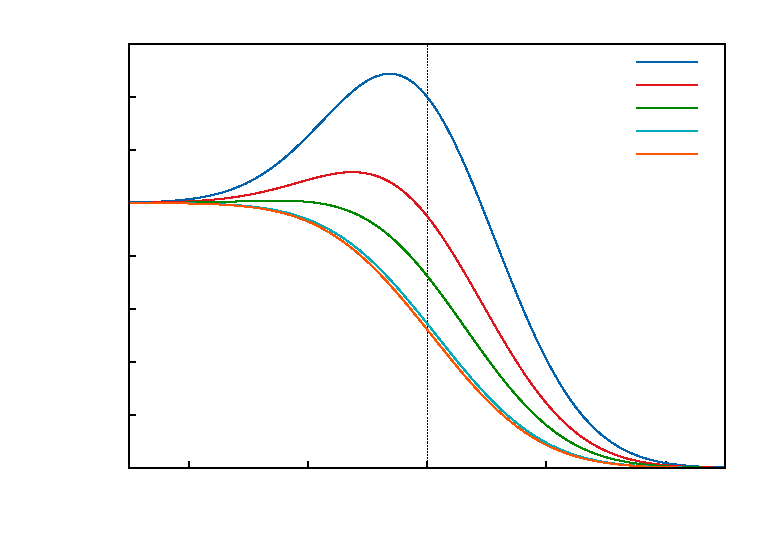
\includegraphics{./figures/elkc_1D_LKC0}}%
    \gplfronttext
  \end{picture}%
\endgroup
}}\hfill
  \subfigure[Length]{\scalebox{0.5}{% GNUPLOT: LaTeX picture with Postscript
\begingroup
  \makeatletter
  \providecommand\color[2][]{%
    \GenericError{(gnuplot) \space\space\space\@spaces}{%
      Package color not loaded in conjunction with
      terminal option `colourtext'%
    }{See the gnuplot documentation for explanation.%
    }{Either use 'blacktext' in gnuplot or load the package
      color.sty in LaTeX.}%
    \renewcommand\color[2][]{}%
  }%
  \providecommand\includegraphics[2][]{%
    \GenericError{(gnuplot) \space\space\space\@spaces}{%
      Package graphicx or graphics not loaded%
    }{See the gnuplot documentation for explanation.%
    }{The gnuplot epslatex terminal needs graphicx.sty or graphics.sty.}%
    \renewcommand\includegraphics[2][]{}%
  }%
  \providecommand\rotatebox[2]{#2}%
  \@ifundefined{ifGPcolor}{%
    \newif\ifGPcolor
    \GPcolorfalse
  }{}%
  \@ifundefined{ifGPblacktext}{%
    \newif\ifGPblacktext
    \GPblacktexttrue
  }{}%
  % define a \g@addto@macro without @ in the name:
  \let\gplgaddtomacro\g@addto@macro
  % define empty templates for all commands taking text:
  \gdef\gplbacktext{}%
  \gdef\gplfronttext{}%
  \makeatother
  \ifGPblacktext
    % no textcolor at all
    \def\colorrgb#1{}%
    \def\colorgray#1{}%
  \else
    % gray or color?
    \ifGPcolor
      \def\colorrgb#1{\color[rgb]{#1}}%
      \def\colorgray#1{\color[gray]{#1}}%
      \expandafter\def\csname LTw\endcsname{\color{white}}%
      \expandafter\def\csname LTb\endcsname{\color{black}}%
      \expandafter\def\csname LTa\endcsname{\color{black}}%
      \expandafter\def\csname LT0\endcsname{\color[rgb]{1,0,0}}%
      \expandafter\def\csname LT1\endcsname{\color[rgb]{0,1,0}}%
      \expandafter\def\csname LT2\endcsname{\color[rgb]{0,0,1}}%
      \expandafter\def\csname LT3\endcsname{\color[rgb]{1,0,1}}%
      \expandafter\def\csname LT4\endcsname{\color[rgb]{0,1,1}}%
      \expandafter\def\csname LT5\endcsname{\color[rgb]{1,1,0}}%
      \expandafter\def\csname LT6\endcsname{\color[rgb]{0,0,0}}%
      \expandafter\def\csname LT7\endcsname{\color[rgb]{1,0.3,0}}%
      \expandafter\def\csname LT8\endcsname{\color[rgb]{0.5,0.5,0.5}}%
    \else
      % gray
      \def\colorrgb#1{\color{black}}%
      \def\colorgray#1{\color[gray]{#1}}%
      \expandafter\def\csname LTw\endcsname{\color{white}}%
      \expandafter\def\csname LTb\endcsname{\color{black}}%
      \expandafter\def\csname LTa\endcsname{\color{black}}%
      \expandafter\def\csname LT0\endcsname{\color{black}}%
      \expandafter\def\csname LT1\endcsname{\color{black}}%
      \expandafter\def\csname LT2\endcsname{\color{black}}%
      \expandafter\def\csname LT3\endcsname{\color{black}}%
      \expandafter\def\csname LT4\endcsname{\color{black}}%
      \expandafter\def\csname LT5\endcsname{\color{black}}%
      \expandafter\def\csname LT6\endcsname{\color{black}}%
      \expandafter\def\csname LT7\endcsname{\color{black}}%
      \expandafter\def\csname LT8\endcsname{\color{black}}%
    \fi
  \fi
  \setlength{\unitlength}{0.0500bp}%
  \begin{picture}(7200.00,5040.00)%
    \gplgaddtomacro\gplbacktext{%
      \csname LTb\endcsname%
      \put(946,704){\makebox(0,0)[r]{\strut{} 0}}%
      \put(946,1111){\makebox(0,0)[r]{\strut{} 10}}%
      \put(946,1518){\makebox(0,0)[r]{\strut{} 20}}%
      \put(946,1925){\makebox(0,0)[r]{\strut{} 30}}%
      \put(946,2332){\makebox(0,0)[r]{\strut{} 40}}%
      \put(946,2740){\makebox(0,0)[r]{\strut{} 50}}%
      \put(946,3147){\makebox(0,0)[r]{\strut{} 60}}%
      \put(946,3554){\makebox(0,0)[r]{\strut{} 70}}%
      \put(946,3961){\makebox(0,0)[r]{\strut{} 80}}%
      \put(946,4368){\makebox(0,0)[r]{\strut{} 90}}%
      \put(946,4775){\makebox(0,0)[r]{\strut{} 100}}%
      \put(1651,484){\makebox(0,0){\strut{}-4}}%
      \put(2796,484){\makebox(0,0){\strut{}-2}}%
      \put(3941,484){\makebox(0,0){\strut{} 0}}%
      \put(5086,484){\makebox(0,0){\strut{} 2}}%
      \put(6231,484){\makebox(0,0){\strut{} 4}}%
      \csname LTb\endcsname%
      \put(176,2739){\rotatebox{90}{\makebox(0,0){\strut{}Length}}}%
      \put(3940,154){\makebox(0,0){\strut{}$\lset$}}%
    }%
    \gplgaddtomacro\gplfronttext{%
    }%
    \gplbacktext
    \put(0,0){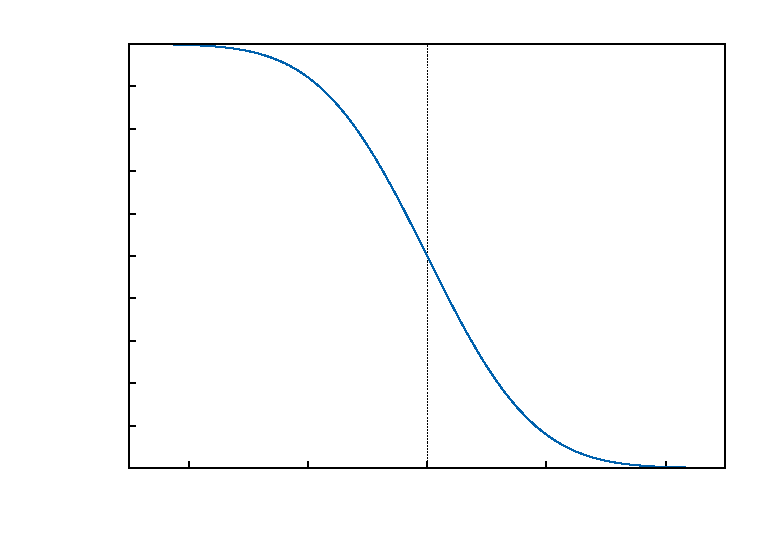
\includegraphics{./figures/elkc_1D_LKC1}}%
    \gplfronttext
  \end{picture}%
\endgroup
}}\hspace*{\fill}
  \caption{Expectation of LKC for $\Msize=100$, $\std^2=2$ and $\HS=\uinf$ in 1D.}
\end{figure}

\begin{figure}[!h]
  \centering
  \hspace*{\fill}
  \subfigure{\scalebox{0.5}{% GNUPLOT: LaTeX picture with Postscript
\begingroup
  \makeatletter
  \providecommand\color[2][]{%
    \GenericError{(gnuplot) \space\space\space\@spaces}{%
      Package color not loaded in conjunction with
      terminal option `colourtext'%
    }{See the gnuplot documentation for explanation.%
    }{Either use 'blacktext' in gnuplot or load the package
      color.sty in LaTeX.}%
    \renewcommand\color[2][]{}%
  }%
  \providecommand\includegraphics[2][]{%
    \GenericError{(gnuplot) \space\space\space\@spaces}{%
      Package graphicx or graphics not loaded%
    }{See the gnuplot documentation for explanation.%
    }{The gnuplot epslatex terminal needs graphicx.sty or graphics.sty.}%
    \renewcommand\includegraphics[2][]{}%
  }%
  \providecommand\rotatebox[2]{#2}%
  \@ifundefined{ifGPcolor}{%
    \newif\ifGPcolor
    \GPcolorfalse
  }{}%
  \@ifundefined{ifGPblacktext}{%
    \newif\ifGPblacktext
    \GPblacktexttrue
  }{}%
  % define a \g@addto@macro without @ in the name:
  \let\gplgaddtomacro\g@addto@macro
  % define empty templates for all commands taking text:
  \gdef\gplbacktext{}%
  \gdef\gplfronttext{}%
  \makeatother
  \ifGPblacktext
    % no textcolor at all
    \def\colorrgb#1{}%
    \def\colorgray#1{}%
  \else
    % gray or color?
    \ifGPcolor
      \def\colorrgb#1{\color[rgb]{#1}}%
      \def\colorgray#1{\color[gray]{#1}}%
      \expandafter\def\csname LTw\endcsname{\color{white}}%
      \expandafter\def\csname LTb\endcsname{\color{black}}%
      \expandafter\def\csname LTa\endcsname{\color{black}}%
      \expandafter\def\csname LT0\endcsname{\color[rgb]{1,0,0}}%
      \expandafter\def\csname LT1\endcsname{\color[rgb]{0,1,0}}%
      \expandafter\def\csname LT2\endcsname{\color[rgb]{0,0,1}}%
      \expandafter\def\csname LT3\endcsname{\color[rgb]{1,0,1}}%
      \expandafter\def\csname LT4\endcsname{\color[rgb]{0,1,1}}%
      \expandafter\def\csname LT5\endcsname{\color[rgb]{1,1,0}}%
      \expandafter\def\csname LT6\endcsname{\color[rgb]{0,0,0}}%
      \expandafter\def\csname LT7\endcsname{\color[rgb]{1,0.3,0}}%
      \expandafter\def\csname LT8\endcsname{\color[rgb]{0.5,0.5,0.5}}%
    \else
      % gray
      \def\colorrgb#1{\color{black}}%
      \def\colorgray#1{\color[gray]{#1}}%
      \expandafter\def\csname LTw\endcsname{\color{white}}%
      \expandafter\def\csname LTb\endcsname{\color{black}}%
      \expandafter\def\csname LTa\endcsname{\color{black}}%
      \expandafter\def\csname LT0\endcsname{\color{black}}%
      \expandafter\def\csname LT1\endcsname{\color{black}}%
      \expandafter\def\csname LT2\endcsname{\color{black}}%
      \expandafter\def\csname LT3\endcsname{\color{black}}%
      \expandafter\def\csname LT4\endcsname{\color{black}}%
      \expandafter\def\csname LT5\endcsname{\color{black}}%
      \expandafter\def\csname LT6\endcsname{\color{black}}%
      \expandafter\def\csname LT7\endcsname{\color{black}}%
      \expandafter\def\csname LT8\endcsname{\color{black}}%
    \fi
  \fi
  \setlength{\unitlength}{0.0500bp}%
  \begin{picture}(7200.00,5040.00)%
    \gplgaddtomacro\gplbacktext{%
      \csname LTb\endcsname%
      \put(814,704){\makebox(0,0)[r]{\strut{} 0}}%
      \put(814,1286){\makebox(0,0)[r]{\strut{} 5}}%
      \put(814,1867){\makebox(0,0)[r]{\strut{} 10}}%
      \put(814,2449){\makebox(0,0)[r]{\strut{} 15}}%
      \put(814,3030){\makebox(0,0)[r]{\strut{} 20}}%
      \put(814,3612){\makebox(0,0)[r]{\strut{} 25}}%
      \put(814,4193){\makebox(0,0)[r]{\strut{} 30}}%
      \put(814,4775){\makebox(0,0)[r]{\strut{} 35}}%
      \put(946,484){\makebox(0,0){\strut{} 0.01}}%
      \put(2117,484){\makebox(0,0){\strut{} 0.1}}%
      \put(3289,484){\makebox(0,0){\strut{} 1}}%
      \put(4460,484){\makebox(0,0){\strut{} 10}}%
      \put(5632,484){\makebox(0,0){\strut{} 100}}%
      \put(6803,484){\makebox(0,0){\strut{} 1000}}%
      \csname LTb\endcsname%
      \put(176,2739){\rotatebox{90}{\makebox(0,0){\strut{}Euler characteristic $\EC$}}}%
      \put(3874,154){\makebox(0,0){\strut{}$\lset$}}%
    }%
    \gplgaddtomacro\gplfronttext{%
      \csname LTb\endcsname%
      \put(5816,4602){\makebox(0,0)[r]{\strut{}Experimental}}%
      \csname LTb\endcsname%
      \put(5816,4382){\makebox(0,0)[r]{\strut{}Theoretical}}%
      \csname LTb\endcsname%
      \put(5816,4162){\makebox(0,0)[r]{\strut{}One realization}}%
    }%
    \gplbacktext
    \put(0,0){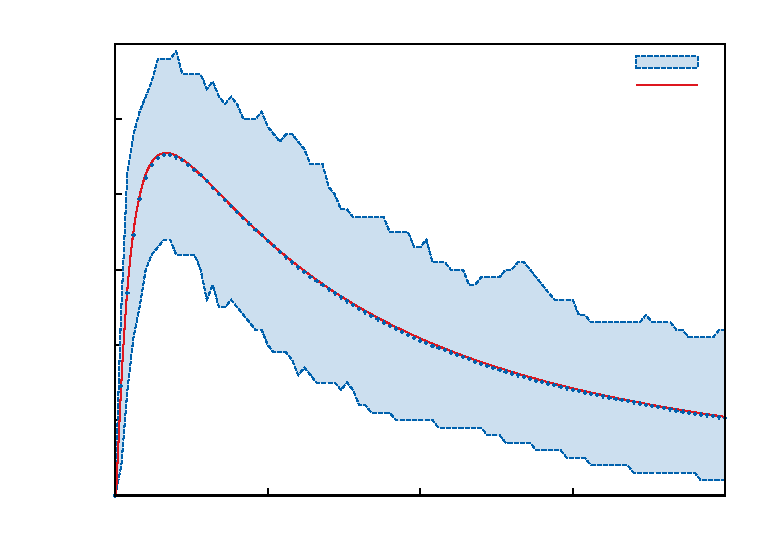
\includegraphics{./figures/elkc_exp_1D_lognormal_0}}%
    \gplfronttext
  \end{picture}%
\endgroup
}}\hfill
  \subfigure{\scalebox{0.5}{% GNUPLOT: LaTeX picture with Postscript
\begingroup
  \makeatletter
  \providecommand\color[2][]{%
    \GenericError{(gnuplot) \space\space\space\@spaces}{%
      Package color not loaded in conjunction with
      terminal option `colourtext'%
    }{See the gnuplot documentation for explanation.%
    }{Either use 'blacktext' in gnuplot or load the package
      color.sty in LaTeX.}%
    \renewcommand\color[2][]{}%
  }%
  \providecommand\includegraphics[2][]{%
    \GenericError{(gnuplot) \space\space\space\@spaces}{%
      Package graphicx or graphics not loaded%
    }{See the gnuplot documentation for explanation.%
    }{The gnuplot epslatex terminal needs graphicx.sty or graphics.sty.}%
    \renewcommand\includegraphics[2][]{}%
  }%
  \providecommand\rotatebox[2]{#2}%
  \@ifundefined{ifGPcolor}{%
    \newif\ifGPcolor
    \GPcolorfalse
  }{}%
  \@ifundefined{ifGPblacktext}{%
    \newif\ifGPblacktext
    \GPblacktexttrue
  }{}%
  % define a \g@addto@macro without @ in the name:
  \let\gplgaddtomacro\g@addto@macro
  % define empty templates for all commands taking text:
  \gdef\gplbacktext{}%
  \gdef\gplfronttext{}%
  \makeatother
  \ifGPblacktext
    % no textcolor at all
    \def\colorrgb#1{}%
    \def\colorgray#1{}%
  \else
    % gray or color?
    \ifGPcolor
      \def\colorrgb#1{\color[rgb]{#1}}%
      \def\colorgray#1{\color[gray]{#1}}%
      \expandafter\def\csname LTw\endcsname{\color{white}}%
      \expandafter\def\csname LTb\endcsname{\color{black}}%
      \expandafter\def\csname LTa\endcsname{\color{black}}%
      \expandafter\def\csname LT0\endcsname{\color[rgb]{1,0,0}}%
      \expandafter\def\csname LT1\endcsname{\color[rgb]{0,1,0}}%
      \expandafter\def\csname LT2\endcsname{\color[rgb]{0,0,1}}%
      \expandafter\def\csname LT3\endcsname{\color[rgb]{1,0,1}}%
      \expandafter\def\csname LT4\endcsname{\color[rgb]{0,1,1}}%
      \expandafter\def\csname LT5\endcsname{\color[rgb]{1,1,0}}%
      \expandafter\def\csname LT6\endcsname{\color[rgb]{0,0,0}}%
      \expandafter\def\csname LT7\endcsname{\color[rgb]{1,0.3,0}}%
      \expandafter\def\csname LT8\endcsname{\color[rgb]{0.5,0.5,0.5}}%
    \else
      % gray
      \def\colorrgb#1{\color{black}}%
      \def\colorgray#1{\color[gray]{#1}}%
      \expandafter\def\csname LTw\endcsname{\color{white}}%
      \expandafter\def\csname LTb\endcsname{\color{black}}%
      \expandafter\def\csname LTa\endcsname{\color{black}}%
      \expandafter\def\csname LT0\endcsname{\color{black}}%
      \expandafter\def\csname LT1\endcsname{\color{black}}%
      \expandafter\def\csname LT2\endcsname{\color{black}}%
      \expandafter\def\csname LT3\endcsname{\color{black}}%
      \expandafter\def\csname LT4\endcsname{\color{black}}%
      \expandafter\def\csname LT5\endcsname{\color{black}}%
      \expandafter\def\csname LT6\endcsname{\color{black}}%
      \expandafter\def\csname LT7\endcsname{\color{black}}%
      \expandafter\def\csname LT8\endcsname{\color{black}}%
    \fi
  \fi
  \setlength{\unitlength}{0.0500bp}%
  \begin{picture}(7200.00,5040.00)%
    \gplgaddtomacro\gplbacktext{%
      \csname LTb\endcsname%
      \put(946,704){\makebox(0,0)[r]{\strut{} 0}}%
      \put(946,1518){\makebox(0,0)[r]{\strut{} 20}}%
      \put(946,2332){\makebox(0,0)[r]{\strut{} 40}}%
      \put(946,3147){\makebox(0,0)[r]{\strut{} 60}}%
      \put(946,3961){\makebox(0,0)[r]{\strut{} 80}}%
      \put(946,4775){\makebox(0,0)[r]{\strut{} 100}}%
      \put(1078,484){\makebox(0,0){\strut{} 0.01}}%
      \put(2223,484){\makebox(0,0){\strut{} 0.1}}%
      \put(3368,484){\makebox(0,0){\strut{} 1}}%
      \put(4513,484){\makebox(0,0){\strut{} 10}}%
      \put(5658,484){\makebox(0,0){\strut{} 100}}%
      \put(6803,484){\makebox(0,0){\strut{} 1000}}%
      \csname LTb\endcsname%
      \put(176,2739){\rotatebox{90}{\makebox(0,0){\strut{}Specific size $\SpS$}}}%
      \put(3940,154){\makebox(0,0){\strut{}$\lset$}}%
    }%
    \gplgaddtomacro\gplfronttext{%
      \csname LTb\endcsname%
      \put(5816,1317){\makebox(0,0)[r]{\strut{}Experimental}}%
      \csname LTb\endcsname%
      \put(5816,1097){\makebox(0,0)[r]{\strut{}Theoretical}}%
      \csname LTb\endcsname%
      \put(5816,877){\makebox(0,0)[r]{\strut{}One realization}}%
    }%
    \gplbacktext
    \put(0,0){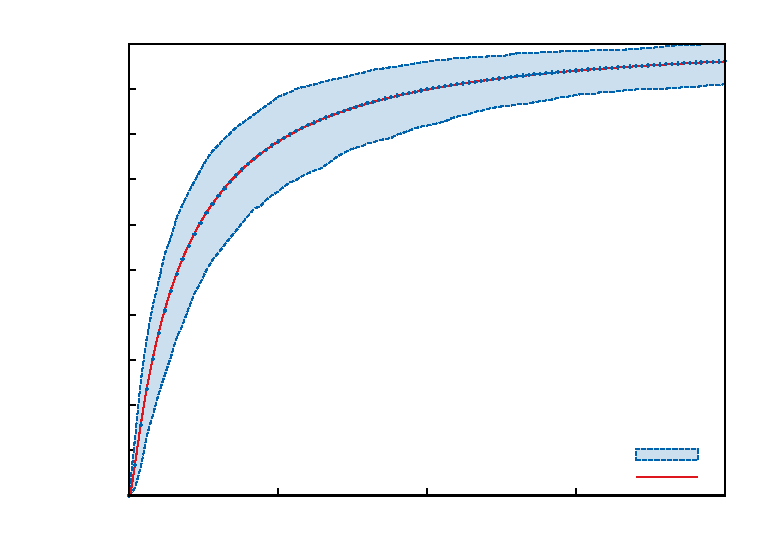
\includegraphics{./figures/elkc_exp_1D_lognormal_1}}%
    \gplfronttext
  \end{picture}%
\endgroup
}}\hspace*{\fill}
  \caption{Expectation of LKC for $\Msize=100$, $\mean=0.5$, $\std^2=2$, $\Lc=0.5$, and $\HS=\zu$ (log-normal distribution with cumulative hitting set) in 1D. Experimental results are calculated over $1\,000$ realizations.}
\end{figure}

\newpage 
\subsubsection{Two dimensions}
\begin{subequations}
\begin{align}
  &\Expec\left\{\LKC_0^\ES\right\} = \frac{\SpecMom}{2\pi}\LKC_2^\MRF\GMFk_2 + \sqrt{\frac{\SpecMom}{2\pi}}\LKC_1^\MRF\GMFk_1 + \LKC_0^\MRF\GMFk_0\\
  &\Expec\left\{\LKC_1^\ES\right\} = \sqrt{\frac{\SpecMom\pi}{8}}\LKC_2^\MRF\GMFk_1 + \LKC_1^\MRF\GMFk_0\\
  &\Expec\left\{\LKC_2^\ES\right\} = \LKC_2^\MRF\GMFk_0
\end{align}
\end{subequations}


\begin{figure}[!h]
  \centering
  \hspace*{\fill}
  \subfigure{\scalebox{0.5}{% GNUPLOT: LaTeX picture with Postscript
\begingroup
  \makeatletter
  \providecommand\color[2][]{%
    \GenericError{(gnuplot) \space\space\space\@spaces}{%
      Package color not loaded in conjunction with
      terminal option `colourtext'%
    }{See the gnuplot documentation for explanation.%
    }{Either use 'blacktext' in gnuplot or load the package
      color.sty in LaTeX.}%
    \renewcommand\color[2][]{}%
  }%
  \providecommand\includegraphics[2][]{%
    \GenericError{(gnuplot) \space\space\space\@spaces}{%
      Package graphicx or graphics not loaded%
    }{See the gnuplot documentation for explanation.%
    }{The gnuplot epslatex terminal needs graphicx.sty or graphics.sty.}%
    \renewcommand\includegraphics[2][]{}%
  }%
  \providecommand\rotatebox[2]{#2}%
  \@ifundefined{ifGPcolor}{%
    \newif\ifGPcolor
    \GPcolorfalse
  }{}%
  \@ifundefined{ifGPblacktext}{%
    \newif\ifGPblacktext
    \GPblacktexttrue
  }{}%
  % define a \g@addto@macro without @ in the name:
  \let\gplgaddtomacro\g@addto@macro
  % define empty templates for all commands taking text:
  \gdef\gplbacktext{}%
  \gdef\gplfronttext{}%
  \makeatother
  \ifGPblacktext
    % no textcolor at all
    \def\colorrgb#1{}%
    \def\colorgray#1{}%
  \else
    % gray or color?
    \ifGPcolor
      \def\colorrgb#1{\color[rgb]{#1}}%
      \def\colorgray#1{\color[gray]{#1}}%
      \expandafter\def\csname LTw\endcsname{\color{white}}%
      \expandafter\def\csname LTb\endcsname{\color{black}}%
      \expandafter\def\csname LTa\endcsname{\color{black}}%
      \expandafter\def\csname LT0\endcsname{\color[rgb]{1,0,0}}%
      \expandafter\def\csname LT1\endcsname{\color[rgb]{0,1,0}}%
      \expandafter\def\csname LT2\endcsname{\color[rgb]{0,0,1}}%
      \expandafter\def\csname LT3\endcsname{\color[rgb]{1,0,1}}%
      \expandafter\def\csname LT4\endcsname{\color[rgb]{0,1,1}}%
      \expandafter\def\csname LT5\endcsname{\color[rgb]{1,1,0}}%
      \expandafter\def\csname LT6\endcsname{\color[rgb]{0,0,0}}%
      \expandafter\def\csname LT7\endcsname{\color[rgb]{1,0.3,0}}%
      \expandafter\def\csname LT8\endcsname{\color[rgb]{0.5,0.5,0.5}}%
    \else
      % gray
      \def\colorrgb#1{\color{black}}%
      \def\colorgray#1{\color[gray]{#1}}%
      \expandafter\def\csname LTw\endcsname{\color{white}}%
      \expandafter\def\csname LTb\endcsname{\color{black}}%
      \expandafter\def\csname LTa\endcsname{\color{black}}%
      \expandafter\def\csname LT0\endcsname{\color{black}}%
      \expandafter\def\csname LT1\endcsname{\color{black}}%
      \expandafter\def\csname LT2\endcsname{\color{black}}%
      \expandafter\def\csname LT3\endcsname{\color{black}}%
      \expandafter\def\csname LT4\endcsname{\color{black}}%
      \expandafter\def\csname LT5\endcsname{\color{black}}%
      \expandafter\def\csname LT6\endcsname{\color{black}}%
      \expandafter\def\csname LT7\endcsname{\color{black}}%
      \expandafter\def\csname LT8\endcsname{\color{black}}%
    \fi
  \fi
  \setlength{\unitlength}{0.0500bp}%
  \begin{picture}(7200.00,5040.00)%
    \gplgaddtomacro\gplbacktext{%
      \csname LTb\endcsname%
      \put(814,704){\makebox(0,0)[r]{\strut{}-40}}%
      \put(814,1111){\makebox(0,0)[r]{\strut{}-30}}%
      \put(814,1518){\makebox(0,0)[r]{\strut{}-20}}%
      \put(814,1925){\makebox(0,0)[r]{\strut{}-10}}%
      \put(814,2332){\makebox(0,0)[r]{\strut{} 0}}%
      \put(814,2740){\makebox(0,0)[r]{\strut{} 10}}%
      \put(814,3147){\makebox(0,0)[r]{\strut{} 20}}%
      \put(814,3554){\makebox(0,0)[r]{\strut{} 30}}%
      \put(814,3961){\makebox(0,0)[r]{\strut{} 40}}%
      \put(814,4368){\makebox(0,0)[r]{\strut{} 50}}%
      \put(814,4775){\makebox(0,0)[r]{\strut{} 60}}%
      \put(946,484){\makebox(0,0){\strut{}-4}}%
      \put(1678,484){\makebox(0,0){\strut{}-3}}%
      \put(2410,484){\makebox(0,0){\strut{}-2}}%
      \put(3142,484){\makebox(0,0){\strut{}-1}}%
      \put(3875,484){\makebox(0,0){\strut{} 0}}%
      \put(4607,484){\makebox(0,0){\strut{} 1}}%
      \put(5339,484){\makebox(0,0){\strut{} 2}}%
      \put(6071,484){\makebox(0,0){\strut{} 3}}%
      \put(6803,484){\makebox(0,0){\strut{} 4}}%
      \csname LTb\endcsname%
      \put(176,2739){\rotatebox{90}{\makebox(0,0){\strut{}Euler characteristic}}}%
      \put(3874,154){\makebox(0,0){\strut{}$\lset$}}%
    }%
    \gplgaddtomacro\gplfronttext{%
      \csname LTb\endcsname%
      \put(2662,4602){\makebox(0,0)[r]{\strut{}Experimental}}%
      \csname LTb\endcsname%
      \put(2662,4382){\makebox(0,0)[r]{\strut{}Theoretical}}%
    }%
    \gplbacktext
    \put(0,0){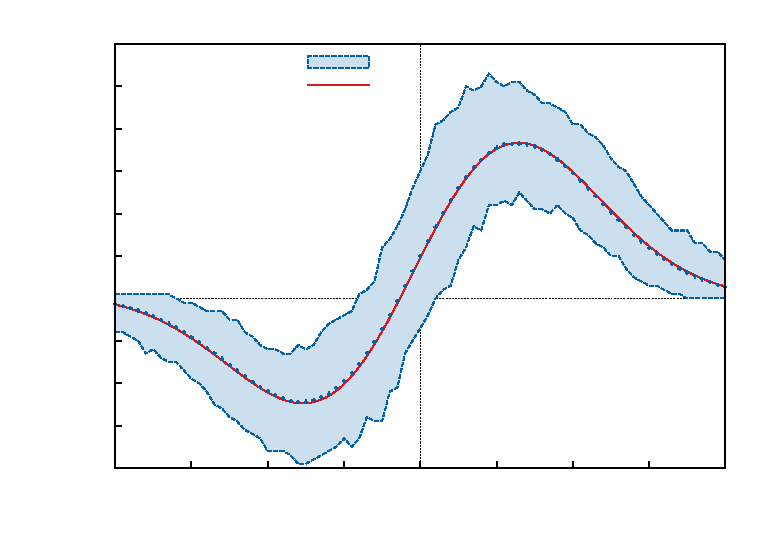
\includegraphics{./figures/elkc_exp_2D_gaussian_0}}%
    \gplfronttext
  \end{picture}%
\endgroup
}}\hfill
  \subfigure{\scalebox{0.5}{% GNUPLOT: LaTeX picture with Postscript
\begingroup
  \makeatletter
  \providecommand\color[2][]{%
    \GenericError{(gnuplot) \space\space\space\@spaces}{%
      Package color not loaded in conjunction with
      terminal option `colourtext'%
    }{See the gnuplot documentation for explanation.%
    }{Either use 'blacktext' in gnuplot or load the package
      color.sty in LaTeX.}%
    \renewcommand\color[2][]{}%
  }%
  \providecommand\includegraphics[2][]{%
    \GenericError{(gnuplot) \space\space\space\@spaces}{%
      Package graphicx or graphics not loaded%
    }{See the gnuplot documentation for explanation.%
    }{The gnuplot epslatex terminal needs graphicx.sty or graphics.sty.}%
    \renewcommand\includegraphics[2][]{}%
  }%
  \providecommand\rotatebox[2]{#2}%
  \@ifundefined{ifGPcolor}{%
    \newif\ifGPcolor
    \GPcolorfalse
  }{}%
  \@ifundefined{ifGPblacktext}{%
    \newif\ifGPblacktext
    \GPblacktexttrue
  }{}%
  % define a \g@addto@macro without @ in the name:
  \let\gplgaddtomacro\g@addto@macro
  % define empty templates for all commands taking text:
  \gdef\gplbacktext{}%
  \gdef\gplfronttext{}%
  \makeatother
  \ifGPblacktext
    % no textcolor at all
    \def\colorrgb#1{}%
    \def\colorgray#1{}%
  \else
    % gray or color?
    \ifGPcolor
      \def\colorrgb#1{\color[rgb]{#1}}%
      \def\colorgray#1{\color[gray]{#1}}%
      \expandafter\def\csname LTw\endcsname{\color{white}}%
      \expandafter\def\csname LTb\endcsname{\color{black}}%
      \expandafter\def\csname LTa\endcsname{\color{black}}%
      \expandafter\def\csname LT0\endcsname{\color[rgb]{1,0,0}}%
      \expandafter\def\csname LT1\endcsname{\color[rgb]{0,1,0}}%
      \expandafter\def\csname LT2\endcsname{\color[rgb]{0,0,1}}%
      \expandafter\def\csname LT3\endcsname{\color[rgb]{1,0,1}}%
      \expandafter\def\csname LT4\endcsname{\color[rgb]{0,1,1}}%
      \expandafter\def\csname LT5\endcsname{\color[rgb]{1,1,0}}%
      \expandafter\def\csname LT6\endcsname{\color[rgb]{0,0,0}}%
      \expandafter\def\csname LT7\endcsname{\color[rgb]{1,0.3,0}}%
      \expandafter\def\csname LT8\endcsname{\color[rgb]{0.5,0.5,0.5}}%
    \else
      % gray
      \def\colorrgb#1{\color{black}}%
      \def\colorgray#1{\color[gray]{#1}}%
      \expandafter\def\csname LTw\endcsname{\color{white}}%
      \expandafter\def\csname LTb\endcsname{\color{black}}%
      \expandafter\def\csname LTa\endcsname{\color{black}}%
      \expandafter\def\csname LT0\endcsname{\color{black}}%
      \expandafter\def\csname LT1\endcsname{\color{black}}%
      \expandafter\def\csname LT2\endcsname{\color{black}}%
      \expandafter\def\csname LT3\endcsname{\color{black}}%
      \expandafter\def\csname LT4\endcsname{\color{black}}%
      \expandafter\def\csname LT5\endcsname{\color{black}}%
      \expandafter\def\csname LT6\endcsname{\color{black}}%
      \expandafter\def\csname LT7\endcsname{\color{black}}%
      \expandafter\def\csname LT8\endcsname{\color{black}}%
    \fi
  \fi
  \setlength{\unitlength}{0.0500bp}%
  \begin{picture}(7200.00,5040.00)%
    \gplgaddtomacro\gplbacktext{%
      \csname LTb\endcsname%
      \put(946,704){\makebox(0,0)[r]{\strut{} 0}}%
      \put(946,1156){\makebox(0,0)[r]{\strut{} 100}}%
      \put(946,1609){\makebox(0,0)[r]{\strut{} 200}}%
      \put(946,2061){\makebox(0,0)[r]{\strut{} 300}}%
      \put(946,2513){\makebox(0,0)[r]{\strut{} 400}}%
      \put(946,2966){\makebox(0,0)[r]{\strut{} 500}}%
      \put(946,3418){\makebox(0,0)[r]{\strut{} 600}}%
      \put(946,3870){\makebox(0,0)[r]{\strut{} 700}}%
      \put(946,4323){\makebox(0,0)[r]{\strut{} 800}}%
      \put(946,4775){\makebox(0,0)[r]{\strut{} 900}}%
      \put(1078,484){\makebox(0,0){\strut{}-4}}%
      \put(1794,484){\makebox(0,0){\strut{}-3}}%
      \put(2509,484){\makebox(0,0){\strut{}-2}}%
      \put(3225,484){\makebox(0,0){\strut{}-1}}%
      \put(3941,484){\makebox(0,0){\strut{} 0}}%
      \put(4656,484){\makebox(0,0){\strut{} 1}}%
      \put(5372,484){\makebox(0,0){\strut{} 2}}%
      \put(6087,484){\makebox(0,0){\strut{} 3}}%
      \put(6803,484){\makebox(0,0){\strut{} 4}}%
      \csname LTb\endcsname%
      \put(176,2739){\rotatebox{90}{\makebox(0,0){\strut{}Half diameter}}}%
      \put(3940,154){\makebox(0,0){\strut{}$\lset$}}%
    }%
    \gplgaddtomacro\gplfronttext{%
      \csname LTb\endcsname%
      \put(5816,4602){\makebox(0,0)[r]{\strut{}Theoretical}}%
    }%
    \gplbacktext
    \put(0,0){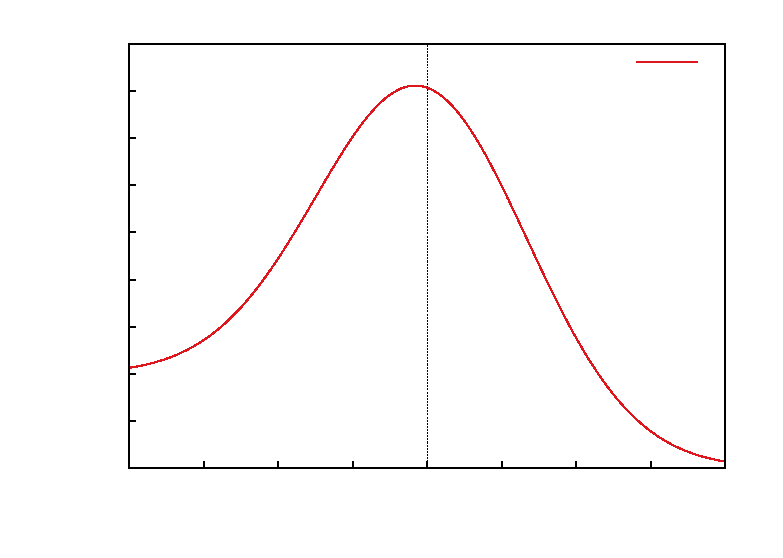
\includegraphics{./figures/elkc_exp_2D_gaussian_1}}%
    \gplfronttext
  \end{picture}%
\endgroup
}}\hfill
  \subfigure{\scalebox{0.5}{% GNUPLOT: LaTeX picture with Postscript
\begingroup
  \makeatletter
  \providecommand\color[2][]{%
    \GenericError{(gnuplot) \space\space\space\@spaces}{%
      Package color not loaded in conjunction with
      terminal option `colourtext'%
    }{See the gnuplot documentation for explanation.%
    }{Either use 'blacktext' in gnuplot or load the package
      color.sty in LaTeX.}%
    \renewcommand\color[2][]{}%
  }%
  \providecommand\includegraphics[2][]{%
    \GenericError{(gnuplot) \space\space\space\@spaces}{%
      Package graphicx or graphics not loaded%
    }{See the gnuplot documentation for explanation.%
    }{The gnuplot epslatex terminal needs graphicx.sty or graphics.sty.}%
    \renewcommand\includegraphics[2][]{}%
  }%
  \providecommand\rotatebox[2]{#2}%
  \@ifundefined{ifGPcolor}{%
    \newif\ifGPcolor
    \GPcolorfalse
  }{}%
  \@ifundefined{ifGPblacktext}{%
    \newif\ifGPblacktext
    \GPblacktexttrue
  }{}%
  % define a \g@addto@macro without @ in the name:
  \let\gplgaddtomacro\g@addto@macro
  % define empty templates for all commands taking text:
  \gdef\gplbacktext{}%
  \gdef\gplfronttext{}%
  \makeatother
  \ifGPblacktext
    % no textcolor at all
    \def\colorrgb#1{}%
    \def\colorgray#1{}%
  \else
    % gray or color?
    \ifGPcolor
      \def\colorrgb#1{\color[rgb]{#1}}%
      \def\colorgray#1{\color[gray]{#1}}%
      \expandafter\def\csname LTw\endcsname{\color{white}}%
      \expandafter\def\csname LTb\endcsname{\color{black}}%
      \expandafter\def\csname LTa\endcsname{\color{black}}%
      \expandafter\def\csname LT0\endcsname{\color[rgb]{1,0,0}}%
      \expandafter\def\csname LT1\endcsname{\color[rgb]{0,1,0}}%
      \expandafter\def\csname LT2\endcsname{\color[rgb]{0,0,1}}%
      \expandafter\def\csname LT3\endcsname{\color[rgb]{1,0,1}}%
      \expandafter\def\csname LT4\endcsname{\color[rgb]{0,1,1}}%
      \expandafter\def\csname LT5\endcsname{\color[rgb]{1,1,0}}%
      \expandafter\def\csname LT6\endcsname{\color[rgb]{0,0,0}}%
      \expandafter\def\csname LT7\endcsname{\color[rgb]{1,0.3,0}}%
      \expandafter\def\csname LT8\endcsname{\color[rgb]{0.5,0.5,0.5}}%
    \else
      % gray
      \def\colorrgb#1{\color{black}}%
      \def\colorgray#1{\color[gray]{#1}}%
      \expandafter\def\csname LTw\endcsname{\color{white}}%
      \expandafter\def\csname LTb\endcsname{\color{black}}%
      \expandafter\def\csname LTa\endcsname{\color{black}}%
      \expandafter\def\csname LT0\endcsname{\color{black}}%
      \expandafter\def\csname LT1\endcsname{\color{black}}%
      \expandafter\def\csname LT2\endcsname{\color{black}}%
      \expandafter\def\csname LT3\endcsname{\color{black}}%
      \expandafter\def\csname LT4\endcsname{\color{black}}%
      \expandafter\def\csname LT5\endcsname{\color{black}}%
      \expandafter\def\csname LT6\endcsname{\color{black}}%
      \expandafter\def\csname LT7\endcsname{\color{black}}%
      \expandafter\def\csname LT8\endcsname{\color{black}}%
    \fi
  \fi
  \setlength{\unitlength}{0.0500bp}%
  \begin{picture}(7200.00,5040.00)%
    \gplgaddtomacro\gplbacktext{%
      \csname LTb\endcsname%
      \put(1210,704){\makebox(0,0)[r]{\strut{} 0}}%
      \put(1210,1518){\makebox(0,0)[r]{\strut{} 2000}}%
      \put(1210,2332){\makebox(0,0)[r]{\strut{} 4000}}%
      \put(1210,3147){\makebox(0,0)[r]{\strut{} 6000}}%
      \put(1210,3961){\makebox(0,0)[r]{\strut{} 8000}}%
      \put(1210,4775){\makebox(0,0)[r]{\strut{} 10000}}%
      \put(1342,484){\makebox(0,0){\strut{}-4}}%
      \put(2025,484){\makebox(0,0){\strut{}-3}}%
      \put(2707,484){\makebox(0,0){\strut{}-2}}%
      \put(3390,484){\makebox(0,0){\strut{}-1}}%
      \put(4073,484){\makebox(0,0){\strut{} 0}}%
      \put(4755,484){\makebox(0,0){\strut{} 1}}%
      \put(5438,484){\makebox(0,0){\strut{} 2}}%
      \put(6120,484){\makebox(0,0){\strut{} 3}}%
      \put(6803,484){\makebox(0,0){\strut{} 4}}%
      \csname LTb\endcsname%
      \put(176,2739){\rotatebox{90}{\makebox(0,0){\strut{}Surface area}}}%
      \put(4072,154){\makebox(0,0){\strut{}$\lset$}}%
    }%
    \gplgaddtomacro\gplfronttext{%
      \csname LTb\endcsname%
      \put(5816,4602){\makebox(0,0)[r]{\strut{}Experimental}}%
      \csname LTb\endcsname%
      \put(5816,4382){\makebox(0,0)[r]{\strut{}Theoretical}}%
    }%
    \gplbacktext
    \put(0,0){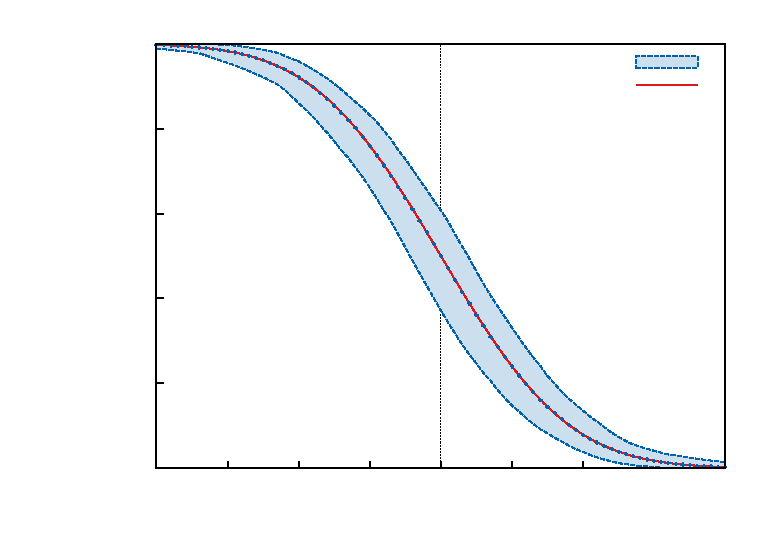
\includegraphics{./figures/elkc_exp_2D_gaussian_2}}%
    \gplfronttext
  \end{picture}%
\endgroup
}}\hspace*{\fill}
  \caption{Expectation of LKC for $\Msize=100$, $\mean=0.0$, $\std^2=2$, $\Lc=5$, and $\HS=\uinf$ (gaussian distribution with tail hitting set) in 2D. Experimental results are calculated over $1\,000$ realizations.}
\end{figure}

\begin{figure}[!h]
  \centering
  \hspace*{\fill}
  \subfigure{\scalebox{0.5}{% GNUPLOT: LaTeX picture with Postscript
\begingroup
  \makeatletter
  \providecommand\color[2][]{%
    \GenericError{(gnuplot) \space\space\space\@spaces}{%
      Package color not loaded in conjunction with
      terminal option `colourtext'%
    }{See the gnuplot documentation for explanation.%
    }{Either use 'blacktext' in gnuplot or load the package
      color.sty in LaTeX.}%
    \renewcommand\color[2][]{}%
  }%
  \providecommand\includegraphics[2][]{%
    \GenericError{(gnuplot) \space\space\space\@spaces}{%
      Package graphicx or graphics not loaded%
    }{See the gnuplot documentation for explanation.%
    }{The gnuplot epslatex terminal needs graphicx.sty or graphics.sty.}%
    \renewcommand\includegraphics[2][]{}%
  }%
  \providecommand\rotatebox[2]{#2}%
  \@ifundefined{ifGPcolor}{%
    \newif\ifGPcolor
    \GPcolorfalse
  }{}%
  \@ifundefined{ifGPblacktext}{%
    \newif\ifGPblacktext
    \GPblacktexttrue
  }{}%
  % define a \g@addto@macro without @ in the name:
  \let\gplgaddtomacro\g@addto@macro
  % define empty templates for all commands taking text:
  \gdef\gplbacktext{}%
  \gdef\gplfronttext{}%
  \makeatother
  \ifGPblacktext
    % no textcolor at all
    \def\colorrgb#1{}%
    \def\colorgray#1{}%
  \else
    % gray or color?
    \ifGPcolor
      \def\colorrgb#1{\color[rgb]{#1}}%
      \def\colorgray#1{\color[gray]{#1}}%
      \expandafter\def\csname LTw\endcsname{\color{white}}%
      \expandafter\def\csname LTb\endcsname{\color{black}}%
      \expandafter\def\csname LTa\endcsname{\color{black}}%
      \expandafter\def\csname LT0\endcsname{\color[rgb]{1,0,0}}%
      \expandafter\def\csname LT1\endcsname{\color[rgb]{0,1,0}}%
      \expandafter\def\csname LT2\endcsname{\color[rgb]{0,0,1}}%
      \expandafter\def\csname LT3\endcsname{\color[rgb]{1,0,1}}%
      \expandafter\def\csname LT4\endcsname{\color[rgb]{0,1,1}}%
      \expandafter\def\csname LT5\endcsname{\color[rgb]{1,1,0}}%
      \expandafter\def\csname LT6\endcsname{\color[rgb]{0,0,0}}%
      \expandafter\def\csname LT7\endcsname{\color[rgb]{1,0.3,0}}%
      \expandafter\def\csname LT8\endcsname{\color[rgb]{0.5,0.5,0.5}}%
    \else
      % gray
      \def\colorrgb#1{\color{black}}%
      \def\colorgray#1{\color[gray]{#1}}%
      \expandafter\def\csname LTw\endcsname{\color{white}}%
      \expandafter\def\csname LTb\endcsname{\color{black}}%
      \expandafter\def\csname LTa\endcsname{\color{black}}%
      \expandafter\def\csname LT0\endcsname{\color{black}}%
      \expandafter\def\csname LT1\endcsname{\color{black}}%
      \expandafter\def\csname LT2\endcsname{\color{black}}%
      \expandafter\def\csname LT3\endcsname{\color{black}}%
      \expandafter\def\csname LT4\endcsname{\color{black}}%
      \expandafter\def\csname LT5\endcsname{\color{black}}%
      \expandafter\def\csname LT6\endcsname{\color{black}}%
      \expandafter\def\csname LT7\endcsname{\color{black}}%
      \expandafter\def\csname LT8\endcsname{\color{black}}%
    \fi
  \fi
  \setlength{\unitlength}{0.0500bp}%
  \begin{picture}(7200.00,5040.00)%
    \gplgaddtomacro\gplbacktext{%
      \csname LTb\endcsname%
      \put(814,704){\makebox(0,0)[r]{\strut{}-40}}%
      \put(814,1111){\makebox(0,0)[r]{\strut{}-30}}%
      \put(814,1518){\makebox(0,0)[r]{\strut{}-20}}%
      \put(814,1925){\makebox(0,0)[r]{\strut{}-10}}%
      \put(814,2332){\makebox(0,0)[r]{\strut{} 0}}%
      \put(814,2740){\makebox(0,0)[r]{\strut{} 10}}%
      \put(814,3147){\makebox(0,0)[r]{\strut{} 20}}%
      \put(814,3554){\makebox(0,0)[r]{\strut{} 30}}%
      \put(814,3961){\makebox(0,0)[r]{\strut{} 40}}%
      \put(814,4368){\makebox(0,0)[r]{\strut{} 50}}%
      \put(814,4775){\makebox(0,0)[r]{\strut{} 60}}%
      \put(946,484){\makebox(0,0){\strut{} 0.01}}%
      \put(2117,484){\makebox(0,0){\strut{} 0.1}}%
      \put(3289,484){\makebox(0,0){\strut{} 1}}%
      \put(4460,484){\makebox(0,0){\strut{} 10}}%
      \put(5632,484){\makebox(0,0){\strut{} 100}}%
      \put(6803,484){\makebox(0,0){\strut{} 1000}}%
      \csname LTb\endcsname%
      \put(176,2739){\rotatebox{90}{\makebox(0,0){\strut{}Euler characteristic}}}%
      \put(3874,154){\makebox(0,0){\strut{}$\lset$}}%
    }%
    \gplgaddtomacro\gplfronttext{%
      \csname LTb\endcsname%
      \put(5816,4602){\makebox(0,0)[r]{\strut{}Experimental}}%
      \csname LTb\endcsname%
      \put(5816,4382){\makebox(0,0)[r]{\strut{}Theoretical}}%
    }%
    \gplbacktext
    \put(0,0){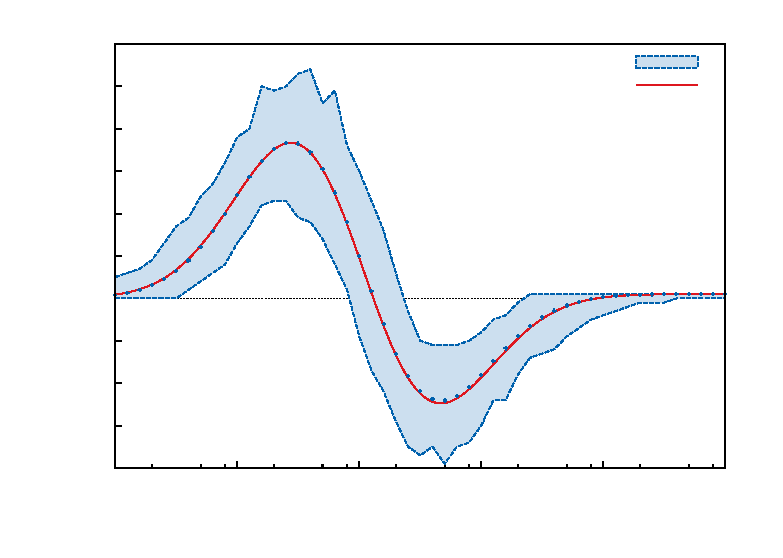
\includegraphics{./figures/elkc_exp_2D_lognormal_0}}%
    \gplfronttext
  \end{picture}%
\endgroup
}}\hfill
  \subfigure{\scalebox{0.5}{% GNUPLOT: LaTeX picture with Postscript
\begingroup
  \makeatletter
  \providecommand\color[2][]{%
    \GenericError{(gnuplot) \space\space\space\@spaces}{%
      Package color not loaded in conjunction with
      terminal option `colourtext'%
    }{See the gnuplot documentation for explanation.%
    }{Either use 'blacktext' in gnuplot or load the package
      color.sty in LaTeX.}%
    \renewcommand\color[2][]{}%
  }%
  \providecommand\includegraphics[2][]{%
    \GenericError{(gnuplot) \space\space\space\@spaces}{%
      Package graphicx or graphics not loaded%
    }{See the gnuplot documentation for explanation.%
    }{The gnuplot epslatex terminal needs graphicx.sty or graphics.sty.}%
    \renewcommand\includegraphics[2][]{}%
  }%
  \providecommand\rotatebox[2]{#2}%
  \@ifundefined{ifGPcolor}{%
    \newif\ifGPcolor
    \GPcolorfalse
  }{}%
  \@ifundefined{ifGPblacktext}{%
    \newif\ifGPblacktext
    \GPblacktexttrue
  }{}%
  % define a \g@addto@macro without @ in the name:
  \let\gplgaddtomacro\g@addto@macro
  % define empty templates for all commands taking text:
  \gdef\gplbacktext{}%
  \gdef\gplfronttext{}%
  \makeatother
  \ifGPblacktext
    % no textcolor at all
    \def\colorrgb#1{}%
    \def\colorgray#1{}%
  \else
    % gray or color?
    \ifGPcolor
      \def\colorrgb#1{\color[rgb]{#1}}%
      \def\colorgray#1{\color[gray]{#1}}%
      \expandafter\def\csname LTw\endcsname{\color{white}}%
      \expandafter\def\csname LTb\endcsname{\color{black}}%
      \expandafter\def\csname LTa\endcsname{\color{black}}%
      \expandafter\def\csname LT0\endcsname{\color[rgb]{1,0,0}}%
      \expandafter\def\csname LT1\endcsname{\color[rgb]{0,1,0}}%
      \expandafter\def\csname LT2\endcsname{\color[rgb]{0,0,1}}%
      \expandafter\def\csname LT3\endcsname{\color[rgb]{1,0,1}}%
      \expandafter\def\csname LT4\endcsname{\color[rgb]{0,1,1}}%
      \expandafter\def\csname LT5\endcsname{\color[rgb]{1,1,0}}%
      \expandafter\def\csname LT6\endcsname{\color[rgb]{0,0,0}}%
      \expandafter\def\csname LT7\endcsname{\color[rgb]{1,0.3,0}}%
      \expandafter\def\csname LT8\endcsname{\color[rgb]{0.5,0.5,0.5}}%
    \else
      % gray
      \def\colorrgb#1{\color{black}}%
      \def\colorgray#1{\color[gray]{#1}}%
      \expandafter\def\csname LTw\endcsname{\color{white}}%
      \expandafter\def\csname LTb\endcsname{\color{black}}%
      \expandafter\def\csname LTa\endcsname{\color{black}}%
      \expandafter\def\csname LT0\endcsname{\color{black}}%
      \expandafter\def\csname LT1\endcsname{\color{black}}%
      \expandafter\def\csname LT2\endcsname{\color{black}}%
      \expandafter\def\csname LT3\endcsname{\color{black}}%
      \expandafter\def\csname LT4\endcsname{\color{black}}%
      \expandafter\def\csname LT5\endcsname{\color{black}}%
      \expandafter\def\csname LT6\endcsname{\color{black}}%
      \expandafter\def\csname LT7\endcsname{\color{black}}%
      \expandafter\def\csname LT8\endcsname{\color{black}}%
    \fi
  \fi
  \setlength{\unitlength}{0.0500bp}%
  \begin{picture}(7200.00,5040.00)%
    \gplgaddtomacro\gplbacktext{%
      \csname LTb\endcsname%
      \put(946,704){\makebox(0,0)[r]{\strut{} 0}}%
      \put(946,1156){\makebox(0,0)[r]{\strut{} 100}}%
      \put(946,1609){\makebox(0,0)[r]{\strut{} 200}}%
      \put(946,2061){\makebox(0,0)[r]{\strut{} 300}}%
      \put(946,2513){\makebox(0,0)[r]{\strut{} 400}}%
      \put(946,2966){\makebox(0,0)[r]{\strut{} 500}}%
      \put(946,3418){\makebox(0,0)[r]{\strut{} 600}}%
      \put(946,3870){\makebox(0,0)[r]{\strut{} 700}}%
      \put(946,4323){\makebox(0,0)[r]{\strut{} 800}}%
      \put(946,4775){\makebox(0,0)[r]{\strut{} 900}}%
      \put(1078,484){\makebox(0,0){\strut{} 0.01}}%
      \put(2223,484){\makebox(0,0){\strut{} 0.1}}%
      \put(3368,484){\makebox(0,0){\strut{} 1}}%
      \put(4513,484){\makebox(0,0){\strut{} 10}}%
      \put(5658,484){\makebox(0,0){\strut{} 100}}%
      \put(6803,484){\makebox(0,0){\strut{} 1000}}%
      \csname LTb\endcsname%
      \put(176,2739){\rotatebox{90}{\makebox(0,0){\strut{}Half diameter}}}%
      \put(3940,154){\makebox(0,0){\strut{}$\lset$}}%
    }%
    \gplgaddtomacro\gplfronttext{%
      \csname LTb\endcsname%
      \put(5816,4602){\makebox(0,0)[r]{\strut{}Theoretical}}%
    }%
    \gplbacktext
    \put(0,0){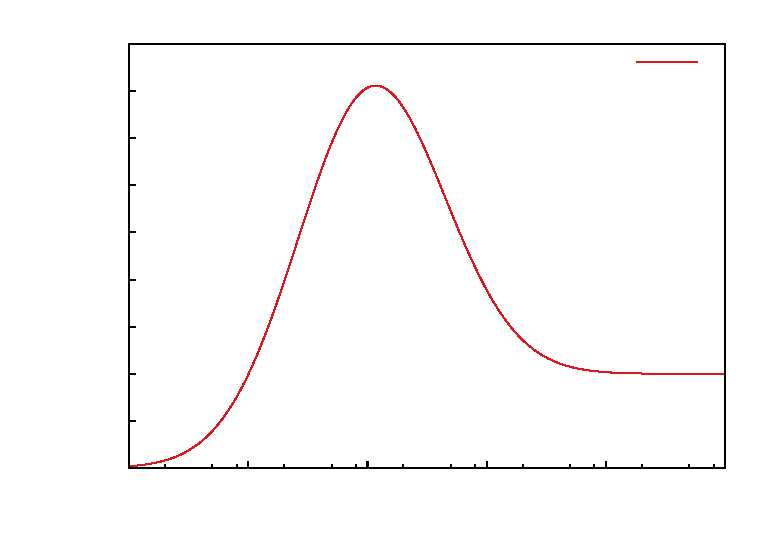
\includegraphics{./figures/elkc_exp_2D_lognormal_1}}%
    \gplfronttext
  \end{picture}%
\endgroup
}}\hfill
  \subfigure{\scalebox{0.5}{% GNUPLOT: LaTeX picture with Postscript
\begingroup
  \makeatletter
  \providecommand\color[2][]{%
    \GenericError{(gnuplot) \space\space\space\@spaces}{%
      Package color not loaded in conjunction with
      terminal option `colourtext'%
    }{See the gnuplot documentation for explanation.%
    }{Either use 'blacktext' in gnuplot or load the package
      color.sty in LaTeX.}%
    \renewcommand\color[2][]{}%
  }%
  \providecommand\includegraphics[2][]{%
    \GenericError{(gnuplot) \space\space\space\@spaces}{%
      Package graphicx or graphics not loaded%
    }{See the gnuplot documentation for explanation.%
    }{The gnuplot epslatex terminal needs graphicx.sty or graphics.sty.}%
    \renewcommand\includegraphics[2][]{}%
  }%
  \providecommand\rotatebox[2]{#2}%
  \@ifundefined{ifGPcolor}{%
    \newif\ifGPcolor
    \GPcolorfalse
  }{}%
  \@ifundefined{ifGPblacktext}{%
    \newif\ifGPblacktext
    \GPblacktexttrue
  }{}%
  % define a \g@addto@macro without @ in the name:
  \let\gplgaddtomacro\g@addto@macro
  % define empty templates for all commands taking text:
  \gdef\gplbacktext{}%
  \gdef\gplfronttext{}%
  \makeatother
  \ifGPblacktext
    % no textcolor at all
    \def\colorrgb#1{}%
    \def\colorgray#1{}%
  \else
    % gray or color?
    \ifGPcolor
      \def\colorrgb#1{\color[rgb]{#1}}%
      \def\colorgray#1{\color[gray]{#1}}%
      \expandafter\def\csname LTw\endcsname{\color{white}}%
      \expandafter\def\csname LTb\endcsname{\color{black}}%
      \expandafter\def\csname LTa\endcsname{\color{black}}%
      \expandafter\def\csname LT0\endcsname{\color[rgb]{1,0,0}}%
      \expandafter\def\csname LT1\endcsname{\color[rgb]{0,1,0}}%
      \expandafter\def\csname LT2\endcsname{\color[rgb]{0,0,1}}%
      \expandafter\def\csname LT3\endcsname{\color[rgb]{1,0,1}}%
      \expandafter\def\csname LT4\endcsname{\color[rgb]{0,1,1}}%
      \expandafter\def\csname LT5\endcsname{\color[rgb]{1,1,0}}%
      \expandafter\def\csname LT6\endcsname{\color[rgb]{0,0,0}}%
      \expandafter\def\csname LT7\endcsname{\color[rgb]{1,0.3,0}}%
      \expandafter\def\csname LT8\endcsname{\color[rgb]{0.5,0.5,0.5}}%
    \else
      % gray
      \def\colorrgb#1{\color{black}}%
      \def\colorgray#1{\color[gray]{#1}}%
      \expandafter\def\csname LTw\endcsname{\color{white}}%
      \expandafter\def\csname LTb\endcsname{\color{black}}%
      \expandafter\def\csname LTa\endcsname{\color{black}}%
      \expandafter\def\csname LT0\endcsname{\color{black}}%
      \expandafter\def\csname LT1\endcsname{\color{black}}%
      \expandafter\def\csname LT2\endcsname{\color{black}}%
      \expandafter\def\csname LT3\endcsname{\color{black}}%
      \expandafter\def\csname LT4\endcsname{\color{black}}%
      \expandafter\def\csname LT5\endcsname{\color{black}}%
      \expandafter\def\csname LT6\endcsname{\color{black}}%
      \expandafter\def\csname LT7\endcsname{\color{black}}%
      \expandafter\def\csname LT8\endcsname{\color{black}}%
    \fi
  \fi
  \setlength{\unitlength}{0.0500bp}%
  \begin{picture}(7200.00,5040.00)%
    \gplgaddtomacro\gplbacktext{%
      \csname LTb\endcsname%
      \put(1210,704){\makebox(0,0)[r]{\strut{} 0}}%
      \put(1210,1518){\makebox(0,0)[r]{\strut{} 2000}}%
      \put(1210,2332){\makebox(0,0)[r]{\strut{} 4000}}%
      \put(1210,3147){\makebox(0,0)[r]{\strut{} 6000}}%
      \put(1210,3961){\makebox(0,0)[r]{\strut{} 8000}}%
      \put(1210,4775){\makebox(0,0)[r]{\strut{} 10000}}%
      \put(1342,484){\makebox(0,0){\strut{} 0.01}}%
      \put(2434,484){\makebox(0,0){\strut{} 0.1}}%
      \put(3526,484){\makebox(0,0){\strut{} 1}}%
      \put(4619,484){\makebox(0,0){\strut{} 10}}%
      \put(5711,484){\makebox(0,0){\strut{} 100}}%
      \put(6803,484){\makebox(0,0){\strut{} 1000}}%
      \csname LTb\endcsname%
      \put(176,2739){\rotatebox{90}{\makebox(0,0){\strut{}Surface area}}}%
      \put(4072,154){\makebox(0,0){\strut{}$\lset$}}%
    }%
    \gplgaddtomacro\gplfronttext{%
      \csname LTb\endcsname%
      \put(3058,4602){\makebox(0,0)[r]{\strut{}Experimental}}%
      \csname LTb\endcsname%
      \put(3058,4382){\makebox(0,0)[r]{\strut{}Theoretical}}%
    }%
    \gplbacktext
    \put(0,0){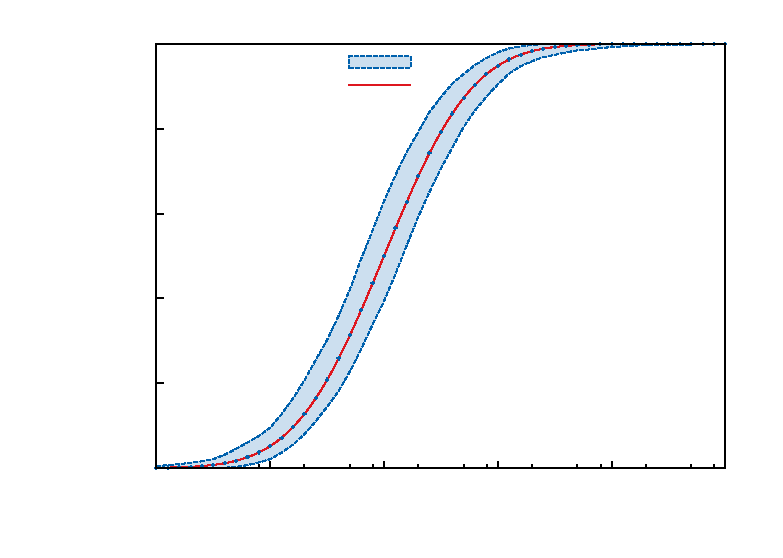
\includegraphics{./figures/elkc_exp_2D_lognormal_2}}%
    \gplfronttext
  \end{picture}%
\endgroup
}}\hspace*{\fill}
  \caption{Expectation of LKC for $\Msize=100$, $\mean=0.0$, $\std^2=2$, $\Lc=5$, and $\HS=\zu$ (lognormal distribution with cumulative hitting set) in 2D. Experimental results are calculated over $1\,000$ realizations.}
\end{figure}

\newpage
\subsubsection{Three dimensions}
\begin{subequations}
\begin{align}
  &\Expec\left\{\LKC_0^\ES\right\} = \\%\frac{\SpecMom}{2\pi}\LKC_2^\MRF\GMFk_2 + \sqrt{\frac{\SpecMom}{2\pi}}\LKC_1^\MRF\GMFk_1 + \LKC_0^\MRF\GMFk_0\\
  &\Expec\left\{\LKC_1^\ES\right\} = \\%\sqrt{\frac{\SpecMom\pi}{8}}\LKC_2^\MRF\GMFk_1 + \LKC_1^\MRF\GMFk_0\\
  &\Expec\left\{\LKC_2^\ES\right\} = \\%\LKC_2^\MRF\GMFk_0
  &\Expec\left\{\LKC_3^\ES\right\} = \LKC_3^\MRF\GMFk_0
\end{align}
\end{subequations}

\begin{figure}[!h]
  \centering
  \subfigure{\scalebox{0.5}{% GNUPLOT: LaTeX picture with Postscript
\begingroup
  \makeatletter
  \providecommand\color[2][]{%
    \GenericError{(gnuplot) \space\space\space\@spaces}{%
      Package color not loaded in conjunction with
      terminal option `colourtext'%
    }{See the gnuplot documentation for explanation.%
    }{Either use 'blacktext' in gnuplot or load the package
      color.sty in LaTeX.}%
    \renewcommand\color[2][]{}%
  }%
  \providecommand\includegraphics[2][]{%
    \GenericError{(gnuplot) \space\space\space\@spaces}{%
      Package graphicx or graphics not loaded%
    }{See the gnuplot documentation for explanation.%
    }{The gnuplot epslatex terminal needs graphicx.sty or graphics.sty.}%
    \renewcommand\includegraphics[2][]{}%
  }%
  \providecommand\rotatebox[2]{#2}%
  \@ifundefined{ifGPcolor}{%
    \newif\ifGPcolor
    \GPcolorfalse
  }{}%
  \@ifundefined{ifGPblacktext}{%
    \newif\ifGPblacktext
    \GPblacktexttrue
  }{}%
  % define a \g@addto@macro without @ in the name:
  \let\gplgaddtomacro\g@addto@macro
  % define empty templates for all commands taking text:
  \gdef\gplbacktext{}%
  \gdef\gplfronttext{}%
  \makeatother
  \ifGPblacktext
    % no textcolor at all
    \def\colorrgb#1{}%
    \def\colorgray#1{}%
  \else
    % gray or color?
    \ifGPcolor
      \def\colorrgb#1{\color[rgb]{#1}}%
      \def\colorgray#1{\color[gray]{#1}}%
      \expandafter\def\csname LTw\endcsname{\color{white}}%
      \expandafter\def\csname LTb\endcsname{\color{black}}%
      \expandafter\def\csname LTa\endcsname{\color{black}}%
      \expandafter\def\csname LT0\endcsname{\color[rgb]{1,0,0}}%
      \expandafter\def\csname LT1\endcsname{\color[rgb]{0,1,0}}%
      \expandafter\def\csname LT2\endcsname{\color[rgb]{0,0,1}}%
      \expandafter\def\csname LT3\endcsname{\color[rgb]{1,0,1}}%
      \expandafter\def\csname LT4\endcsname{\color[rgb]{0,1,1}}%
      \expandafter\def\csname LT5\endcsname{\color[rgb]{1,1,0}}%
      \expandafter\def\csname LT6\endcsname{\color[rgb]{0,0,0}}%
      \expandafter\def\csname LT7\endcsname{\color[rgb]{1,0.3,0}}%
      \expandafter\def\csname LT8\endcsname{\color[rgb]{0.5,0.5,0.5}}%
    \else
      % gray
      \def\colorrgb#1{\color{black}}%
      \def\colorgray#1{\color[gray]{#1}}%
      \expandafter\def\csname LTw\endcsname{\color{white}}%
      \expandafter\def\csname LTb\endcsname{\color{black}}%
      \expandafter\def\csname LTa\endcsname{\color{black}}%
      \expandafter\def\csname LT0\endcsname{\color{black}}%
      \expandafter\def\csname LT1\endcsname{\color{black}}%
      \expandafter\def\csname LT2\endcsname{\color{black}}%
      \expandafter\def\csname LT3\endcsname{\color{black}}%
      \expandafter\def\csname LT4\endcsname{\color{black}}%
      \expandafter\def\csname LT5\endcsname{\color{black}}%
      \expandafter\def\csname LT6\endcsname{\color{black}}%
      \expandafter\def\csname LT7\endcsname{\color{black}}%
      \expandafter\def\csname LT8\endcsname{\color{black}}%
    \fi
  \fi
  \setlength{\unitlength}{0.0500bp}%
  \begin{picture}(7200.00,5040.00)%
    \gplgaddtomacro\gplbacktext{%
      \csname LTb\endcsname%
      \put(946,704){\makebox(0,0)[r]{\strut{}-400}}%
      \put(946,1286){\makebox(0,0)[r]{\strut{}-300}}%
      \put(946,1867){\makebox(0,0)[r]{\strut{}-200}}%
      \put(946,2449){\makebox(0,0)[r]{\strut{}-100}}%
      \put(946,3030){\makebox(0,0)[r]{\strut{} 0}}%
      \put(946,3612){\makebox(0,0)[r]{\strut{} 100}}%
      \put(946,4193){\makebox(0,0)[r]{\strut{} 200}}%
      \put(946,4775){\makebox(0,0)[r]{\strut{} 300}}%
      \put(1651,484){\makebox(0,0){\strut{}-4}}%
      \put(2796,484){\makebox(0,0){\strut{}-2}}%
      \put(3941,484){\makebox(0,0){\strut{} 0}}%
      \put(5086,484){\makebox(0,0){\strut{} 2}}%
      \put(6231,484){\makebox(0,0){\strut{} 4}}%
      \csname LTb\endcsname%
      \put(176,2739){\rotatebox{90}{\makebox(0,0){\strut{}Euler characteristic}}}%
      \put(3940,154){\makebox(0,0){\strut{}$\lset$}}%
    }%
    \gplgaddtomacro\gplfronttext{%
      \csname LTb\endcsname%
      \put(2794,4602){\makebox(0,0)[r]{\strut{}Experimental}}%
      \csname LTb\endcsname%
      \put(2794,4382){\makebox(0,0)[r]{\strut{}Theoretical}}%
    }%
    \gplbacktext
    \put(0,0){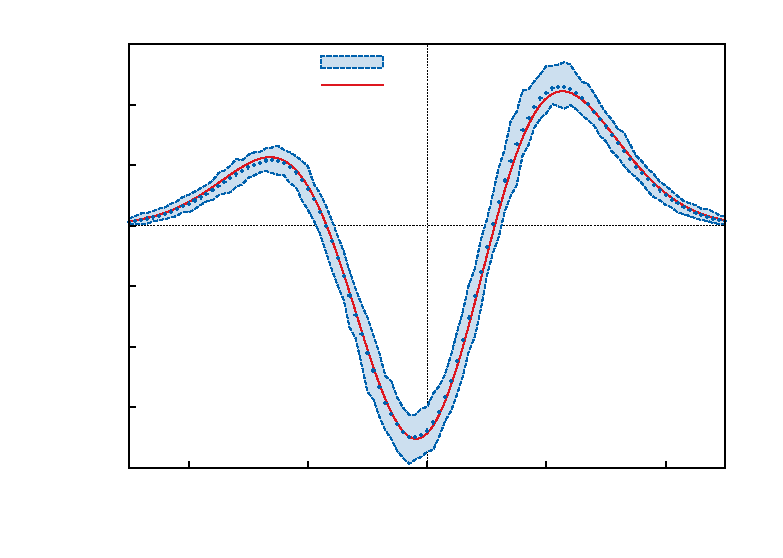
\includegraphics{./figures/elkc_exp_3D_gaussian_0}}%
    \gplfronttext
  \end{picture}%
\endgroup
}}\hspace{1.2cm}
  \subfigure{\scalebox{0.5}{% GNUPLOT: LaTeX picture with Postscript
\begingroup
  \makeatletter
  \providecommand\color[2][]{%
    \GenericError{(gnuplot) \space\space\space\@spaces}{%
      Package color not loaded in conjunction with
      terminal option `colourtext'%
    }{See the gnuplot documentation for explanation.%
    }{Either use 'blacktext' in gnuplot or load the package
      color.sty in LaTeX.}%
    \renewcommand\color[2][]{}%
  }%
  \providecommand\includegraphics[2][]{%
    \GenericError{(gnuplot) \space\space\space\@spaces}{%
      Package graphicx or graphics not loaded%
    }{See the gnuplot documentation for explanation.%
    }{The gnuplot epslatex terminal needs graphicx.sty or graphics.sty.}%
    \renewcommand\includegraphics[2][]{}%
  }%
  \providecommand\rotatebox[2]{#2}%
  \@ifundefined{ifGPcolor}{%
    \newif\ifGPcolor
    \GPcolorfalse
  }{}%
  \@ifundefined{ifGPblacktext}{%
    \newif\ifGPblacktext
    \GPblacktexttrue
  }{}%
  % define a \g@addto@macro without @ in the name:
  \let\gplgaddtomacro\g@addto@macro
  % define empty templates for all commands taking text:
  \gdef\gplbacktext{}%
  \gdef\gplfronttext{}%
  \makeatother
  \ifGPblacktext
    % no textcolor at all
    \def\colorrgb#1{}%
    \def\colorgray#1{}%
  \else
    % gray or color?
    \ifGPcolor
      \def\colorrgb#1{\color[rgb]{#1}}%
      \def\colorgray#1{\color[gray]{#1}}%
      \expandafter\def\csname LTw\endcsname{\color{white}}%
      \expandafter\def\csname LTb\endcsname{\color{black}}%
      \expandafter\def\csname LTa\endcsname{\color{black}}%
      \expandafter\def\csname LT0\endcsname{\color[rgb]{1,0,0}}%
      \expandafter\def\csname LT1\endcsname{\color[rgb]{0,1,0}}%
      \expandafter\def\csname LT2\endcsname{\color[rgb]{0,0,1}}%
      \expandafter\def\csname LT3\endcsname{\color[rgb]{1,0,1}}%
      \expandafter\def\csname LT4\endcsname{\color[rgb]{0,1,1}}%
      \expandafter\def\csname LT5\endcsname{\color[rgb]{1,1,0}}%
      \expandafter\def\csname LT6\endcsname{\color[rgb]{0,0,0}}%
      \expandafter\def\csname LT7\endcsname{\color[rgb]{1,0.3,0}}%
      \expandafter\def\csname LT8\endcsname{\color[rgb]{0.5,0.5,0.5}}%
    \else
      % gray
      \def\colorrgb#1{\color{black}}%
      \def\colorgray#1{\color[gray]{#1}}%
      \expandafter\def\csname LTw\endcsname{\color{white}}%
      \expandafter\def\csname LTb\endcsname{\color{black}}%
      \expandafter\def\csname LTa\endcsname{\color{black}}%
      \expandafter\def\csname LT0\endcsname{\color{black}}%
      \expandafter\def\csname LT1\endcsname{\color{black}}%
      \expandafter\def\csname LT2\endcsname{\color{black}}%
      \expandafter\def\csname LT3\endcsname{\color{black}}%
      \expandafter\def\csname LT4\endcsname{\color{black}}%
      \expandafter\def\csname LT5\endcsname{\color{black}}%
      \expandafter\def\csname LT6\endcsname{\color{black}}%
      \expandafter\def\csname LT7\endcsname{\color{black}}%
      \expandafter\def\csname LT8\endcsname{\color{black}}%
    \fi
  \fi
  \setlength{\unitlength}{0.0500bp}%
  \begin{picture}(7200.00,5040.00)%
    \gplgaddtomacro\gplbacktext{%
      \csname LTb\endcsname%
      \put(1078,704){\makebox(0,0)[r]{\strut{}-1000}}%
      \put(1078,1286){\makebox(0,0)[r]{\strut{}-500}}%
      \put(1078,1867){\makebox(0,0)[r]{\strut{} 0}}%
      \put(1078,2449){\makebox(0,0)[r]{\strut{} 500}}%
      \put(1078,3030){\makebox(0,0)[r]{\strut{} 1000}}%
      \put(1078,3612){\makebox(0,0)[r]{\strut{} 1500}}%
      \put(1078,4193){\makebox(0,0)[r]{\strut{} 2000}}%
      \put(1078,4775){\makebox(0,0)[r]{\strut{} 2500}}%
      \put(1769,484){\makebox(0,0){\strut{}-4}}%
      \put(2888,484){\makebox(0,0){\strut{}-2}}%
      \put(4007,484){\makebox(0,0){\strut{} 0}}%
      \put(5125,484){\makebox(0,0){\strut{} 2}}%
      \put(6244,484){\makebox(0,0){\strut{} 4}}%
      \csname LTb\endcsname%
      \put(176,2739){\rotatebox{90}{\makebox(0,0){\strut{}Half diameter}}}%
      \put(4006,154){\makebox(0,0){\strut{}$\lset$}}%
    }%
    \gplgaddtomacro\gplfronttext{%
      \csname LTb\endcsname%
      \put(5816,4602){\makebox(0,0)[r]{\strut{}Theoretical}}%
    }%
    \gplbacktext
    \put(0,0){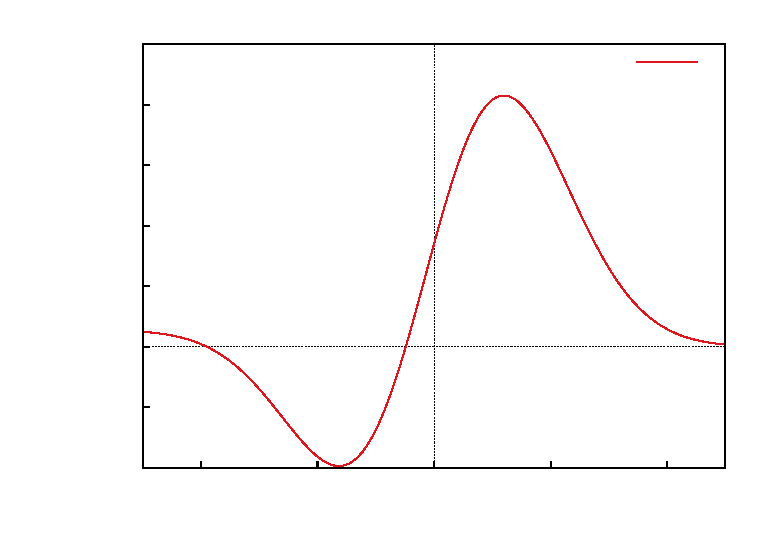
\includegraphics{./figures/elkc_exp_3D_gaussian_1}}%
    \gplfronttext
  \end{picture}%
\endgroup
}}\\
  \subfigure{\scalebox{0.5}{% GNUPLOT: LaTeX picture with Postscript
\begingroup
  \makeatletter
  \providecommand\color[2][]{%
    \GenericError{(gnuplot) \space\space\space\@spaces}{%
      Package color not loaded in conjunction with
      terminal option `colourtext'%
    }{See the gnuplot documentation for explanation.%
    }{Either use 'blacktext' in gnuplot or load the package
      color.sty in LaTeX.}%
    \renewcommand\color[2][]{}%
  }%
  \providecommand\includegraphics[2][]{%
    \GenericError{(gnuplot) \space\space\space\@spaces}{%
      Package graphicx or graphics not loaded%
    }{See the gnuplot documentation for explanation.%
    }{The gnuplot epslatex terminal needs graphicx.sty or graphics.sty.}%
    \renewcommand\includegraphics[2][]{}%
  }%
  \providecommand\rotatebox[2]{#2}%
  \@ifundefined{ifGPcolor}{%
    \newif\ifGPcolor
    \GPcolorfalse
  }{}%
  \@ifundefined{ifGPblacktext}{%
    \newif\ifGPblacktext
    \GPblacktexttrue
  }{}%
  % define a \g@addto@macro without @ in the name:
  \let\gplgaddtomacro\g@addto@macro
  % define empty templates for all commands taking text:
  \gdef\gplbacktext{}%
  \gdef\gplfronttext{}%
  \makeatother
  \ifGPblacktext
    % no textcolor at all
    \def\colorrgb#1{}%
    \def\colorgray#1{}%
  \else
    % gray or color?
    \ifGPcolor
      \def\colorrgb#1{\color[rgb]{#1}}%
      \def\colorgray#1{\color[gray]{#1}}%
      \expandafter\def\csname LTw\endcsname{\color{white}}%
      \expandafter\def\csname LTb\endcsname{\color{black}}%
      \expandafter\def\csname LTa\endcsname{\color{black}}%
      \expandafter\def\csname LT0\endcsname{\color[rgb]{1,0,0}}%
      \expandafter\def\csname LT1\endcsname{\color[rgb]{0,1,0}}%
      \expandafter\def\csname LT2\endcsname{\color[rgb]{0,0,1}}%
      \expandafter\def\csname LT3\endcsname{\color[rgb]{1,0,1}}%
      \expandafter\def\csname LT4\endcsname{\color[rgb]{0,1,1}}%
      \expandafter\def\csname LT5\endcsname{\color[rgb]{1,1,0}}%
      \expandafter\def\csname LT6\endcsname{\color[rgb]{0,0,0}}%
      \expandafter\def\csname LT7\endcsname{\color[rgb]{1,0.3,0}}%
      \expandafter\def\csname LT8\endcsname{\color[rgb]{0.5,0.5,0.5}}%
    \else
      % gray
      \def\colorrgb#1{\color{black}}%
      \def\colorgray#1{\color[gray]{#1}}%
      \expandafter\def\csname LTw\endcsname{\color{white}}%
      \expandafter\def\csname LTb\endcsname{\color{black}}%
      \expandafter\def\csname LTa\endcsname{\color{black}}%
      \expandafter\def\csname LT0\endcsname{\color{black}}%
      \expandafter\def\csname LT1\endcsname{\color{black}}%
      \expandafter\def\csname LT2\endcsname{\color{black}}%
      \expandafter\def\csname LT3\endcsname{\color{black}}%
      \expandafter\def\csname LT4\endcsname{\color{black}}%
      \expandafter\def\csname LT5\endcsname{\color{black}}%
      \expandafter\def\csname LT6\endcsname{\color{black}}%
      \expandafter\def\csname LT7\endcsname{\color{black}}%
      \expandafter\def\csname LT8\endcsname{\color{black}}%
    \fi
  \fi
  \setlength{\unitlength}{0.0500bp}%
  \begin{picture}(7200.00,5040.00)%
    \gplgaddtomacro\gplbacktext{%
      \csname LTb\endcsname%
      \put(1210,704){\makebox(0,0)[r]{\strut{} 0}}%
      \put(1210,1383){\makebox(0,0)[r]{\strut{} 2000}}%
      \put(1210,2061){\makebox(0,0)[r]{\strut{} 4000}}%
      \put(1210,2740){\makebox(0,0)[r]{\strut{} 6000}}%
      \put(1210,3418){\makebox(0,0)[r]{\strut{} 8000}}%
      \put(1210,4097){\makebox(0,0)[r]{\strut{} 10000}}%
      \put(1210,4775){\makebox(0,0)[r]{\strut{} 12000}}%
      \put(1888,484){\makebox(0,0){\strut{}-4}}%
      \put(2980,484){\makebox(0,0){\strut{}-2}}%
      \put(4073,484){\makebox(0,0){\strut{} 0}}%
      \put(5165,484){\makebox(0,0){\strut{} 2}}%
      \put(6257,484){\makebox(0,0){\strut{} 4}}%
      \csname LTb\endcsname%
      \put(176,2739){\rotatebox{90}{\makebox(0,0){\strut{}Surface area}}}%
      \put(4072,154){\makebox(0,0){\strut{}$\lset$}}%
    }%
    \gplgaddtomacro\gplfronttext{%
      \csname LTb\endcsname%
      \put(5816,4602){\makebox(0,0)[r]{\strut{}Theoretical}}%
    }%
    \gplbacktext
    \put(0,0){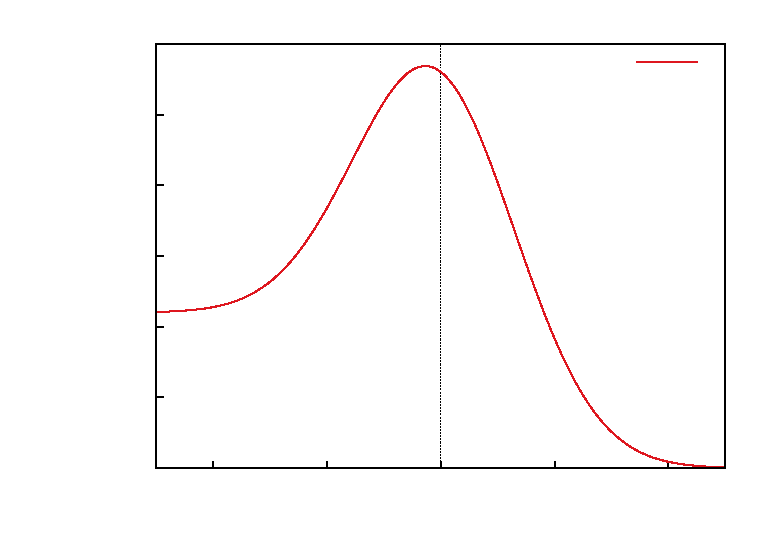
\includegraphics{./figures/elkc_exp_3D_gaussian_2}}%
    \gplfronttext
  \end{picture}%
\endgroup
}}\hspace{1.2cm}
  \subfigure{\scalebox{0.5}{% GNUPLOT: LaTeX picture with Postscript
\begingroup
  \makeatletter
  \providecommand\color[2][]{%
    \GenericError{(gnuplot) \space\space\space\@spaces}{%
      Package color not loaded in conjunction with
      terminal option `colourtext'%
    }{See the gnuplot documentation for explanation.%
    }{Either use 'blacktext' in gnuplot or load the package
      color.sty in LaTeX.}%
    \renewcommand\color[2][]{}%
  }%
  \providecommand\includegraphics[2][]{%
    \GenericError{(gnuplot) \space\space\space\@spaces}{%
      Package graphicx or graphics not loaded%
    }{See the gnuplot documentation for explanation.%
    }{The gnuplot epslatex terminal needs graphicx.sty or graphics.sty.}%
    \renewcommand\includegraphics[2][]{}%
  }%
  \providecommand\rotatebox[2]{#2}%
  \@ifundefined{ifGPcolor}{%
    \newif\ifGPcolor
    \GPcolorfalse
  }{}%
  \@ifundefined{ifGPblacktext}{%
    \newif\ifGPblacktext
    \GPblacktexttrue
  }{}%
  % define a \g@addto@macro without @ in the name:
  \let\gplgaddtomacro\g@addto@macro
  % define empty templates for all commands taking text:
  \gdef\gplbacktext{}%
  \gdef\gplfronttext{}%
  \makeatother
  \ifGPblacktext
    % no textcolor at all
    \def\colorrgb#1{}%
    \def\colorgray#1{}%
  \else
    % gray or color?
    \ifGPcolor
      \def\colorrgb#1{\color[rgb]{#1}}%
      \def\colorgray#1{\color[gray]{#1}}%
      \expandafter\def\csname LTw\endcsname{\color{white}}%
      \expandafter\def\csname LTb\endcsname{\color{black}}%
      \expandafter\def\csname LTa\endcsname{\color{black}}%
      \expandafter\def\csname LT0\endcsname{\color[rgb]{1,0,0}}%
      \expandafter\def\csname LT1\endcsname{\color[rgb]{0,1,0}}%
      \expandafter\def\csname LT2\endcsname{\color[rgb]{0,0,1}}%
      \expandafter\def\csname LT3\endcsname{\color[rgb]{1,0,1}}%
      \expandafter\def\csname LT4\endcsname{\color[rgb]{0,1,1}}%
      \expandafter\def\csname LT5\endcsname{\color[rgb]{1,1,0}}%
      \expandafter\def\csname LT6\endcsname{\color[rgb]{0,0,0}}%
      \expandafter\def\csname LT7\endcsname{\color[rgb]{1,0.3,0}}%
      \expandafter\def\csname LT8\endcsname{\color[rgb]{0.5,0.5,0.5}}%
    \else
      % gray
      \def\colorrgb#1{\color{black}}%
      \def\colorgray#1{\color[gray]{#1}}%
      \expandafter\def\csname LTw\endcsname{\color{white}}%
      \expandafter\def\csname LTb\endcsname{\color{black}}%
      \expandafter\def\csname LTa\endcsname{\color{black}}%
      \expandafter\def\csname LT0\endcsname{\color{black}}%
      \expandafter\def\csname LT1\endcsname{\color{black}}%
      \expandafter\def\csname LT2\endcsname{\color{black}}%
      \expandafter\def\csname LT3\endcsname{\color{black}}%
      \expandafter\def\csname LT4\endcsname{\color{black}}%
      \expandafter\def\csname LT5\endcsname{\color{black}}%
      \expandafter\def\csname LT6\endcsname{\color{black}}%
      \expandafter\def\csname LT7\endcsname{\color{black}}%
      \expandafter\def\csname LT8\endcsname{\color{black}}%
    \fi
  \fi
  \setlength{\unitlength}{0.0500bp}%
  \begin{picture}(7200.00,5040.00)%
    \gplgaddtomacro\gplbacktext{%
      \csname LTb\endcsname%
      \put(1210,704){\makebox(0,0)[r]{\strut{} 0}}%
      \put(1210,1213){\makebox(0,0)[r]{\strut{} 5000}}%
      \put(1210,1722){\makebox(0,0)[r]{\strut{} 10000}}%
      \put(1210,2231){\makebox(0,0)[r]{\strut{} 15000}}%
      \put(1210,2740){\makebox(0,0)[r]{\strut{} 20000}}%
      \put(1210,3248){\makebox(0,0)[r]{\strut{} 25000}}%
      \put(1210,3757){\makebox(0,0)[r]{\strut{} 30000}}%
      \put(1210,4266){\makebox(0,0)[r]{\strut{} 35000}}%
      \put(1210,4775){\makebox(0,0)[r]{\strut{} 40000}}%
      \put(1888,484){\makebox(0,0){\strut{}-4}}%
      \put(2980,484){\makebox(0,0){\strut{}-2}}%
      \put(4073,484){\makebox(0,0){\strut{} 0}}%
      \put(5165,484){\makebox(0,0){\strut{} 2}}%
      \put(6257,484){\makebox(0,0){\strut{} 4}}%
      \csname LTb\endcsname%
      \put(176,2739){\rotatebox{90}{\makebox(0,0){\strut{}Volume}}}%
      \put(4072,154){\makebox(0,0){\strut{}$\lset$}}%
    }%
    \gplgaddtomacro\gplfronttext{%
      \csname LTb\endcsname%
      \put(5816,4602){\makebox(0,0)[r]{\strut{}Experimental}}%
      \csname LTb\endcsname%
      \put(5816,4382){\makebox(0,0)[r]{\strut{}Theoretical}}%
    }%
    \gplbacktext
    \put(0,0){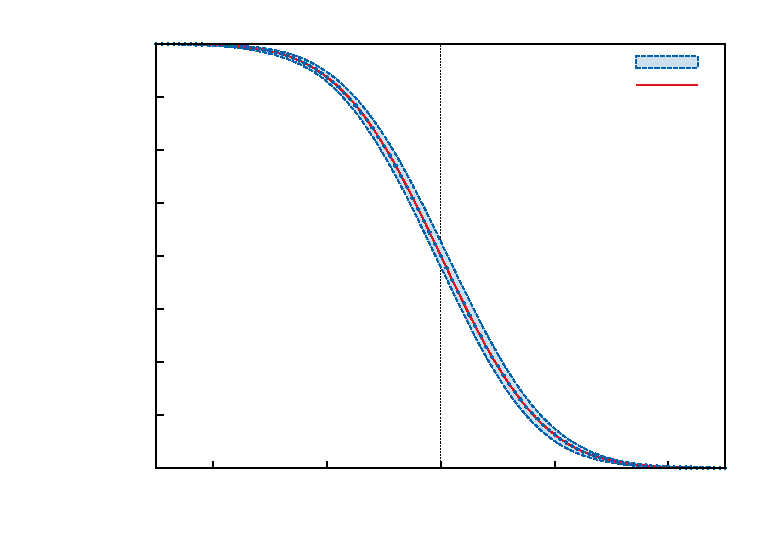
\includegraphics{./figures/elkc_exp_3D_gaussian_3}}%
    \gplfronttext
  \end{picture}%
\endgroup
}}\\
  \caption{Expectation of LKC for $\PRF=100\times 20 \times 20$, $\mean=0.0$, $\std^2=2$, $\Lc=2$, and $\HS=\uinf$ (gaussian distribution with tail hitting set) in 3D. Experimental results are calculated over $100$ realizations.}
\end{figure}

\newpage
\section{Size effect}
In this section another approach using expected values of excursion set characteristics is proposed. Up to this point, this mathematical tool has been used in order to yield actual morphologies and predict their geometrical and topological characteristics. The continuum aspect of correlated RFs was concealed by the thresholding method used (level set) which led to discrete fields (excursion sets). Herein, RFs directly represent a material property (ultimate stress field) and the excursion set theory is used in order to catch statistical information on its extrema.
\par A theoretical method for size effect modeling of brittle heterogeneous materials is proposed. In this field, the main result comes from the early studies of \cite{weibull_statistical_1951} based on the theory of the weakest link. The authors proposed an analytical solution for the global failure criterion, considering a discrete structure of independent brittle links with a specific distribution probability of local failure criterion. With no spatial correlation between each link, this theory leads inevitably to large scale size effect. The two current theories of Zden\v{e}k P. Ba\v{z}ant and Alberto Carpinteri, trying to describe the size effect for the missing scales, are the main results of the extensive literature existing on this topic. The former tends, in many ways, to describe the size effect using both non-local model and stochastic approach \cite{sab_unified_1993}, or more recently using the so-called energetic-statistical size effect mixing strength redistribution theory in a fracture process zone and Weibull's theory \cite{bazant_probability_2004}. The latter considers material heterogeneities with a fractal model in order to represent size effects for quasi-brittle materials \cite{carpinteri_mechanics_2003}. On the other hand, numerical simulations have been made using stochastic integrations and correlated RFs in order to describe material properties \cite{colliat_stochastic_2007}. These methods are quickly time consuming and the underlying numerical implementation brings an inevitable limitation regarding the observation scale.
\par The idea behind this method is to extend the Weibull theory to lower scales by adding the spatial structure of \emph{correlated} RFs. A continuum representation of the spatial variability through scales can theoretically be made by defining a ratio $\rl=\Lc/\Msize$ between the spatial parameter of the correlated RF covariance function $\Lc$ and the size of its definition domaine $\Msize$. As already stated just above, heterogeneities modeling is directly made through a variation of material properties (and not by through definition of different phases). The continuum aspect of correlated RFs statistically represents a local ultimate failure stress $\slim(\x,\w)$ on a structure $\MRF$. RFs are here used in a direct way, even if the discrete aspect of excursion set and their expected Euler characteristic are used in order to define the global failure stress $\sfail$ of the structure. The whole framework has to be seen on a purely theoretical and analytical point of view. Contrary to stochastic integration methods, the knowledge of expected information on RFs avoids generating actual RF realizations. Hence, there is no scale limitation.

\subsection{Correlation lengths as scale parameters}
As it has been pointed out during this chapter, the correlation length $\Lc$ can been seen as a size parameter of a correlated RF. Herein, a constant value of $\Lc$ is chosen, fixing the average size of the heterogeneities considered. The dimension of the domain $\MRF$ (where the RF is defined) represents the size of the whole structure. If $\Msize$ is the characteristic length of $\MRF$ (for example: the length of a segment in the one-dimensional space, the length of the side of a square in a two-dimensional space\dots), its value determines the observation scale. In order to let the heterogeneity size unspecified, the ratio $\rl=\Lc/\Msize$ is taken into consideration. Nonetheless, $\Lc$ still as to be seen as a constant and $\Msize$ a variable. Realizations of RFs for different ratios $\rl$ are shown in Fig. \ref{fig:size-efect:rf2d} on a two-dimensional square.
\begin{description}
  \item \emph{For $\rl \gg 1$} \\ The structure is very small compared to the heterogeneity size. The RF tends to be a constant field and is equivalent to a single RV with no spatial information. It represents the material scale, the validity domain of continuum damage mechanics (CDM) where the failure stress does not depend on the size of the structure (see Fig. \ref{fig:size-efect:rf2d:1}).
  \item \emph{For $\rl \ll 1$} \\ The structure is very large compared to the heterogeneity size. The RF tends to be equivalent to a white noise (completely uncorrelated), leading to a loss of spatial structures. It represents the scale of big structures as the Weibull theory does, retrieving the linear fracture mechanic (LFM) domain of expertise (see Fig. \ref{fig:size-efect:rf2d:3}).
  \item \emph{For $\rl \approx 1$} \\ The RF represents the missing scale range where the continuum statistical information of correlated RFs for various $\rl$ can link together material and big structure scales. Hence, it can model size effect for civil engineering structures (see Fig. \ref{fig:size-efect:rf2d:2}).
\end{description}
\begin{figure}[h!]
  \centering\hspace*{\fill}
  \subfigure[$\rl \gg 1$.\label{fig:size-efect:rf2d:1}]{\epsfig{figure=./figures/fromPhD/Lc_big.eps,width=0.3\linewidth}}\hfill
  \subfigure[$\rl \approx 1$.\label{fig:size-efect:rf2d:2}]{\epsfig{figure=./figures/fromPhD/Lc_small.eps,width=0.3\linewidth}}\hfill
  \subfigure[$\rl \ll 1$.\label{fig:size-efect:rf2d:3}]{\epsfig{figure=./figures/fromPhD/Lc_white_noise.eps,width=0.3\linewidth}}\hspace*{\fill}
  \caption{Realization of two-dimensional correlated RFs for various $\rl$ ratios.\label{fig:size-efect:rf2d}}
\end{figure}

\subsection{One dimensional case}
In this study, a one-dimensional bar in tension is considered. The source of uncertainty is modeled by a statistical representation of the local failure criterion $\slim(x,\w)$. Due to the positiveness of stress fields in tension, the \emph{log-normal} distribution is used. Since log-normal distribution is Gaussian related, the results of the previous section are applicable by a simple transformation of the hitting set $S=\exp$. The spatial structure representation is done by using correlated RF with Gaussian covariance function of correlation length $\Lc$. The continuum domain represented is a one-dimensional bar $\MRF$ of length $\Msize$. For this specific case, the global brittle failure of a bar $\MRF$ is assumed to occur when, at least, the minimum value of $\slim(x,\w)$ is reached by the stress field. If $\sfail(\w)$ is this criterion, it can be defined for a realization $i$ by: 
\begin{equation}
  \sfail(\w_i) = \underset{x \in \MRF_i}{\inf}\left(\slim(x,\w_i)\right).
  \label{eq:size-effect:failure-criterion}
\end{equation}
It occurs that this equation can directly be linked with the Euler characteristic $\EC$ of an excursion sets. Let $\ES(\s) = \left\{x \in \MRF \ | \ 0 \le \sigma_{y}(x,\omega)\leq\s \ \right\}$ be an excursion set where the constant stress state of the bar can been seen as a level set. With this definition, the excursion set represents the part of the bar (subset of $\MRF$) where the stress is above the local failure criterion $\slim(x,\w)$. The global failure criterion of Eq. \ref{eq:size-effect:failure-criterion} can therefore be seen in terms of excursion set; $\sfail$ being the stress state when, with increasing $\s$, $\ES(\s)$ changes from being a void subset of $\MRF$ ($\EC = 0$) to a single connected component ($\EC = 1$).
\par A result of \cite{adler_new_2008} on statistical thresholding technics links the probability of reaching these minima and the expected Euler characteristic as follows:
\begin{equation}
  \label{eq:size-effect:prob-failure-criterion}
  \Proba\left\{ \underset{x\in \MRF}{\inf}\left( \slim(x,\w) \right) \leq \s \right\} \approx \Expec\left\{ \EC\left(\ES(\s)\right) \right\} \ \ \text{``for low $\sigma$''}.
\end{equation}
The major improvement that Eq. \ref{eq:size-effect:prob-failure-criterion} provides is the knowledge of statistical information on $\sfail(\w)$, and with it, the need of Monte Carlo simulations with actual realizations $i$ as suggested by Eq. \ref{eq:size-effect:failure-criterion}. Then, the initial failure criterion of the structure can be reformulated in terms of probability $q$. This leads to:
\begin{equation}
	\label{eq:size-effect:global-stress}
	\sfail(q) = \left\{ \s \ | \ \Proba\left\{ \underset{x\in \MRF}{\inf}\left( \slim(x,\w) \right) \leq \s \right\} = q \right\}.
\end{equation}
The expected value of the Euler characteristic being analytically known, Eq. \ref{eq:size-effect:prob-failure-criterion} and Eq. \ref{eq:size-effect:global-stress} allow the ultimate stress criterion of the bar to be analytically determined, for a given failure probability $q$.
\par In order to scan every observation scales possible, Eq. \ref{eq:size-effect:global-stress} is solved for a large scale range $10^{-9}\le\rl\le10^3$. Since $\Lc$ is fixed by the heterogeneity size, the different scales are therefore represented by defining a single $\slim(x,\w)$ (with the same covariance function) for various $\Msize$ as represented in Fig. \ref{fig:size-effect:1D-various-sizes}. The mean and the variance of the log-normal correlated RF have physical meaning and can be determined depending on the material characteristics. While the mean value of $\slim(x,\omega)$ determines the value of the structural failure stress of small scales ($\rl\gg1$), its variance indicates the decreasing rate of the size effect for large scales ($\rl\ll1$).
\begin{figure}[h!]
  \centering
  \scalebox{0.55}{\LARGE% Generated with LaTeXDraw 2.0.8
% Thu Jun 20 13:43:41 CEST 2013
% \usepackage[usenames,dvipsnames]{pstricks}
% \usepackage{epsfig}
% \usepackage{pst-grad} % For gradients
% \usepackage{pst-plot} % For axes
\scalebox{1} % Change this value to rescale the drawing.
{
\begin{pspicture}(0,-4.71)(16.64,4.71)
\psline[linewidth=0.08cm,tbarsize=0.07055555cm 5.0]{|*-|*}(2.2,1.21)(5.8,1.21)
\psline[linewidth=0.08cm,tbarsize=0.07055555cm 5.0]{|*-|*}(7.0,1.21)(16.6,1.21)
\psline[linewidth=0.08cm,tbarsize=0.07055555cm 5.0]{|*-|*}(2.2,-3.59)(16.6,-3.59)
\psbezier[linewidth=0.04](2.2,2.41)(3.0,4.01)(3.2,4.41)(3.4,3.01)(3.6,1.61)(4.2,1.41)(4.6,2.41)(5.0,3.41)(5.2,4.21)(5.8,2.41)
\psbezier[linewidth=0.04](7.0,2.41)(7.8,1.01)(8.0,2.01)(8.2,2.81)(8.4,3.61)(8.8,4.01)(9.4,2.41)(10.0,0.81)(10.2,2.81)(10.6,3.01)(11.0,3.21)(10.8,1.81)(11.8,1.81)(12.8,1.81)(12.2,4.01)(13.0,3.61)(13.8,3.21)(13.8,1.61)(14.2,2.41)(14.6,3.21)(14.6,2.01)(15.6,1.81)(16.6,1.61)(16.0,4.21)(16.6,3.21)
\psbezier[linewidth=0.04](2.2,-2.39)(2.8,-2.99)(2.4,-3.19)(3.4,-3.19)(4.4,-3.19)(3.6,-0.59)(4.6,-1.19)(5.6,-1.79)(5.4,-4.19)(5.8,-2.19)(6.2,-0.19)(6.4,-4.19)(7.0,-2.99)(7.6,-1.79)(7.6,-0.19)(8.2,-1.39)(8.8,-2.59)(9.2,-3.79)(9.4,-2.99)(9.6,-2.19)(9.6,-1.59)(10.6,-1.59)(11.6,-1.59)(11.0,-3.39)(11.8,-2.39)(12.6,-1.39)(12.4,-2.79)(13.0,-1.39)(13.6,0.01)(13.2,-2.39)(14.2,-2.39)(15.2,-2.39)(14.4,-3.39)(15.4,-3.39)(16.4,-3.39)(15.8,0.01)(16.6,-2.39)
\usefont{T1}{ptm}{m}{n}
\rput(4.05,0.315){$\Msize_1$}
\usefont{T1}{ptm}{m}{n}
\rput(11.85,0.315){$\Msize_2$}
\usefont{T1}{ptm}{m}{n}
\rput(8.85,-4.485){$\Msize_3$}
\psline[linewidth=0.04cm,arrowsize=0.05291667cm 2.0,arrowlength=1.4,arrowinset=0.4]{<->}(3.0,4.01)(4.2,4.01)
\usefont{T1}{ptm}{m}{n}
\rput(3.62,4.515){$\Lc$}
\psline[linewidth=0.04cm,arrowsize=0.05291667cm 2.0,arrowlength=1.4,arrowinset=0.4]{<->}(8.6,3.81)(9.8,3.81)
\usefont{T1}{ptm}{m}{n}
\rput(9.22,4.315){$\Lc$}
\psline[linewidth=0.04cm,arrowsize=0.05291667cm 2.0,arrowlength=1.4,arrowinset=0.4]{<->}(7.8,-0.79)(9.0,-0.79)
\usefont{T1}{ptm}{m}{n}
\rput(8.42,-0.285){$\Lc$}
\psline[linewidth=0.04cm,tbarsize=0.07055555cm 5.0,arrowsize=0.05291667cm 2.0,arrowlength=1.4,arrowinset=0.4]{|*->}(1.0,1.21)(1.0,4.41)
\usefont{T1}{ptm}{m}{n}
\rput(0.54,4.115){$\slim$}
\psline[linewidth=0.04cm,tbarsize=0.07055555cm 5.0,arrowsize=0.05291667cm 2.0,arrowlength=1.4,arrowinset=0.4]{|*->}(1.0,-3.59)(1.0,-0.39)
\usefont{T1}{ptm}{m}{n}
\rput(0.54,-0.685){$\slim$}
\end{pspicture} 
}
}
  \caption{Illustration of the local failure stress repartition on structures of various sizes.\label{fig:size-effect:1D-various-sizes}}
\end{figure}
\par In order to validate the theoretical framework, results of the same problem solved using a Monte-Carlo stochastic integration method are also given. On the one hand, the stochastic integration provides a full empirical distribution of $\sfail(\w)$ (defined by Eq. \ref{eq:size-effect:failure-criterion}) for several ratios $\rl$. On the other hand, the analytical results of $\sfail(q)$ depends directly on the probability parameter $q$ that, by definition of the ultimate stress Eq. \ref{eq:size-effect:global-stress}, is directly linked with quantiles of the previous empirical distribution. For example, $q=1/2$ corresponds to the $2$-quantile, \ie the median.
\par Fig. \ref{graph:size-effect:results:p} shows the resulting global failure stresses $\sfail$ for ratio $\rlinv=\rl^{-1}$ from $10^{-3}$ to $10^2$ with the Monte-Carlo method (in order to show results in the most commonly used manner, scales are represented by the inverse ratio $\rlinv=\rl^{-1}=\Msize/\Lc$). The inspection of larger scales is rapidly limited by the inconvenient resource consuming aspect of stochastic integrations. On the strength of its analytical base, the excursion set theory every scale can be inspected, here for $\rlinv$ varying from $10^{-3}$ to $10^{9}$. The Monte-Carlo integration results of global the failure stress distribution is given for the $2$, $10$, and $100$-quantile, corresponding to $q=1/2$, $1/10$, and $1/100$, respectively. In both method, the mean and the variance of the \emph{log-normal} distribution are both taken to be $10$. The \textsc{RandomFields} package \cite{schlather_randomfields:_2012} of the \textsc{R} environment \cite{team_r:_2012} has been used in order to do the stochastic integration, using $10\,000$ integration points for each length. 
\begin{figure}[h!]
  \centering\hspace*{\fill}
  \subfigure[Comparison between theoretical results and Monte-Carlo simulations for various quantiles.\label{graph:size-effect:results:p}]{\scalebox{0.55}{% GNUPLOT: LaTeX picture with Postscript
\begingroup
  \makeatletter
  \providecommand\color[2][]{%
    \GenericError{(gnuplot) \space\space\space\@spaces}{%
      Package color not loaded in conjunction with
      terminal option `colourtext'%
    }{See the gnuplot documentation for explanation.%
    }{Either use 'blacktext' in gnuplot or load the package
      color.sty in LaTeX.}%
    \renewcommand\color[2][]{}%
  }%
  \providecommand\includegraphics[2][]{%
    \GenericError{(gnuplot) \space\space\space\@spaces}{%
      Package graphicx or graphics not loaded%
    }{See the gnuplot documentation for explanation.%
    }{The gnuplot epslatex terminal needs graphicx.sty or graphics.sty.}%
    \renewcommand\includegraphics[2][]{}%
  }%
  \providecommand\rotatebox[2]{#2}%
  \@ifundefined{ifGPcolor}{%
    \newif\ifGPcolor
    \GPcolorfalse
  }{}%
  \@ifundefined{ifGPblacktext}{%
    \newif\ifGPblacktext
    \GPblacktexttrue
  }{}%
  % define a \g@addto@macro without @ in the name:
  \let\gplgaddtomacro\g@addto@macro
  % define empty templates for all commands taking text:
  \gdef\gplbacktext{}%
  \gdef\gplfronttext{}%
  \makeatother
  \ifGPblacktext
    % no textcolor at all
    \def\colorrgb#1{}%
    \def\colorgray#1{}%
  \else
    % gray or color?
    \ifGPcolor
      \def\colorrgb#1{\color[rgb]{#1}}%
      \def\colorgray#1{\color[gray]{#1}}%
      \expandafter\def\csname LTw\endcsname{\color{white}}%
      \expandafter\def\csname LTb\endcsname{\color{black}}%
      \expandafter\def\csname LTa\endcsname{\color{black}}%
      \expandafter\def\csname LT0\endcsname{\color[rgb]{1,0,0}}%
      \expandafter\def\csname LT1\endcsname{\color[rgb]{0,1,0}}%
      \expandafter\def\csname LT2\endcsname{\color[rgb]{0,0,1}}%
      \expandafter\def\csname LT3\endcsname{\color[rgb]{1,0,1}}%
      \expandafter\def\csname LT4\endcsname{\color[rgb]{0,1,1}}%
      \expandafter\def\csname LT5\endcsname{\color[rgb]{1,1,0}}%
      \expandafter\def\csname LT6\endcsname{\color[rgb]{0,0,0}}%
      \expandafter\def\csname LT7\endcsname{\color[rgb]{1,0.3,0}}%
      \expandafter\def\csname LT8\endcsname{\color[rgb]{0.5,0.5,0.5}}%
    \else
      % gray
      \def\colorrgb#1{\color{black}}%
      \def\colorgray#1{\color[gray]{#1}}%
      \expandafter\def\csname LTw\endcsname{\color{white}}%
      \expandafter\def\csname LTb\endcsname{\color{black}}%
      \expandafter\def\csname LTa\endcsname{\color{black}}%
      \expandafter\def\csname LT0\endcsname{\color{black}}%
      \expandafter\def\csname LT1\endcsname{\color{black}}%
      \expandafter\def\csname LT2\endcsname{\color{black}}%
      \expandafter\def\csname LT3\endcsname{\color{black}}%
      \expandafter\def\csname LT4\endcsname{\color{black}}%
      \expandafter\def\csname LT5\endcsname{\color{black}}%
      \expandafter\def\csname LT6\endcsname{\color{black}}%
      \expandafter\def\csname LT7\endcsname{\color{black}}%
      \expandafter\def\csname LT8\endcsname{\color{black}}%
    \fi
  \fi
  \setlength{\unitlength}{0.0500bp}%
  \begin{picture}(7200.00,5040.00)%
    \gplgaddtomacro\gplbacktext{%
      \csname LTb\endcsname%
      \put(946,704){\makebox(0,0)[r]{\strut{} 0.1}}%
      \put(946,4775){\makebox(0,0)[r]{\strut{} 1}}%
      \put(1555,484){\makebox(0,0){\strut{}1e-2}}%
      \put(2509,484){\makebox(0,0){\strut{}1e0}}%
      \put(3463,484){\makebox(0,0){\strut{}1e2}}%
      \put(4418,484){\makebox(0,0){\strut{}1e4}}%
      \put(5372,484){\makebox(0,0){\strut{}1e6}}%
      \put(6326,484){\makebox(0,0){\strut{}1e8}}%
      \put(176,2739){\rotatebox{-270}{\makebox(0,0){\strut{}Normalized failure stress}}}%
      \put(3940,154){\makebox(0,0){\strut{}Scale ratio $\rlinv = \rl^{-1}$}}%
    }%
    \gplgaddtomacro\gplfronttext{%
      \csname LTb\endcsname%
      \put(2266,1317){\makebox(0,0)[r]{\strut{}$q = 0.5$}}%
      \csname LTb\endcsname%
      \put(2266,1097){\makebox(0,0)[r]{\strut{}$q = 0.1$}}%
      \csname LTb\endcsname%
      \put(2266,877){\makebox(0,0)[r]{\strut{}$q = 0.01$}}%
    }%
    \gplbacktext
    \put(0,0){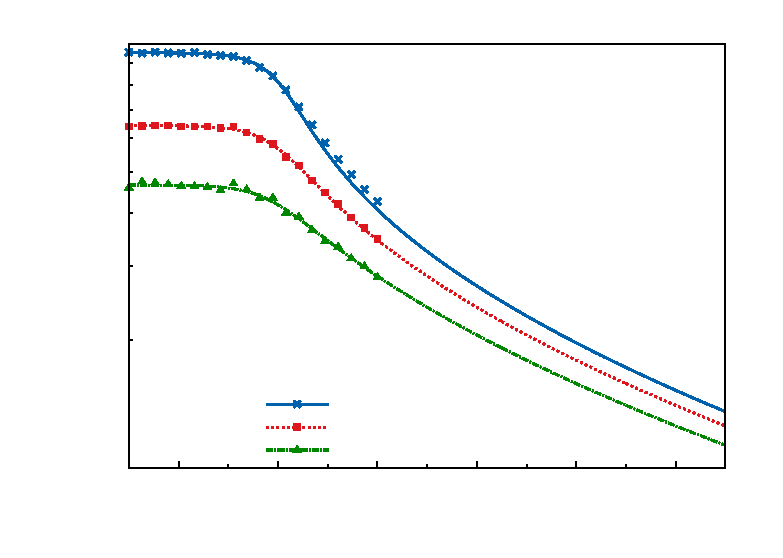
\includegraphics{./figures/fromPhD/log_1D_MonteCarlo_p}}%
    \gplfronttext
  \end{picture}%
\endgroup
}}\hfill
  \subfigure[Impact of the variance on the size effect.\label{graph:size-effect:results:v}]{\scalebox{0.55}{% GNUPLOT: LaTeX picture with Postscript
\begingroup
  \makeatletter
  \providecommand\color[2][]{%
    \GenericError{(gnuplot) \space\space\space\@spaces}{%
      Package color not loaded in conjunction with
      terminal option `colourtext'%
    }{See the gnuplot documentation for explanation.%
    }{Either use 'blacktext' in gnuplot or load the package
      color.sty in LaTeX.}%
    \renewcommand\color[2][]{}%
  }%
  \providecommand\includegraphics[2][]{%
    \GenericError{(gnuplot) \space\space\space\@spaces}{%
      Package graphicx or graphics not loaded%
    }{See the gnuplot documentation for explanation.%
    }{The gnuplot epslatex terminal needs graphicx.sty or graphics.sty.}%
    \renewcommand\includegraphics[2][]{}%
  }%
  \providecommand\rotatebox[2]{#2}%
  \@ifundefined{ifGPcolor}{%
    \newif\ifGPcolor
    \GPcolorfalse
  }{}%
  \@ifundefined{ifGPblacktext}{%
    \newif\ifGPblacktext
    \GPblacktexttrue
  }{}%
  % define a \g@addto@macro without @ in the name:
  \let\gplgaddtomacro\g@addto@macro
  % define empty templates for all commands taking text:
  \gdef\gplbacktext{}%
  \gdef\gplfronttext{}%
  \makeatother
  \ifGPblacktext
    % no textcolor at all
    \def\colorrgb#1{}%
    \def\colorgray#1{}%
  \else
    % gray or color?
    \ifGPcolor
      \def\colorrgb#1{\color[rgb]{#1}}%
      \def\colorgray#1{\color[gray]{#1}}%
      \expandafter\def\csname LTw\endcsname{\color{white}}%
      \expandafter\def\csname LTb\endcsname{\color{black}}%
      \expandafter\def\csname LTa\endcsname{\color{black}}%
      \expandafter\def\csname LT0\endcsname{\color[rgb]{1,0,0}}%
      \expandafter\def\csname LT1\endcsname{\color[rgb]{0,1,0}}%
      \expandafter\def\csname LT2\endcsname{\color[rgb]{0,0,1}}%
      \expandafter\def\csname LT3\endcsname{\color[rgb]{1,0,1}}%
      \expandafter\def\csname LT4\endcsname{\color[rgb]{0,1,1}}%
      \expandafter\def\csname LT5\endcsname{\color[rgb]{1,1,0}}%
      \expandafter\def\csname LT6\endcsname{\color[rgb]{0,0,0}}%
      \expandafter\def\csname LT7\endcsname{\color[rgb]{1,0.3,0}}%
      \expandafter\def\csname LT8\endcsname{\color[rgb]{0.5,0.5,0.5}}%
    \else
      % gray
      \def\colorrgb#1{\color{black}}%
      \def\colorgray#1{\color[gray]{#1}}%
      \expandafter\def\csname LTw\endcsname{\color{white}}%
      \expandafter\def\csname LTb\endcsname{\color{black}}%
      \expandafter\def\csname LTa\endcsname{\color{black}}%
      \expandafter\def\csname LT0\endcsname{\color{black}}%
      \expandafter\def\csname LT1\endcsname{\color{black}}%
      \expandafter\def\csname LT2\endcsname{\color{black}}%
      \expandafter\def\csname LT3\endcsname{\color{black}}%
      \expandafter\def\csname LT4\endcsname{\color{black}}%
      \expandafter\def\csname LT5\endcsname{\color{black}}%
      \expandafter\def\csname LT6\endcsname{\color{black}}%
      \expandafter\def\csname LT7\endcsname{\color{black}}%
      \expandafter\def\csname LT8\endcsname{\color{black}}%
    \fi
  \fi
  \setlength{\unitlength}{0.0500bp}%
  \begin{picture}(7200.00,5040.00)%
    \gplgaddtomacro\gplbacktext{%
      \csname LTb\endcsname%
      \put(946,704){\makebox(0,0)[r]{\strut{} 0.1}}%
      \put(946,4775){\makebox(0,0)[r]{\strut{} 1}}%
      \put(1555,484){\makebox(0,0){\strut{}1e-2}}%
      \put(2509,484){\makebox(0,0){\strut{}1e0}}%
      \put(3463,484){\makebox(0,0){\strut{}1e2}}%
      \put(4418,484){\makebox(0,0){\strut{}1e4}}%
      \put(5372,484){\makebox(0,0){\strut{}1e6}}%
      \put(6326,484){\makebox(0,0){\strut{}1e8}}%
      \put(176,2739){\rotatebox{-270}{\makebox(0,0){\strut{}Normalized failure stress}}}%
      \put(3940,154){\makebox(0,0){\strut{}Scale ratio $\rlinv = \rl^{-1}$}}%
    }%
    \gplgaddtomacro\gplfronttext{%
      \csname LTb\endcsname%
      \put(2662,1317){\makebox(0,0)[r]{\strut{}variance $1$}}%
      \csname LTb\endcsname%
      \put(2662,1097){\makebox(0,0)[r]{\strut{}variance $5$}}%
      \csname LTb\endcsname%
      \put(2662,877){\makebox(0,0)[r]{\strut{}variance $10$}}%
    }%
    \gplbacktext
    \put(0,0){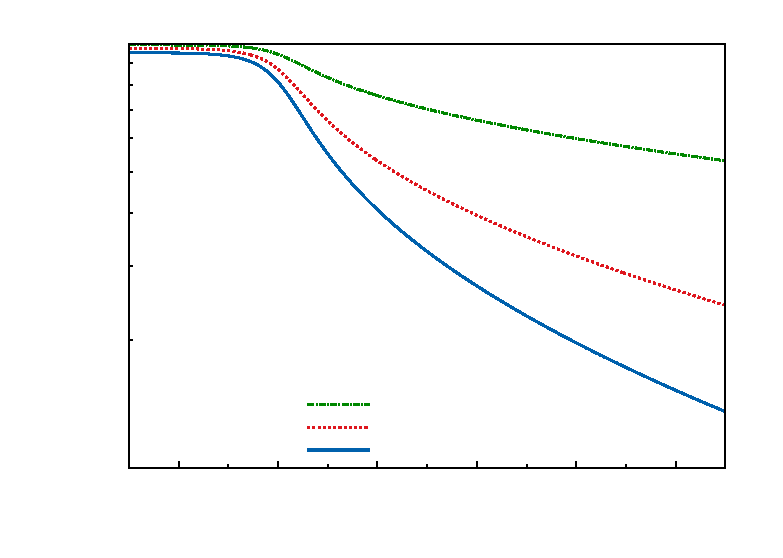
\includegraphics{./figures/fromPhD/log_1D_var_v}}%
    \gplfronttext
  \end{picture}%
\endgroup
}}\hspace*{\fill}
  \caption{Representation of the size effect through a failure stress criterion estimated for various scales.\label{graph:size-effect:results}}
\end{figure}
\par As expected, no size effect is observed at the small scale, $\rlinv < 10^{-2}$. For $q=1/2$, the value of the failure stress corresponds to the \emph{log-normal} distribution median (that is, due to the skewness of the distribution, a little less than the mean). As $\rlinv$ grows, the decrease of $\sfail$ representing the size effect can be seen. As for the impact of $q$, results show the good behavior. Indeed, for a safety probability of $90\%$ (meaning a failure probability of $q=0.1$), the failure stress is higher than for a safety of $99\%$ ($q=0.01$). The three curves drawn in Fig. \ref{graph:size-effect:results:v} represent the impact of the variance on size effect for a failure probability $q=1/2$. While $\Lc$ is the parameter of the correlated RF that represents the geometry of the heterogeneities, the variance can be seen as a description of the mechanical property discrepancy. Results show the natural principle that higher variations are, lower the values and larger the drop of $\sfail$ are.
\begin{figure}[!h]
  \centering
    \hspace*{\fill}
  \subfigure[Variation of the quantile]{\scalebox{0.5}{% GNUPLOT: LaTeX picture with Postscript
\begingroup
  \makeatletter
  \providecommand\color[2][]{%
    \GenericError{(gnuplot) \space\space\space\@spaces}{%
      Package color not loaded in conjunction with
      terminal option `colourtext'%
    }{See the gnuplot documentation for explanation.%
    }{Either use 'blacktext' in gnuplot or load the package
      color.sty in LaTeX.}%
    \renewcommand\color[2][]{}%
  }%
  \providecommand\includegraphics[2][]{%
    \GenericError{(gnuplot) \space\space\space\@spaces}{%
      Package graphicx or graphics not loaded%
    }{See the gnuplot documentation for explanation.%
    }{The gnuplot epslatex terminal needs graphicx.sty or graphics.sty.}%
    \renewcommand\includegraphics[2][]{}%
  }%
  \providecommand\rotatebox[2]{#2}%
  \@ifundefined{ifGPcolor}{%
    \newif\ifGPcolor
    \GPcolorfalse
  }{}%
  \@ifundefined{ifGPblacktext}{%
    \newif\ifGPblacktext
    \GPblacktexttrue
  }{}%
  % define a \g@addto@macro without @ in the name:
  \let\gplgaddtomacro\g@addto@macro
  % define empty templates for all commands taking text:
  \gdef\gplbacktext{}%
  \gdef\gplfronttext{}%
  \makeatother
  \ifGPblacktext
    % no textcolor at all
    \def\colorrgb#1{}%
    \def\colorgray#1{}%
  \else
    % gray or color?
    \ifGPcolor
      \def\colorrgb#1{\color[rgb]{#1}}%
      \def\colorgray#1{\color[gray]{#1}}%
      \expandafter\def\csname LTw\endcsname{\color{white}}%
      \expandafter\def\csname LTb\endcsname{\color{black}}%
      \expandafter\def\csname LTa\endcsname{\color{black}}%
      \expandafter\def\csname LT0\endcsname{\color[rgb]{1,0,0}}%
      \expandafter\def\csname LT1\endcsname{\color[rgb]{0,1,0}}%
      \expandafter\def\csname LT2\endcsname{\color[rgb]{0,0,1}}%
      \expandafter\def\csname LT3\endcsname{\color[rgb]{1,0,1}}%
      \expandafter\def\csname LT4\endcsname{\color[rgb]{0,1,1}}%
      \expandafter\def\csname LT5\endcsname{\color[rgb]{1,1,0}}%
      \expandafter\def\csname LT6\endcsname{\color[rgb]{0,0,0}}%
      \expandafter\def\csname LT7\endcsname{\color[rgb]{1,0.3,0}}%
      \expandafter\def\csname LT8\endcsname{\color[rgb]{0.5,0.5,0.5}}%
    \else
      % gray
      \def\colorrgb#1{\color{black}}%
      \def\colorgray#1{\color[gray]{#1}}%
      \expandafter\def\csname LTw\endcsname{\color{white}}%
      \expandafter\def\csname LTb\endcsname{\color{black}}%
      \expandafter\def\csname LTa\endcsname{\color{black}}%
      \expandafter\def\csname LT0\endcsname{\color{black}}%
      \expandafter\def\csname LT1\endcsname{\color{black}}%
      \expandafter\def\csname LT2\endcsname{\color{black}}%
      \expandafter\def\csname LT3\endcsname{\color{black}}%
      \expandafter\def\csname LT4\endcsname{\color{black}}%
      \expandafter\def\csname LT5\endcsname{\color{black}}%
      \expandafter\def\csname LT6\endcsname{\color{black}}%
      \expandafter\def\csname LT7\endcsname{\color{black}}%
      \expandafter\def\csname LT8\endcsname{\color{black}}%
    \fi
  \fi
  \setlength{\unitlength}{0.0500bp}%
  \begin{picture}(7200.00,5040.00)%
    \gplgaddtomacro\gplbacktext{%
      \csname LTb\endcsname%
      \put(814,704){\makebox(0,0)[r]{\strut{} 1}}%
      \put(814,3833){\makebox(0,0)[r]{\strut{} 10}}%
      \put(1434,484){\makebox(0,0){\strut{} 0.01}}%
      \put(2410,484){\makebox(0,0){\strut{} 1}}%
      \put(3386,484){\makebox(0,0){\strut{} 100}}%
      \put(4363,484){\makebox(0,0){\strut{} 10000}}%
      \put(5339,484){\makebox(0,0){\strut{} 1e+06}}%
      \put(6315,484){\makebox(0,0){\strut{} 1e+08}}%
      \put(176,2739){\rotatebox{90}{\makebox(0,0){\strut{}Failure stress}}}%
      \put(3874,154){\makebox(0,0){\strut{}Scale ratio $\Msize/\Lc$}}%
    }%
    \gplgaddtomacro\gplfronttext{%
      \csname LTb\endcsname%
      \put(5816,4602){\makebox(0,0)[r]{\strut{}$q=99\%$}}%
      \csname LTb\endcsname%
      \put(5816,4382){\makebox(0,0)[r]{\strut{}$q=95\%$}}%
      \csname LTb\endcsname%
      \put(5816,4162){\makebox(0,0)[r]{\strut{}$q=90\%$}}%
      \csname LTb\endcsname%
      \put(5816,3942){\makebox(0,0)[r]{\strut{}$q=50\%$}}%
      \csname LTb\endcsname%
      \put(5816,3722){\makebox(0,0)[r]{\strut{}$q=10\%$}}%
      \csname LTb\endcsname%
      \put(5816,3502){\makebox(0,0)[r]{\strut{}$q=5\%$}}%
      \csname LTb\endcsname%
      \put(5816,3282){\makebox(0,0)[r]{\strut{}$q=1\%$}}%
    }%
    \gplbacktext
    \put(0,0){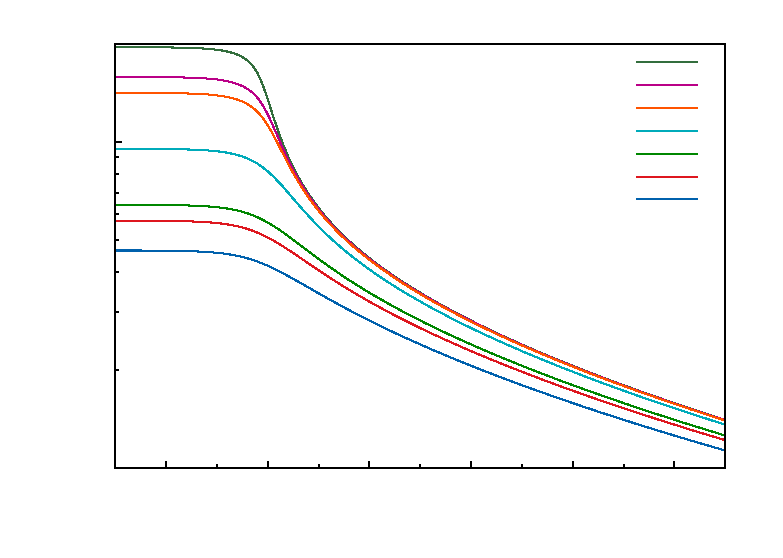
\includegraphics{./figures/size_effect_failure_stress_m10_v10}}%
    \gplfronttext
  \end{picture}%
\endgroup
}}\hfill
  \subfigure[Variation of the variance]{\scalebox{0.5}{% GNUPLOT: LaTeX picture with Postscript
\begingroup
  \makeatletter
  \providecommand\color[2][]{%
    \GenericError{(gnuplot) \space\space\space\@spaces}{%
      Package color not loaded in conjunction with
      terminal option `colourtext'%
    }{See the gnuplot documentation for explanation.%
    }{Either use 'blacktext' in gnuplot or load the package
      color.sty in LaTeX.}%
    \renewcommand\color[2][]{}%
  }%
  \providecommand\includegraphics[2][]{%
    \GenericError{(gnuplot) \space\space\space\@spaces}{%
      Package graphicx or graphics not loaded%
    }{See the gnuplot documentation for explanation.%
    }{The gnuplot epslatex terminal needs graphicx.sty or graphics.sty.}%
    \renewcommand\includegraphics[2][]{}%
  }%
  \providecommand\rotatebox[2]{#2}%
  \@ifundefined{ifGPcolor}{%
    \newif\ifGPcolor
    \GPcolorfalse
  }{}%
  \@ifundefined{ifGPblacktext}{%
    \newif\ifGPblacktext
    \GPblacktexttrue
  }{}%
  % define a \g@addto@macro without @ in the name:
  \let\gplgaddtomacro\g@addto@macro
  % define empty templates for all commands taking text:
  \gdef\gplbacktext{}%
  \gdef\gplfronttext{}%
  \makeatother
  \ifGPblacktext
    % no textcolor at all
    \def\colorrgb#1{}%
    \def\colorgray#1{}%
  \else
    % gray or color?
    \ifGPcolor
      \def\colorrgb#1{\color[rgb]{#1}}%
      \def\colorgray#1{\color[gray]{#1}}%
      \expandafter\def\csname LTw\endcsname{\color{white}}%
      \expandafter\def\csname LTb\endcsname{\color{black}}%
      \expandafter\def\csname LTa\endcsname{\color{black}}%
      \expandafter\def\csname LT0\endcsname{\color[rgb]{1,0,0}}%
      \expandafter\def\csname LT1\endcsname{\color[rgb]{0,1,0}}%
      \expandafter\def\csname LT2\endcsname{\color[rgb]{0,0,1}}%
      \expandafter\def\csname LT3\endcsname{\color[rgb]{1,0,1}}%
      \expandafter\def\csname LT4\endcsname{\color[rgb]{0,1,1}}%
      \expandafter\def\csname LT5\endcsname{\color[rgb]{1,1,0}}%
      \expandafter\def\csname LT6\endcsname{\color[rgb]{0,0,0}}%
      \expandafter\def\csname LT7\endcsname{\color[rgb]{1,0.3,0}}%
      \expandafter\def\csname LT8\endcsname{\color[rgb]{0.5,0.5,0.5}}%
    \else
      % gray
      \def\colorrgb#1{\color{black}}%
      \def\colorgray#1{\color[gray]{#1}}%
      \expandafter\def\csname LTw\endcsname{\color{white}}%
      \expandafter\def\csname LTb\endcsname{\color{black}}%
      \expandafter\def\csname LTa\endcsname{\color{black}}%
      \expandafter\def\csname LT0\endcsname{\color{black}}%
      \expandafter\def\csname LT1\endcsname{\color{black}}%
      \expandafter\def\csname LT2\endcsname{\color{black}}%
      \expandafter\def\csname LT3\endcsname{\color{black}}%
      \expandafter\def\csname LT4\endcsname{\color{black}}%
      \expandafter\def\csname LT5\endcsname{\color{black}}%
      \expandafter\def\csname LT6\endcsname{\color{black}}%
      \expandafter\def\csname LT7\endcsname{\color{black}}%
      \expandafter\def\csname LT8\endcsname{\color{black}}%
    \fi
  \fi
  \setlength{\unitlength}{0.0500bp}%
  \begin{picture}(7200.00,5040.00)%
    \gplgaddtomacro\gplbacktext{%
      \csname LTb\endcsname%
      \put(814,704){\makebox(0,0)[r]{\strut{} 1}}%
      \put(814,4775){\makebox(0,0)[r]{\strut{} 10}}%
      \put(1434,484){\makebox(0,0){\strut{} 0.01}}%
      \put(2410,484){\makebox(0,0){\strut{} 1}}%
      \put(3386,484){\makebox(0,0){\strut{} 100}}%
      \put(4363,484){\makebox(0,0){\strut{} 10000}}%
      \put(5339,484){\makebox(0,0){\strut{} 1e+06}}%
      \put(6315,484){\makebox(0,0){\strut{} 1e+08}}%
      \put(176,2739){\rotatebox{90}{\makebox(0,0){\strut{}Failure stress}}}%
      \put(3874,154){\makebox(0,0){\strut{}Scale ratio $\Msize/\Lc$}}%
    }%
    \gplgaddtomacro\gplfronttext{%
      \csname LTb\endcsname%
      \put(5816,4602){\makebox(0,0)[r]{\strut{}$\stdln^2=10$}}%
      \csname LTb\endcsname%
      \put(5816,4382){\makebox(0,0)[r]{\strut{}$\stdln^2=5$}}%
      \csname LTb\endcsname%
      \put(5816,4162){\makebox(0,0)[r]{\strut{}$\stdln^2=1$}}%
    }%
    \gplbacktext
    \put(0,0){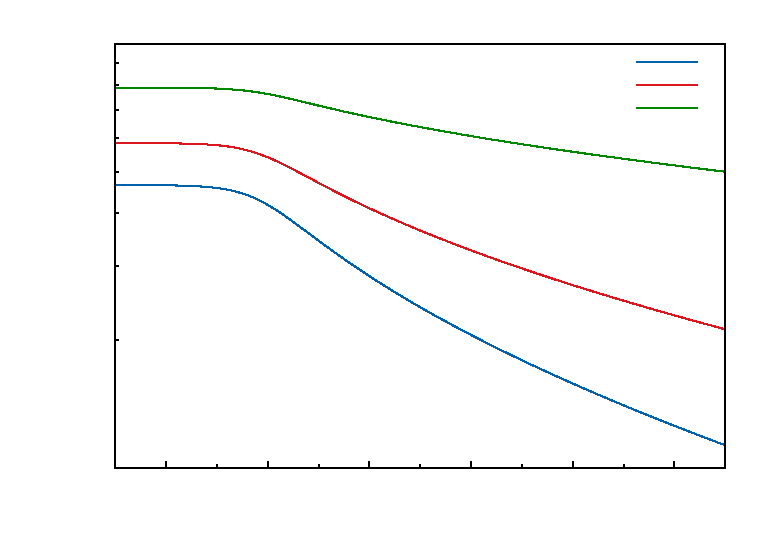
\includegraphics{./figures/size_effect_failure_stress_m10_q001}}%
    \gplfronttext
  \end{picture}%
\endgroup
}} \hfill
  \subfigure[Variation of the mean]{\scalebox{0.5}{% GNUPLOT: LaTeX picture with Postscript
\begingroup
  \makeatletter
  \providecommand\color[2][]{%
    \GenericError{(gnuplot) \space\space\space\@spaces}{%
      Package color not loaded in conjunction with
      terminal option `colourtext'%
    }{See the gnuplot documentation for explanation.%
    }{Either use 'blacktext' in gnuplot or load the package
      color.sty in LaTeX.}%
    \renewcommand\color[2][]{}%
  }%
  \providecommand\includegraphics[2][]{%
    \GenericError{(gnuplot) \space\space\space\@spaces}{%
      Package graphicx or graphics not loaded%
    }{See the gnuplot documentation for explanation.%
    }{The gnuplot epslatex terminal needs graphicx.sty or graphics.sty.}%
    \renewcommand\includegraphics[2][]{}%
  }%
  \providecommand\rotatebox[2]{#2}%
  \@ifundefined{ifGPcolor}{%
    \newif\ifGPcolor
    \GPcolorfalse
  }{}%
  \@ifundefined{ifGPblacktext}{%
    \newif\ifGPblacktext
    \GPblacktexttrue
  }{}%
  % define a \g@addto@macro without @ in the name:
  \let\gplgaddtomacro\g@addto@macro
  % define empty templates for all commands taking text:
  \gdef\gplbacktext{}%
  \gdef\gplfronttext{}%
  \makeatother
  \ifGPblacktext
    % no textcolor at all
    \def\colorrgb#1{}%
    \def\colorgray#1{}%
  \else
    % gray or color?
    \ifGPcolor
      \def\colorrgb#1{\color[rgb]{#1}}%
      \def\colorgray#1{\color[gray]{#1}}%
      \expandafter\def\csname LTw\endcsname{\color{white}}%
      \expandafter\def\csname LTb\endcsname{\color{black}}%
      \expandafter\def\csname LTa\endcsname{\color{black}}%
      \expandafter\def\csname LT0\endcsname{\color[rgb]{1,0,0}}%
      \expandafter\def\csname LT1\endcsname{\color[rgb]{0,1,0}}%
      \expandafter\def\csname LT2\endcsname{\color[rgb]{0,0,1}}%
      \expandafter\def\csname LT3\endcsname{\color[rgb]{1,0,1}}%
      \expandafter\def\csname LT4\endcsname{\color[rgb]{0,1,1}}%
      \expandafter\def\csname LT5\endcsname{\color[rgb]{1,1,0}}%
      \expandafter\def\csname LT6\endcsname{\color[rgb]{0,0,0}}%
      \expandafter\def\csname LT7\endcsname{\color[rgb]{1,0.3,0}}%
      \expandafter\def\csname LT8\endcsname{\color[rgb]{0.5,0.5,0.5}}%
    \else
      % gray
      \def\colorrgb#1{\color{black}}%
      \def\colorgray#1{\color[gray]{#1}}%
      \expandafter\def\csname LTw\endcsname{\color{white}}%
      \expandafter\def\csname LTb\endcsname{\color{black}}%
      \expandafter\def\csname LTa\endcsname{\color{black}}%
      \expandafter\def\csname LT0\endcsname{\color{black}}%
      \expandafter\def\csname LT1\endcsname{\color{black}}%
      \expandafter\def\csname LT2\endcsname{\color{black}}%
      \expandafter\def\csname LT3\endcsname{\color{black}}%
      \expandafter\def\csname LT4\endcsname{\color{black}}%
      \expandafter\def\csname LT5\endcsname{\color{black}}%
      \expandafter\def\csname LT6\endcsname{\color{black}}%
      \expandafter\def\csname LT7\endcsname{\color{black}}%
      \expandafter\def\csname LT8\endcsname{\color{black}}%
    \fi
  \fi
  \setlength{\unitlength}{0.0500bp}%
  \begin{picture}(7200.00,5040.00)%
    \gplgaddtomacro\gplbacktext{%
      \csname LTb\endcsname%
      \put(1210,704){\makebox(0,0)[r]{\strut{} 0.001}}%
      \put(1210,1722){\makebox(0,0)[r]{\strut{} 0.01}}%
      \put(1210,2740){\makebox(0,0)[r]{\strut{} 0.1}}%
      \put(1210,3757){\makebox(0,0)[r]{\strut{} 1}}%
      \put(1210,4775){\makebox(0,0)[r]{\strut{} 10}}%
      \put(1797,484){\makebox(0,0){\strut{} 0.01}}%
      \put(2707,484){\makebox(0,0){\strut{} 1}}%
      \put(3617,484){\makebox(0,0){\strut{} 100}}%
      \put(4528,484){\makebox(0,0){\strut{} 10000}}%
      \put(5438,484){\makebox(0,0){\strut{} 1e+06}}%
      \put(6348,484){\makebox(0,0){\strut{} 1e+08}}%
      \put(176,2739){\rotatebox{90}{\makebox(0,0){\strut{}Failure stress}}}%
      \put(4072,154){\makebox(0,0){\strut{}Scale ratio $\Msize/\Lc$}}%
    }%
    \gplgaddtomacro\gplfronttext{%
      \csname LTb\endcsname%
      \put(5816,4602){\makebox(0,0)[r]{\strut{}$\meanln=10$}}%
      \csname LTb\endcsname%
      \put(5816,4382){\makebox(0,0)[r]{\strut{}$\meanln=5$}}%
      \csname LTb\endcsname%
      \put(5816,4162){\makebox(0,0)[r]{\strut{}$\meanln=1$}}%
    }%
    \gplbacktext
    \put(0,0){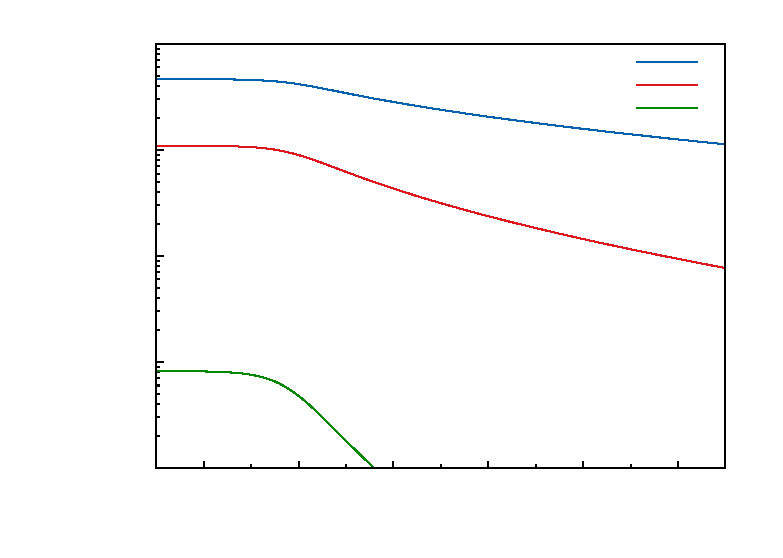
\includegraphics{./figures/size_effect_failure_stress_v10_q001}}%
    \gplfronttext
  \end{picture}%
\endgroup
}}\hspace*{\fill}
  \caption{Size Effect: variations around $\meanln=10$, $\stdln^2=10$ and $q=1\%$ in 1D.}
\end{figure}

\subsection{Two dimensional case}
\begin{figure}[!h]
  \centering
  \hspace*{\fill}
  \subfigure[$\Msize=0.001$\label{fig:2D:EC:small_size}]{\scalebox{0.5}{% GNUPLOT: LaTeX picture with Postscript
\begingroup
  \makeatletter
  \providecommand\color[2][]{%
    \GenericError{(gnuplot) \space\space\space\@spaces}{%
      Package color not loaded in conjunction with
      terminal option `colourtext'%
    }{See the gnuplot documentation for explanation.%
    }{Either use 'blacktext' in gnuplot or load the package
      color.sty in LaTeX.}%
    \renewcommand\color[2][]{}%
  }%
  \providecommand\includegraphics[2][]{%
    \GenericError{(gnuplot) \space\space\space\@spaces}{%
      Package graphicx or graphics not loaded%
    }{See the gnuplot documentation for explanation.%
    }{The gnuplot epslatex terminal needs graphicx.sty or graphics.sty.}%
    \renewcommand\includegraphics[2][]{}%
  }%
  \providecommand\rotatebox[2]{#2}%
  \@ifundefined{ifGPcolor}{%
    \newif\ifGPcolor
    \GPcolorfalse
  }{}%
  \@ifundefined{ifGPblacktext}{%
    \newif\ifGPblacktext
    \GPblacktexttrue
  }{}%
  % define a \g@addto@macro without @ in the name:
  \let\gplgaddtomacro\g@addto@macro
  % define empty templates for all commands taking text:
  \gdef\gplbacktext{}%
  \gdef\gplfronttext{}%
  \makeatother
  \ifGPblacktext
    % no textcolor at all
    \def\colorrgb#1{}%
    \def\colorgray#1{}%
  \else
    % gray or color?
    \ifGPcolor
      \def\colorrgb#1{\color[rgb]{#1}}%
      \def\colorgray#1{\color[gray]{#1}}%
      \expandafter\def\csname LTw\endcsname{\color{white}}%
      \expandafter\def\csname LTb\endcsname{\color{black}}%
      \expandafter\def\csname LTa\endcsname{\color{black}}%
      \expandafter\def\csname LT0\endcsname{\color[rgb]{1,0,0}}%
      \expandafter\def\csname LT1\endcsname{\color[rgb]{0,1,0}}%
      \expandafter\def\csname LT2\endcsname{\color[rgb]{0,0,1}}%
      \expandafter\def\csname LT3\endcsname{\color[rgb]{1,0,1}}%
      \expandafter\def\csname LT4\endcsname{\color[rgb]{0,1,1}}%
      \expandafter\def\csname LT5\endcsname{\color[rgb]{1,1,0}}%
      \expandafter\def\csname LT6\endcsname{\color[rgb]{0,0,0}}%
      \expandafter\def\csname LT7\endcsname{\color[rgb]{1,0.3,0}}%
      \expandafter\def\csname LT8\endcsname{\color[rgb]{0.5,0.5,0.5}}%
    \else
      % gray
      \def\colorrgb#1{\color{black}}%
      \def\colorgray#1{\color[gray]{#1}}%
      \expandafter\def\csname LTw\endcsname{\color{white}}%
      \expandafter\def\csname LTb\endcsname{\color{black}}%
      \expandafter\def\csname LTa\endcsname{\color{black}}%
      \expandafter\def\csname LT0\endcsname{\color{black}}%
      \expandafter\def\csname LT1\endcsname{\color{black}}%
      \expandafter\def\csname LT2\endcsname{\color{black}}%
      \expandafter\def\csname LT3\endcsname{\color{black}}%
      \expandafter\def\csname LT4\endcsname{\color{black}}%
      \expandafter\def\csname LT5\endcsname{\color{black}}%
      \expandafter\def\csname LT6\endcsname{\color{black}}%
      \expandafter\def\csname LT7\endcsname{\color{black}}%
      \expandafter\def\csname LT8\endcsname{\color{black}}%
    \fi
  \fi
  \setlength{\unitlength}{0.0500bp}%
  \begin{picture}(7200.00,5040.00)%
    \gplgaddtomacro\gplbacktext{%
      \csname LTb\endcsname%
      \put(946,704){\makebox(0,0)[r]{\strut{} 0}}%
      \put(946,1111){\makebox(0,0)[r]{\strut{} 0.1}}%
      \put(946,1518){\makebox(0,0)[r]{\strut{} 0.2}}%
      \put(946,1925){\makebox(0,0)[r]{\strut{} 0.3}}%
      \put(946,2332){\makebox(0,0)[r]{\strut{} 0.4}}%
      \put(946,2740){\makebox(0,0)[r]{\strut{} 0.5}}%
      \put(946,3147){\makebox(0,0)[r]{\strut{} 0.6}}%
      \put(946,3554){\makebox(0,0)[r]{\strut{} 0.7}}%
      \put(946,3961){\makebox(0,0)[r]{\strut{} 0.8}}%
      \put(946,4368){\makebox(0,0)[r]{\strut{} 0.9}}%
      \put(946,4775){\makebox(0,0)[r]{\strut{} 1}}%
      \put(1078,484){\makebox(0,0){\strut{} 0.001}}%
      \put(2223,484){\makebox(0,0){\strut{} 0.01}}%
      \put(3368,484){\makebox(0,0){\strut{} 0.1}}%
      \put(4513,484){\makebox(0,0){\strut{} 1}}%
      \put(5658,484){\makebox(0,0){\strut{} 10}}%
      \put(6803,484){\makebox(0,0){\strut{} 100}}%
      \csname LTb\endcsname%
      \put(176,2739){\rotatebox{90}{\makebox(0,0){\strut{}Euler characteristic $\EC$}}}%
      \put(3940,154){\makebox(0,0){\strut{}$\lset$}}%
    }%
    \gplgaddtomacro\gplfronttext{%
    }%
    \gplbacktext
    \put(0,0){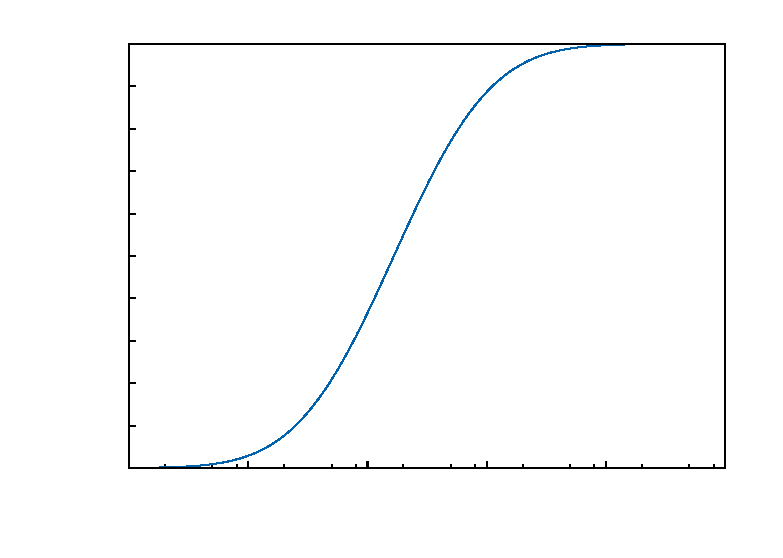
\includegraphics{./figures/size_effect_2D_different_Euler_behaviors_l0.001.eps}}%
    \gplfronttext
  \end{picture}%
\endgroup
}}\hfill
%  \subfigure[$\Msize=0.8$]  {\scalebox{0.5}{% GNUPLOT: LaTeX picture with Postscript
\begingroup
  \makeatletter
  \providecommand\color[2][]{%
    \GenericError{(gnuplot) \space\space\space\@spaces}{%
      Package color not loaded in conjunction with
      terminal option `colourtext'%
    }{See the gnuplot documentation for explanation.%
    }{Either use 'blacktext' in gnuplot or load the package
      color.sty in LaTeX.}%
    \renewcommand\color[2][]{}%
  }%
  \providecommand\includegraphics[2][]{%
    \GenericError{(gnuplot) \space\space\space\@spaces}{%
      Package graphicx or graphics not loaded%
    }{See the gnuplot documentation for explanation.%
    }{The gnuplot epslatex terminal needs graphicx.sty or graphics.sty.}%
    \renewcommand\includegraphics[2][]{}%
  }%
  \providecommand\rotatebox[2]{#2}%
  \@ifundefined{ifGPcolor}{%
    \newif\ifGPcolor
    \GPcolorfalse
  }{}%
  \@ifundefined{ifGPblacktext}{%
    \newif\ifGPblacktext
    \GPblacktexttrue
  }{}%
  % define a \g@addto@macro without @ in the name:
  \let\gplgaddtomacro\g@addto@macro
  % define empty templates for all commands taking text:
  \gdef\gplbacktext{}%
  \gdef\gplfronttext{}%
  \makeatother
  \ifGPblacktext
    % no textcolor at all
    \def\colorrgb#1{}%
    \def\colorgray#1{}%
  \else
    % gray or color?
    \ifGPcolor
      \def\colorrgb#1{\color[rgb]{#1}}%
      \def\colorgray#1{\color[gray]{#1}}%
      \expandafter\def\csname LTw\endcsname{\color{white}}%
      \expandafter\def\csname LTb\endcsname{\color{black}}%
      \expandafter\def\csname LTa\endcsname{\color{black}}%
      \expandafter\def\csname LT0\endcsname{\color[rgb]{1,0,0}}%
      \expandafter\def\csname LT1\endcsname{\color[rgb]{0,1,0}}%
      \expandafter\def\csname LT2\endcsname{\color[rgb]{0,0,1}}%
      \expandafter\def\csname LT3\endcsname{\color[rgb]{1,0,1}}%
      \expandafter\def\csname LT4\endcsname{\color[rgb]{0,1,1}}%
      \expandafter\def\csname LT5\endcsname{\color[rgb]{1,1,0}}%
      \expandafter\def\csname LT6\endcsname{\color[rgb]{0,0,0}}%
      \expandafter\def\csname LT7\endcsname{\color[rgb]{1,0.3,0}}%
      \expandafter\def\csname LT8\endcsname{\color[rgb]{0.5,0.5,0.5}}%
    \else
      % gray
      \def\colorrgb#1{\color{black}}%
      \def\colorgray#1{\color[gray]{#1}}%
      \expandafter\def\csname LTw\endcsname{\color{white}}%
      \expandafter\def\csname LTb\endcsname{\color{black}}%
      \expandafter\def\csname LTa\endcsname{\color{black}}%
      \expandafter\def\csname LT0\endcsname{\color{black}}%
      \expandafter\def\csname LT1\endcsname{\color{black}}%
      \expandafter\def\csname LT2\endcsname{\color{black}}%
      \expandafter\def\csname LT3\endcsname{\color{black}}%
      \expandafter\def\csname LT4\endcsname{\color{black}}%
      \expandafter\def\csname LT5\endcsname{\color{black}}%
      \expandafter\def\csname LT6\endcsname{\color{black}}%
      \expandafter\def\csname LT7\endcsname{\color{black}}%
      \expandafter\def\csname LT8\endcsname{\color{black}}%
    \fi
  \fi
  \setlength{\unitlength}{0.0500bp}%
  \begin{picture}(7200.00,5040.00)%
    \gplgaddtomacro\gplbacktext{%
      \csname LTb\endcsname%
      \put(946,704){\makebox(0,0)[r]{\strut{} 0}}%
      \put(946,1383){\makebox(0,0)[r]{\strut{} 0.2}}%
      \put(946,2061){\makebox(0,0)[r]{\strut{} 0.4}}%
      \put(946,2740){\makebox(0,0)[r]{\strut{} 0.6}}%
      \put(946,3418){\makebox(0,0)[r]{\strut{} 0.8}}%
      \put(946,4097){\makebox(0,0)[r]{\strut{} 1}}%
      \put(946,4775){\makebox(0,0)[r]{\strut{} 1.2}}%
      \put(1078,484){\makebox(0,0){\strut{} 0.001}}%
      \put(2223,484){\makebox(0,0){\strut{} 0.01}}%
      \put(3368,484){\makebox(0,0){\strut{} 0.1}}%
      \put(4513,484){\makebox(0,0){\strut{} 1}}%
      \put(5658,484){\makebox(0,0){\strut{} 10}}%
      \put(6803,484){\makebox(0,0){\strut{} 100}}%
      \csname LTb\endcsname%
      \put(176,2739){\rotatebox{90}{\makebox(0,0){\strut{}Euler characteristic}}}%
      \put(3940,154){\makebox(0,0){\strut{}$\lset$}}%
    }%
    \gplgaddtomacro\gplfronttext{%
    }%
    \gplbacktext
    \put(0,0){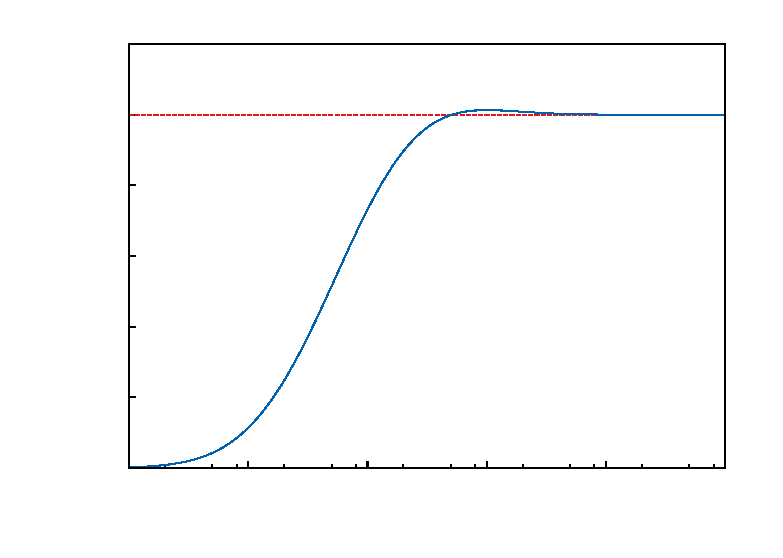
\includegraphics{./figures/size_effect_2D_different_Euler_behaviors_l0.8.eps}}%
    \gplfronttext
  \end{picture}%
\endgroup
}}\\
  \subfigure[$\Msize=2.5$\label{fig:2D:EC:medium_size}]  {\scalebox{0.5}{% GNUPLOT: LaTeX picture with Postscript
\begingroup
  \makeatletter
  \providecommand\color[2][]{%
    \GenericError{(gnuplot) \space\space\space\@spaces}{%
      Package color not loaded in conjunction with
      terminal option `colourtext'%
    }{See the gnuplot documentation for explanation.%
    }{Either use 'blacktext' in gnuplot or load the package
      color.sty in LaTeX.}%
    \renewcommand\color[2][]{}%
  }%
  \providecommand\includegraphics[2][]{%
    \GenericError{(gnuplot) \space\space\space\@spaces}{%
      Package graphicx or graphics not loaded%
    }{See the gnuplot documentation for explanation.%
    }{The gnuplot epslatex terminal needs graphicx.sty or graphics.sty.}%
    \renewcommand\includegraphics[2][]{}%
  }%
  \providecommand\rotatebox[2]{#2}%
  \@ifundefined{ifGPcolor}{%
    \newif\ifGPcolor
    \GPcolorfalse
  }{}%
  \@ifundefined{ifGPblacktext}{%
    \newif\ifGPblacktext
    \GPblacktexttrue
  }{}%
  % define a \g@addto@macro without @ in the name:
  \let\gplgaddtomacro\g@addto@macro
  % define empty templates for all commands taking text:
  \gdef\gplbacktext{}%
  \gdef\gplfronttext{}%
  \makeatother
  \ifGPblacktext
    % no textcolor at all
    \def\colorrgb#1{}%
    \def\colorgray#1{}%
  \else
    % gray or color?
    \ifGPcolor
      \def\colorrgb#1{\color[rgb]{#1}}%
      \def\colorgray#1{\color[gray]{#1}}%
      \expandafter\def\csname LTw\endcsname{\color{white}}%
      \expandafter\def\csname LTb\endcsname{\color{black}}%
      \expandafter\def\csname LTa\endcsname{\color{black}}%
      \expandafter\def\csname LT0\endcsname{\color[rgb]{1,0,0}}%
      \expandafter\def\csname LT1\endcsname{\color[rgb]{0,1,0}}%
      \expandafter\def\csname LT2\endcsname{\color[rgb]{0,0,1}}%
      \expandafter\def\csname LT3\endcsname{\color[rgb]{1,0,1}}%
      \expandafter\def\csname LT4\endcsname{\color[rgb]{0,1,1}}%
      \expandafter\def\csname LT5\endcsname{\color[rgb]{1,1,0}}%
      \expandafter\def\csname LT6\endcsname{\color[rgb]{0,0,0}}%
      \expandafter\def\csname LT7\endcsname{\color[rgb]{1,0.3,0}}%
      \expandafter\def\csname LT8\endcsname{\color[rgb]{0.5,0.5,0.5}}%
    \else
      % gray
      \def\colorrgb#1{\color{black}}%
      \def\colorgray#1{\color[gray]{#1}}%
      \expandafter\def\csname LTw\endcsname{\color{white}}%
      \expandafter\def\csname LTb\endcsname{\color{black}}%
      \expandafter\def\csname LTa\endcsname{\color{black}}%
      \expandafter\def\csname LT0\endcsname{\color{black}}%
      \expandafter\def\csname LT1\endcsname{\color{black}}%
      \expandafter\def\csname LT2\endcsname{\color{black}}%
      \expandafter\def\csname LT3\endcsname{\color{black}}%
      \expandafter\def\csname LT4\endcsname{\color{black}}%
      \expandafter\def\csname LT5\endcsname{\color{black}}%
      \expandafter\def\csname LT6\endcsname{\color{black}}%
      \expandafter\def\csname LT7\endcsname{\color{black}}%
      \expandafter\def\csname LT8\endcsname{\color{black}}%
    \fi
  \fi
  \setlength{\unitlength}{0.0500bp}%
  \begin{picture}(7200.00,5040.00)%
    \gplgaddtomacro\gplbacktext{%
      \csname LTb\endcsname%
      \put(946,704){\makebox(0,0)[r]{\strut{} 0}}%
      \put(946,1156){\makebox(0,0)[r]{\strut{} 0.2}}%
      \put(946,1609){\makebox(0,0)[r]{\strut{} 0.4}}%
      \put(946,2061){\makebox(0,0)[r]{\strut{} 0.6}}%
      \put(946,2513){\makebox(0,0)[r]{\strut{} 0.8}}%
      \put(946,2966){\makebox(0,0)[r]{\strut{} 1}}%
      \put(946,3418){\makebox(0,0)[r]{\strut{} 1.2}}%
      \put(946,3870){\makebox(0,0)[r]{\strut{} 1.4}}%
      \put(946,4323){\makebox(0,0)[r]{\strut{} 1.6}}%
      \put(946,4775){\makebox(0,0)[r]{\strut{} 1.8}}%
      \put(1078,484){\makebox(0,0){\strut{} 0.001}}%
      \put(2223,484){\makebox(0,0){\strut{} 0.01}}%
      \put(3368,484){\makebox(0,0){\strut{} 0.1}}%
      \put(4513,484){\makebox(0,0){\strut{} 1}}%
      \put(5658,484){\makebox(0,0){\strut{} 10}}%
      \put(6803,484){\makebox(0,0){\strut{} 100}}%
      \csname LTb\endcsname%
      \put(176,2739){\rotatebox{90}{\makebox(0,0){\strut{}Euler characteristic}}}%
      \put(3940,154){\makebox(0,0){\strut{}$\lset$}}%
    }%
    \gplgaddtomacro\gplfronttext{%
    }%
    \gplbacktext
    \put(0,0){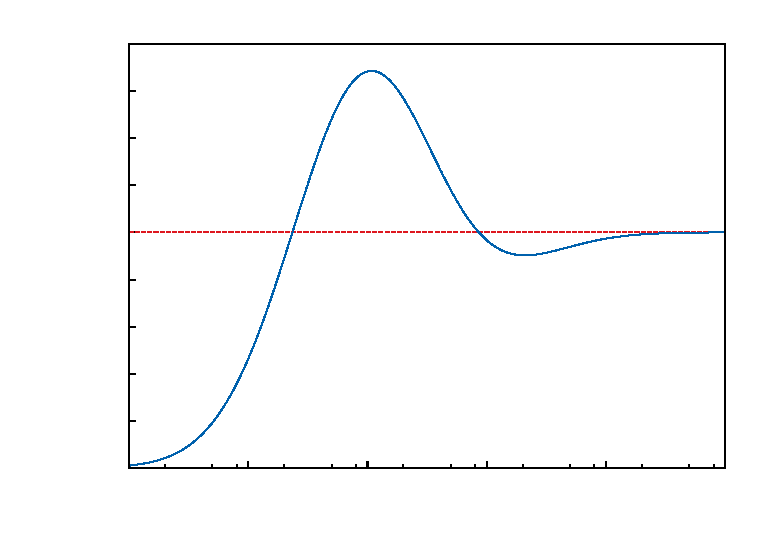
\includegraphics{./figures/size_effect_2D_different_Euler_behaviors_l2.5}}%
    \gplfronttext
  \end{picture}%
\endgroup
}}\hfill
  \subfigure[$\Msize=8$\label{fig:2D:EC:large_size}]    {\scalebox{0.5}{% GNUPLOT: LaTeX picture with Postscript
\begingroup
  \makeatletter
  \providecommand\color[2][]{%
    \GenericError{(gnuplot) \space\space\space\@spaces}{%
      Package color not loaded in conjunction with
      terminal option `colourtext'%
    }{See the gnuplot documentation for explanation.%
    }{Either use 'blacktext' in gnuplot or load the package
      color.sty in LaTeX.}%
    \renewcommand\color[2][]{}%
  }%
  \providecommand\includegraphics[2][]{%
    \GenericError{(gnuplot) \space\space\space\@spaces}{%
      Package graphicx or graphics not loaded%
    }{See the gnuplot documentation for explanation.%
    }{The gnuplot epslatex terminal needs graphicx.sty or graphics.sty.}%
    \renewcommand\includegraphics[2][]{}%
  }%
  \providecommand\rotatebox[2]{#2}%
  \@ifundefined{ifGPcolor}{%
    \newif\ifGPcolor
    \GPcolorfalse
  }{}%
  \@ifundefined{ifGPblacktext}{%
    \newif\ifGPblacktext
    \GPblacktexttrue
  }{}%
  % define a \g@addto@macro without @ in the name:
  \let\gplgaddtomacro\g@addto@macro
  % define empty templates for all commands taking text:
  \gdef\gplbacktext{}%
  \gdef\gplfronttext{}%
  \makeatother
  \ifGPblacktext
    % no textcolor at all
    \def\colorrgb#1{}%
    \def\colorgray#1{}%
  \else
    % gray or color?
    \ifGPcolor
      \def\colorrgb#1{\color[rgb]{#1}}%
      \def\colorgray#1{\color[gray]{#1}}%
      \expandafter\def\csname LTw\endcsname{\color{white}}%
      \expandafter\def\csname LTb\endcsname{\color{black}}%
      \expandafter\def\csname LTa\endcsname{\color{black}}%
      \expandafter\def\csname LT0\endcsname{\color[rgb]{1,0,0}}%
      \expandafter\def\csname LT1\endcsname{\color[rgb]{0,1,0}}%
      \expandafter\def\csname LT2\endcsname{\color[rgb]{0,0,1}}%
      \expandafter\def\csname LT3\endcsname{\color[rgb]{1,0,1}}%
      \expandafter\def\csname LT4\endcsname{\color[rgb]{0,1,1}}%
      \expandafter\def\csname LT5\endcsname{\color[rgb]{1,1,0}}%
      \expandafter\def\csname LT6\endcsname{\color[rgb]{0,0,0}}%
      \expandafter\def\csname LT7\endcsname{\color[rgb]{1,0.3,0}}%
      \expandafter\def\csname LT8\endcsname{\color[rgb]{0.5,0.5,0.5}}%
    \else
      % gray
      \def\colorrgb#1{\color{black}}%
      \def\colorgray#1{\color[gray]{#1}}%
      \expandafter\def\csname LTw\endcsname{\color{white}}%
      \expandafter\def\csname LTb\endcsname{\color{black}}%
      \expandafter\def\csname LTa\endcsname{\color{black}}%
      \expandafter\def\csname LT0\endcsname{\color{black}}%
      \expandafter\def\csname LT1\endcsname{\color{black}}%
      \expandafter\def\csname LT2\endcsname{\color{black}}%
      \expandafter\def\csname LT3\endcsname{\color{black}}%
      \expandafter\def\csname LT4\endcsname{\color{black}}%
      \expandafter\def\csname LT5\endcsname{\color{black}}%
      \expandafter\def\csname LT6\endcsname{\color{black}}%
      \expandafter\def\csname LT7\endcsname{\color{black}}%
      \expandafter\def\csname LT8\endcsname{\color{black}}%
    \fi
  \fi
  \setlength{\unitlength}{0.0500bp}%
  \begin{picture}(7200.00,5040.00)%
    \gplgaddtomacro\gplbacktext{%
      \csname LTb\endcsname%
      \put(682,704){\makebox(0,0)[r]{\strut{}-3}}%
      \put(682,1074){\makebox(0,0)[r]{\strut{}-2}}%
      \put(682,1444){\makebox(0,0)[r]{\strut{}-1}}%
      \put(682,1814){\makebox(0,0)[r]{\strut{} 0}}%
      \put(682,2184){\makebox(0,0)[r]{\strut{} 1}}%
      \put(682,2554){\makebox(0,0)[r]{\strut{} 2}}%
      \put(682,2925){\makebox(0,0)[r]{\strut{} 3}}%
      \put(682,3295){\makebox(0,0)[r]{\strut{} 4}}%
      \put(682,3665){\makebox(0,0)[r]{\strut{} 5}}%
      \put(682,4035){\makebox(0,0)[r]{\strut{} 6}}%
      \put(682,4405){\makebox(0,0)[r]{\strut{} 7}}%
      \put(682,4775){\makebox(0,0)[r]{\strut{} 8}}%
      \put(814,484){\makebox(0,0){\strut{} 0.001}}%
      \put(2012,484){\makebox(0,0){\strut{} 0.01}}%
      \put(3210,484){\makebox(0,0){\strut{} 0.1}}%
      \put(4407,484){\makebox(0,0){\strut{} 1}}%
      \put(5605,484){\makebox(0,0){\strut{} 10}}%
      \put(6803,484){\makebox(0,0){\strut{} 100}}%
      \csname LTb\endcsname%
      \put(176,2739){\rotatebox{90}{\makebox(0,0){\strut{}Euler characteristic $\EC$}}}%
      \put(3808,154){\makebox(0,0){\strut{}$\lset$}}%
    }%
    \gplgaddtomacro\gplfronttext{%
    }%
    \gplbacktext
    \put(0,0){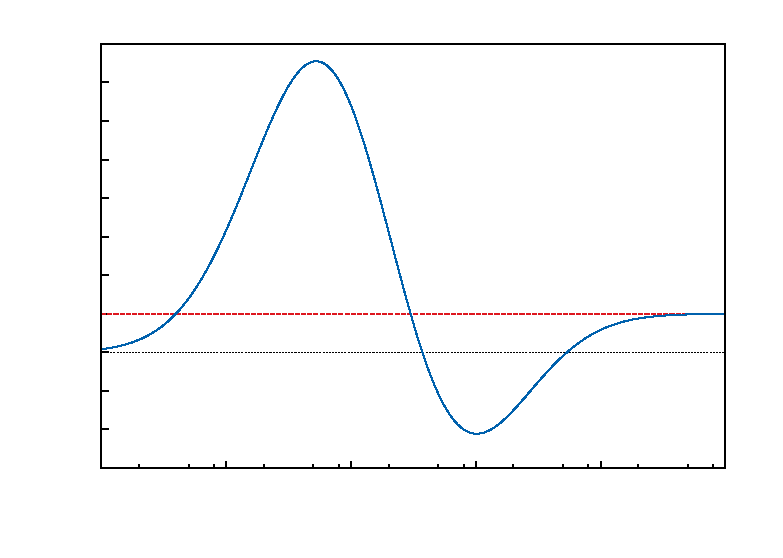
\includegraphics{./figures/size_effect_2D_different_Euler_behaviors_l8.eps}}%
    \gplfronttext
  \end{picture}%
\endgroup
}}  \hspace*{\fill}
  \caption{Euler characteristic for different specimen sizes $\Msize$ for $\meanln=0.5$, $\stdln^2=2$, $\Lc=1$, and $\HS=\zu$ (lognormal distribution with cumulative hitting set) in a 2D.\label{fig:2D:EC}}
\end{figure}

\begin{itemize}
  \item [\ref{fig:2D:EC:small_size}] Small sizes \\ \textbf{Direct percolation}. The first (and only) $\lset(\EC==q)$ correspond to the probability $q$ of percolation. There is only one disconnected element in the excursion set.
  \item [\ref{fig:2D:EC:medium_size}] Medium sizes \\ 
  \item [\ref{fig:2D:EC:large_size}] Large sizes \\ 
\end{itemize}


\subsection{Three dimensional case}
\begin{figure}[!h]
  \centering
    \hspace*{\fill}
  \subfigure{\scalebox{0.5}{% GNUPLOT: LaTeX picture with Postscript
\begingroup
  \makeatletter
  \providecommand\color[2][]{%
    \GenericError{(gnuplot) \space\space\space\@spaces}{%
      Package color not loaded in conjunction with
      terminal option `colourtext'%
    }{See the gnuplot documentation for explanation.%
    }{Either use 'blacktext' in gnuplot or load the package
      color.sty in LaTeX.}%
    \renewcommand\color[2][]{}%
  }%
  \providecommand\includegraphics[2][]{%
    \GenericError{(gnuplot) \space\space\space\@spaces}{%
      Package graphicx or graphics not loaded%
    }{See the gnuplot documentation for explanation.%
    }{The gnuplot epslatex terminal needs graphicx.sty or graphics.sty.}%
    \renewcommand\includegraphics[2][]{}%
  }%
  \providecommand\rotatebox[2]{#2}%
  \@ifundefined{ifGPcolor}{%
    \newif\ifGPcolor
    \GPcolorfalse
  }{}%
  \@ifundefined{ifGPblacktext}{%
    \newif\ifGPblacktext
    \GPblacktexttrue
  }{}%
  % define a \g@addto@macro without @ in the name:
  \let\gplgaddtomacro\g@addto@macro
  % define empty templates for all commands taking text:
  \gdef\gplbacktext{}%
  \gdef\gplfronttext{}%
  \makeatother
  \ifGPblacktext
    % no textcolor at all
    \def\colorrgb#1{}%
    \def\colorgray#1{}%
  \else
    % gray or color?
    \ifGPcolor
      \def\colorrgb#1{\color[rgb]{#1}}%
      \def\colorgray#1{\color[gray]{#1}}%
      \expandafter\def\csname LTw\endcsname{\color{white}}%
      \expandafter\def\csname LTb\endcsname{\color{black}}%
      \expandafter\def\csname LTa\endcsname{\color{black}}%
      \expandafter\def\csname LT0\endcsname{\color[rgb]{1,0,0}}%
      \expandafter\def\csname LT1\endcsname{\color[rgb]{0,1,0}}%
      \expandafter\def\csname LT2\endcsname{\color[rgb]{0,0,1}}%
      \expandafter\def\csname LT3\endcsname{\color[rgb]{1,0,1}}%
      \expandafter\def\csname LT4\endcsname{\color[rgb]{0,1,1}}%
      \expandafter\def\csname LT5\endcsname{\color[rgb]{1,1,0}}%
      \expandafter\def\csname LT6\endcsname{\color[rgb]{0,0,0}}%
      \expandafter\def\csname LT7\endcsname{\color[rgb]{1,0.3,0}}%
      \expandafter\def\csname LT8\endcsname{\color[rgb]{0.5,0.5,0.5}}%
    \else
      % gray
      \def\colorrgb#1{\color{black}}%
      \def\colorgray#1{\color[gray]{#1}}%
      \expandafter\def\csname LTw\endcsname{\color{white}}%
      \expandafter\def\csname LTb\endcsname{\color{black}}%
      \expandafter\def\csname LTa\endcsname{\color{black}}%
      \expandafter\def\csname LT0\endcsname{\color{black}}%
      \expandafter\def\csname LT1\endcsname{\color{black}}%
      \expandafter\def\csname LT2\endcsname{\color{black}}%
      \expandafter\def\csname LT3\endcsname{\color{black}}%
      \expandafter\def\csname LT4\endcsname{\color{black}}%
      \expandafter\def\csname LT5\endcsname{\color{black}}%
      \expandafter\def\csname LT6\endcsname{\color{black}}%
      \expandafter\def\csname LT7\endcsname{\color{black}}%
      \expandafter\def\csname LT8\endcsname{\color{black}}%
    \fi
  \fi
  \setlength{\unitlength}{0.0500bp}%
  \begin{picture}(7200.00,5040.00)%
    \gplgaddtomacro\gplbacktext{%
      \csname LTb\endcsname%
      \put(946,704){\makebox(0,0)[r]{\strut{}-1.5}}%
      \put(946,1518){\makebox(0,0)[r]{\strut{}-1}}%
      \put(946,2332){\makebox(0,0)[r]{\strut{}-0.5}}%
      \put(946,3147){\makebox(0,0)[r]{\strut{} 0}}%
      \put(946,3961){\makebox(0,0)[r]{\strut{} 0.5}}%
      \put(946,4775){\makebox(0,0)[r]{\strut{} 1}}%
      \put(1078,484){\makebox(0,0){\strut{} 0.001}}%
      \put(2032,484){\makebox(0,0){\strut{} 0.01}}%
      \put(2986,484){\makebox(0,0){\strut{} 0.1}}%
      \put(3941,484){\makebox(0,0){\strut{} 1}}%
      \put(4895,484){\makebox(0,0){\strut{} 10}}%
      \put(5849,484){\makebox(0,0){\strut{} 100}}%
      \put(6803,484){\makebox(0,0){\strut{} 1000}}%
      \csname LTb\endcsname%
      \put(176,2739){\rotatebox{90}{\makebox(0,0){\strut{}Euler characteristic}}}%
      \put(3940,154){\makebox(0,0){\strut{}$\lset$}}%
    }%
    \gplgaddtomacro\gplfronttext{%
      \csname LTb\endcsname%
      \put(5816,1317){\makebox(0,0)[r]{\strut{}$100\times 10\times 10$}}%
      \csname LTb\endcsname%
      \put(5816,1097){\makebox(0,0)[r]{\strut{}$200\times 20\times 20$}}%
      \csname LTb\endcsname%
      \put(5816,877){\makebox(0,0)[r]{\strut{}$400\times 40\times 40$}}%
    }%
    \gplbacktext
    \put(0,0){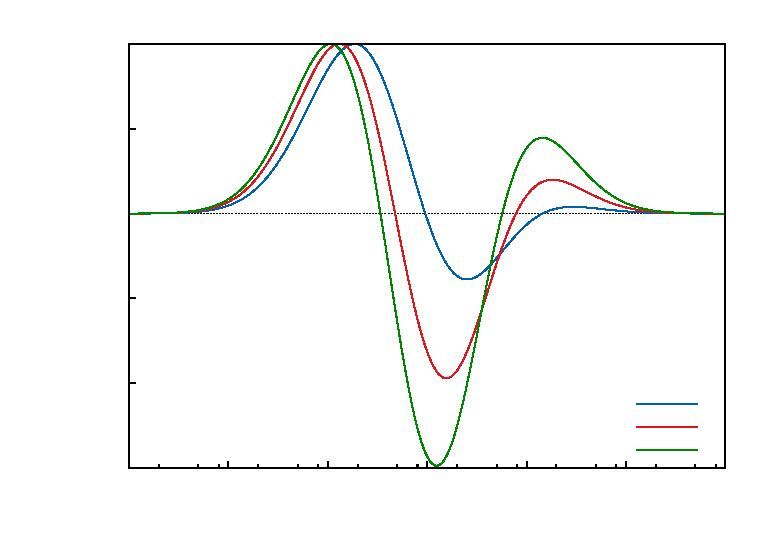
\includegraphics{./figures/elkc_th_3D_lognormal_0_constant_ratio}}%
    \gplfronttext
  \end{picture}%
\endgroup
}}\hfill
  \subfigure{\scalebox{0.5}{% GNUPLOT: LaTeX picture with Postscript
\begingroup
  \makeatletter
  \providecommand\color[2][]{%
    \GenericError{(gnuplot) \space\space\space\@spaces}{%
      Package color not loaded in conjunction with
      terminal option `colourtext'%
    }{See the gnuplot documentation for explanation.%
    }{Either use 'blacktext' in gnuplot or load the package
      color.sty in LaTeX.}%
    \renewcommand\color[2][]{}%
  }%
  \providecommand\includegraphics[2][]{%
    \GenericError{(gnuplot) \space\space\space\@spaces}{%
      Package graphicx or graphics not loaded%
    }{See the gnuplot documentation for explanation.%
    }{The gnuplot epslatex terminal needs graphicx.sty or graphics.sty.}%
    \renewcommand\includegraphics[2][]{}%
  }%
  \providecommand\rotatebox[2]{#2}%
  \@ifundefined{ifGPcolor}{%
    \newif\ifGPcolor
    \GPcolorfalse
  }{}%
  \@ifundefined{ifGPblacktext}{%
    \newif\ifGPblacktext
    \GPblacktexttrue
  }{}%
  % define a \g@addto@macro without @ in the name:
  \let\gplgaddtomacro\g@addto@macro
  % define empty templates for all commands taking text:
  \gdef\gplbacktext{}%
  \gdef\gplfronttext{}%
  \makeatother
  \ifGPblacktext
    % no textcolor at all
    \def\colorrgb#1{}%
    \def\colorgray#1{}%
  \else
    % gray or color?
    \ifGPcolor
      \def\colorrgb#1{\color[rgb]{#1}}%
      \def\colorgray#1{\color[gray]{#1}}%
      \expandafter\def\csname LTw\endcsname{\color{white}}%
      \expandafter\def\csname LTb\endcsname{\color{black}}%
      \expandafter\def\csname LTa\endcsname{\color{black}}%
      \expandafter\def\csname LT0\endcsname{\color[rgb]{1,0,0}}%
      \expandafter\def\csname LT1\endcsname{\color[rgb]{0,1,0}}%
      \expandafter\def\csname LT2\endcsname{\color[rgb]{0,0,1}}%
      \expandafter\def\csname LT3\endcsname{\color[rgb]{1,0,1}}%
      \expandafter\def\csname LT4\endcsname{\color[rgb]{0,1,1}}%
      \expandafter\def\csname LT5\endcsname{\color[rgb]{1,1,0}}%
      \expandafter\def\csname LT6\endcsname{\color[rgb]{0,0,0}}%
      \expandafter\def\csname LT7\endcsname{\color[rgb]{1,0.3,0}}%
      \expandafter\def\csname LT8\endcsname{\color[rgb]{0.5,0.5,0.5}}%
    \else
      % gray
      \def\colorrgb#1{\color{black}}%
      \def\colorgray#1{\color[gray]{#1}}%
      \expandafter\def\csname LTw\endcsname{\color{white}}%
      \expandafter\def\csname LTb\endcsname{\color{black}}%
      \expandafter\def\csname LTa\endcsname{\color{black}}%
      \expandafter\def\csname LT0\endcsname{\color{black}}%
      \expandafter\def\csname LT1\endcsname{\color{black}}%
      \expandafter\def\csname LT2\endcsname{\color{black}}%
      \expandafter\def\csname LT3\endcsname{\color{black}}%
      \expandafter\def\csname LT4\endcsname{\color{black}}%
      \expandafter\def\csname LT5\endcsname{\color{black}}%
      \expandafter\def\csname LT6\endcsname{\color{black}}%
      \expandafter\def\csname LT7\endcsname{\color{black}}%
      \expandafter\def\csname LT8\endcsname{\color{black}}%
    \fi
  \fi
  \setlength{\unitlength}{0.0500bp}%
  \begin{picture}(7200.00,5040.00)%
    \gplgaddtomacro\gplbacktext{%
      \csname LTb\endcsname%
      \put(946,704){\makebox(0,0)[r]{\strut{}-0.6}}%
      \put(946,1213){\makebox(0,0)[r]{\strut{}-0.4}}%
      \put(946,1722){\makebox(0,0)[r]{\strut{}-0.2}}%
      \put(946,2231){\makebox(0,0)[r]{\strut{} 0}}%
      \put(946,2740){\makebox(0,0)[r]{\strut{} 0.2}}%
      \put(946,3248){\makebox(0,0)[r]{\strut{} 0.4}}%
      \put(946,3757){\makebox(0,0)[r]{\strut{} 0.6}}%
      \put(946,4266){\makebox(0,0)[r]{\strut{} 0.8}}%
      \put(946,4775){\makebox(0,0)[r]{\strut{} 1}}%
      \put(1078,484){\makebox(0,0){\strut{} 0.001}}%
      \put(2032,484){\makebox(0,0){\strut{} 0.01}}%
      \put(2986,484){\makebox(0,0){\strut{} 0.1}}%
      \put(3941,484){\makebox(0,0){\strut{} 1}}%
      \put(4895,484){\makebox(0,0){\strut{} 10}}%
      \put(5849,484){\makebox(0,0){\strut{} 100}}%
      \put(6803,484){\makebox(0,0){\strut{} 1000}}%
      \csname LTb\endcsname%
      \put(176,2739){\rotatebox{90}{\makebox(0,0){\strut{}Euler characteristic}}}%
      \put(3940,154){\makebox(0,0){\strut{}$\lset$}}%
    }%
    \gplgaddtomacro\gplfronttext{%
      \csname LTb\endcsname%
      \put(5816,1317){\makebox(0,0)[r]{\strut{}$10\times 10\times 10$}}%
      \csname LTb\endcsname%
      \put(5816,1097){\makebox(0,0)[r]{\strut{}$100\times 10\times 10$}}%
      \csname LTb\endcsname%
      \put(5816,877){\makebox(0,0)[r]{\strut{}$1000\times 10\times 10$}}%
    }%
    \gplbacktext
    \put(0,0){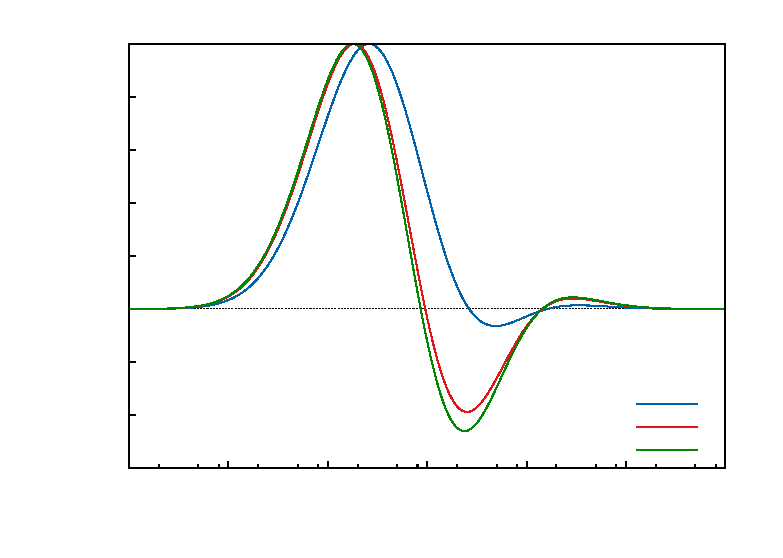
\includegraphics{./figures/elkc_th_3D_lognormal_0_constant_area}}%
    \gplfronttext
  \end{picture}%
\endgroup
}}\hspace*{\fill}
  \caption{.}
\end{figure}

                                                                                             
\bibliographystyle{ieeetr} % number, appearance order                                       
%\bibliographystyle{abbrv} % number, alphabetical order                                      
%\bibliographystyle{apalike} % full name, alphabetical order                     
%\bibliographystyle{alpha} % 3 letter name, alphabetical order                               
\bibliography{inc/biblio}                                                                          

\end{document}
